% !TEX root = 0000.tex
% Esta es la Plantilla UNAL en LaTeX
% Tesis: Resolución Cuántica de Ecuaciones Diferenciales Parciales
% Contenido tomado de main_2.tex y organizado en la Plantilla Tesis Trabajo Final UNAL 2022.
% Los cambios respecto a la plantilla original están marcados con "TESIS".
\documentclass[10pt,spanish,openany,twoside,letterpaper]{book}

%Muestra los márgenes del documento para evitar Warnings
%Para activar la siguiente línea quite el simbolo % 
%\usepackage[showframe]{geometry}

%Formato de fuentes bibliográficas
%Use el estilo bibliográfico que sea pertinente según el área de estudio APA, IEEE, etc

%Usando el paquete Natbib
% TESIS: el texto está escrito para citas numéricas (p. ej. "Evans~\cite{evans2010}"),
% por eso se usa el estilo IEEE (ieeetr) en vez del estilo autor-año dtvstyle de la plantilla.
\usepackage[numbers,sort&compress]{natbib}
%\bibpunct{[}{]}{;}{\&}{.}{}   % TESIS: configuración autor-año de la plantilla (desactivada)
%\bibliographystyle{dtvstyle}  % TESIS: estilo de la plantilla (desactivado)
\bibliographystyle{ieeetr}

%Idioma del documento
%Use main para el idioma principal del documento
\usepackage[main=spanish,english,german,french,portuguese]{babel}
% TESIS: "max", "lim" en vez de "máx", "lím" (el texto está en inglés)
\AtBeginDocument{\unaccentedoperators}

% Carácteres especiales
\usepackage{fontenc}

% Evita ligadura li & fl
\usepackage{microtype}
\DisableLigatures{encoding = *, family = *}

% Otros paquetes de tablas y colores avanzados
\usepackage{amsmath,graphicx,rotating,float,multirow}
\usepackage{longtable}
\setlength{\LTcapwidth}{6in}
\usepackage[utf8]{inputenc}
% TESIS: se reemplaza "subfigure" por "subcaption" (la tesis usa el entorno subfigure de subcaption)
\usepackage{epsfig,epic,eepic,threeparttable,amscd,here,lscape,tabularx}
\usepackage{subcaption}
\usepackage{tabu,array}
\usepackage[rgb,table]{xcolor} % TESIS: opción "table" (la usaba la tesis)

% Permite ver y configurar los parámetros de la página
\usepackage{layout}
%Hyperref permite ver las secciones del texto
\usepackage[hidelinks]{hyperref}

%Permite incluir código de cualquier lenguaje dentro del texto del documento
% TESIS: minted desactivado porque la tesis no lo usa y exige compilar con -shell-escape.
%\usepackage{minted}
\usepackage{fancyvrb}
\newenvironment{myverbatim}{\Verbatim}{\endVerbatim}

%Genera los comandos de la página de autoría
\newcommand{\studentname}{}
\newcommand{\submissiondate}{}
\newcommand{\academictitle}{}
\newcommand{\resgroupone}{}
\newcommand{\resgrouptwo}{}
\newcommand{\researchtopic}{}
\newcommand{\thesisname}{}
\newcommand{\thesisnameeng}{}
\newcommand{\thesisnamelang}{} %Usar solo si se requiere
\newcommand{\director}{}
\newcommand{\directortitle}{}
\newcommand{\codirector}{} %Usar solo si se requiere
\newcommand{\codirectortitle}{} %Usar solo si se requiere
\newcommand{\issuedate}{}
\newcommand{\palabrasclave}{}
\newcommand{\keywords}{}
\newcommand{\schlusselworter}{}
\newcommand{\palavraschave}{}
\newcommand{\sede}{}
\newcommand{\department}{}
\newcommand{\departmenttwo}{} %Usar solo si se requiere
\newcommand{\faculty}{}
\newcommand{\university}{Universidad Nacional de Colombia}

%Información de la tesis
%Diligenciar aquí los datos para su carga automática donde se requiera en el documento
%En el caso de tesis o trabajos finales, verificar que el título coincida con el aprobado por la Facultad
\renewcommand{\studentname}{Julián Sierra Salamanca}
\renewcommand{\thesisname}{Resolución Cuántica de Ecuaciones Diferenciales Parciales}
\renewcommand{\thesisnameeng}{Quantum Resolution of Partial Differential Equations}
%\renewcommand{\thesisnamelang}{Nombre del trabajo o tesis en un tercer idioma} %Usar solo si se requiere
\renewcommand{\issuedate}{2026}
\renewcommand{\submissiondate}{2026}
\renewcommand{\director}{PhD. [Nombre del Director]}
\renewcommand{\directortitle}{[Indicar si es Profesor Titular/Asociado]}
%\renewcommand{\codirector}{Prof. Dr. Co director}
%\renewcommand{\codirectortitle}{Indicar si es Profesor Titular/Asociado}
\renewcommand{\academictitle}{Magíster en Matemática Aplicada}
%\renewcommand{\resgroupone}{Grupo A (Sigla Grupo Investigación 01) }
%\renewcommand{\resgrouptwo}{Grupo B (Sigla Grupo Investigación 02) }
\renewcommand{\researchtopic}{Modelamiento Matemático y Computación Científica}
\renewcommand{\sede}{Bogotá} 
\renewcommand{\department}{Departamento de Matemáticas}
\renewcommand{\departmenttwo}{Departamento de Matemáticas}
\renewcommand{\faculty}{Facultad de Ciencias}

%Palabras clave del documento - Tener presente los Theasurus https://www.thesaurus.com/
%Disponible en 3 idiomas aunque se puede extender a francés o otro idioma
\renewcommand{\palabrasclave}{} % (mínimo 3 y máximo 7)
\renewcommand{\keywords}{}      % (3 to 7)
%\renewcommand{\schlusselworter}{}
%\renewcommand{\palavraschave}{}

% Estilo de los encabezados y pies de página
\usepackage{fancyhdr}
\fancyhf{}%
\pagestyle{fancyplain}
\textheight22.5cm \topmargin0cm \textwidth16.5cm \headheight22pt
\oddsidemargin0.5cm \evensidemargin-0.5cm%
\fancypagestyle{plain}{
\fancyhead[RO,LE]{}
\fancyhead[RE,LO]{\small \textbf{\thesisname}}
\fancyfoot[CO,CE]{\thepage}
}
\pagestyle{fancy}
\fancyhf{}%
\renewcommand{\chaptermark}[1]{\markboth{\thechapter.\; #1}{}}
\renewcommand{\sectionmark}[1]{\markright{\thesection.\; #1}{}}
\fancyhead[LO,RE]{\leftmark}
\fancyhead[RO,LE]{\rightmark}
\fancyfoot[CO,CE]{\thepage}
\thispagestyle{fancy}%

\usepackage{titlesec}
% Permite personalizar los títulos de sección y de capítulos
% hang lo deja en el mismo renglón, display lo despliega
% Elimina el "Capitulo" y deja solo el número
\titleformat{\chapter}[hang]
  {\sffamily\Huge\bfseries}{\thechapter}{0.5cm}{\sffamily\Huge}
\titleformat{\section}[hang]{\sffamily\LARGE}{\thesection}{0.5cm}{}
\titleformat{\subsection}[hang]{\sffamily\Large}{\thesubsection}{0.5cm}{}
\titleformat{\subsubsection}[hang]{\sffamily\large}{\thesubsubsection}{0.5cm}{}
\titleformat{\paragraph}[runin]{\sffamily\normalsize}{}{}{\emph}

%Coloca anexo o apéndice en la Tabla de contenido
\usepackage[toc,page]{appendix}

% Configuración de las páginas en twoside-mode
% Permite ver y configurar los parámetros de la página
\setlength{\voffset}{-0.25in}
\setlength{\headwidth}{467pt}
\setlength{\headheight}{22pt}
\setlength{\oddsidemargin}{0pt}
\setlength{\evensidemargin}{0pt}
\setlength{\marginparwidth}{0pt}
\setlength{\marginparsep}{0pt}
\setlength{\parskip}{2em}
\setlength{\footskip}{20pt}
\setlength{\textheight}{650pt}
\setlength{\textwidth}{467pt}
\setlength{\headsep}{5pt}
\setlength{\parindent}{0pt}
\setlength{\baselineskip}{10pt plus 5pt minus 5pt}
\renewcommand{\theequation}{\thechapter-\arabic{equation}}
\renewcommand{\thefigure}{\textbf{\thechapter-\arabic{figure}}}
\renewcommand{\thetable}{\textbf{\thechapter-\arabic{table}}}

%Ajusta el espacio entre la etiqueta de figuras y tablas y su título en la lista de figuras y en la de tablas 
\usepackage{titletoc} 
\titlecontents{figure}[0em]{}{\thecontentslabel\hspace{1em}}{}{\titlerule*[1pc]{.}\contentspage}
\titlecontents{table}[0em]{}{\thecontentslabel\hspace{1em}}{}{\titlerule*[1pc]{.}\contentspage}

%Define la distancia de la primera linea de un parrafo a la margen
\parindent0cm 

%Espacio entre lineas
\renewcommand{\baselinestretch}{1}

%Permite personalizar el ajuste vertical mediante cajas
\usepackage{adjustbox}

%Para rotar texto, objetos, tablas y páginas.
\usepackage{rotating}

%Permite incluir mecanismos y reacciones químicas
\usepackage{tikz}
\usepackage{chemformula}
\usepackage{chemfig}

\usetikzlibrary{calc,arrows.meta}% per right to e left to
\tikzset{
myedge/.style={->, -{Latex[#1]}}
}

%Fuente de la presentación Ancizar Sans UNAL
%Para usar este compilado en Overleaf se debe usar el compilador XeLaTeX o LuaLaTeX!!
%Menu -> Compiler -> XeLaTeX o LuaLaTeX
%La siguiente línea debe comentarse si desea compilar con pdfLaTeX
%\RequireXeTeX

% Definición de la fuente Ancizar Sans
\newif\ifxetexorluatex

\ifxetexorluatex
  \usepackage{fontspec}
  \usefonttheme{serif}
  \setmainfont{AncizarSans}[Path=./AncizarSans/,Scale=1,Extension=.otf,UprightFont=*-Regular,BoldFont=*-Bold,ItalicFont=*-Italic,BoldItalicFont=*-BoldItalic]
\else
  % Si se compila con pdfLaTeX, cargar la fuente apropiada aquí
  \usepackage[T1]{fontenc}
\fi
% Metadatos del documento
\AtBeginDocument{%
	\hypersetup{
		pdfborder={0 0 0},
		pdfauthor={\studentname},
		pdfsubject={\thesisname}, 
		pdfcreator={\studentname},
		pdfproducer={\studentname},
	}
}

%Carga el simbolo de grado y el de Angstrom
\newcommand{\angstrom}{\textup{\AA}}
\newcommand{\grad}{$^{\circ}$}

% ==========================================
% TESIS: paquetes, entornos y macros de la tesis (tomados de main_2.tex)
% ==========================================
\usepackage{amsfonts,amssymb}
\usepackage{esint}
\usepackage{amsthm}
\usepackage{booktabs}
\usepackage{mathtools}
\usepackage{mdframed}
\usepackage{bm}
\usepackage{mathrsfs}
\usepackage{algorithm}
\usepackage{algpseudocode}
\usepackage{tcolorbox}
\tcbuselibrary{breakable}

% Ubicación de las figuras (como en la plantilla, en la carpeta 00Figuras)
\graphicspath{{00Figuras/}}
\setlength{\emergencystretch}{2em} % evita líneas que se salen del margen
% Páginas que solo tienen figuras: las figuras arriba, no centradas en la página
\makeatletter
\setlength{\@fptop}{0pt}
\setlength{\@fpsep}{12pt plus 2fil}
\setlength{\@fpbot}{0pt plus 1fil}
\makeatother

% Entornos de definición, teorema, supuesto y observación
\newtcolorbox[auto counter, number within=section]{definicion}[2][]{
  colback=black!5!white, colframe=black!65!white, fonttitle=\bfseries,
  title={Definición \thetcbcounter: #2}, boxrule=0.5pt, arc=2pt, breakable, #1
}
\newtcolorbox[auto counter, number within=section]{teorema}[2][]{
  colback=black!5!white, colframe=black!80!white, fonttitle=\bfseries,
  title={Teorema \thetcbcounter: #2}, boxrule=0.5pt, arc=2pt, breakable, #1
}
\newtcolorbox[auto counter, number within=section]{supuesto}[2][]{
  colback=black!5!white, colframe=black!50!white, fonttitle=\bfseries,
  title={Supuesto \thetcbcounter: #2}, boxrule=0.5pt, arc=2pt, breakable, #1
}
\newtcolorbox{remarkbox}[1][]{
  colback=black!2!white, colframe=black!35!white, fonttitle=\bfseries,
  title={#1}, boxrule=0.5pt, arc=2pt, breakable
}

% Macros
\newcommand{\inspace}{\hspace{2ex} \text{in} \hspace{2ex}}
\newcommand{\onspace}{\hspace{2ex} \text{on} \hspace{2ex}}
\newcommand{\uxt}{u(\mathbf{x},t)}
\newcommand{\tupla}{(\mathbf{x},t)}
\newcommand{\tripla}{(\mathbf{x},t,z)}
\newcommand{\tuplapar}{(\mathbf{x}+s\mathbf{b},t+s)}
\newcommand{\ux}{u(\mathbf{x})}
\newcommand{\interception}{\cap}
\newcommand{\xy}{(\mathbf{x},\mathbf{y})}
\newcommand{\x}{(\mathbf{x})}
\newcommand{\laplacian}{\Delta}
\newcommand{\norm}[1]{\left\lVert #1 \right\rVert}
\newcommand{\abs}[1]{\left\lvert #1 \right\rvert}
\newcommand{\Loss}{\mathcal{L}}
\newcommand{\T}{\mathcal{T}}
\DeclareMathOperator*{\argmin}{arg\,min}
\DeclareMathOperator{\diag}{diag}

% Fuente de una figura o tabla (va debajo de ella): \fuente{Adaptado de Autor~\cite{...}.}
\newcommand{\fuente}[1]{\par\vspace{2pt}{\raggedright\small Fuente: #1\par}}

% Capítulos sin número (p. ej. Introducción), con el formato de la plantilla
\newcommand{\capitulosinnumero}[1]{\chapter*{\sffamily #1}\phantomsection\addcontentsline{toc}{chapter}{#1}\markboth{#1}{}\markright{}}

% Etiquetas de revisión: cambia \reviewmodetrue por \reviewmodefalse para ocultarlas
\newif\ifreviewmode
\reviewmodetrue
\newcommand{\revtag}[2]{\ifreviewmode{\color{red!70!black}\textsf{\footnotesize[#1#2]}}\fi}
\newcommand{\verificar}[1]{\revtag{VERIFICAR}{: #1}}
\newcommand{\sinfuente}[1]{\revtag{SIN\_FUENTE}{: #1}}

%Inicio del documento, no olvide la etiqueta de cierre al final \end{document}
\begin{document}

%Nombres y formatos de títulos, tablas y figuras
%Use \sffamily para dejar con letra Sans Serif, sin etiqueta queda LaTeX clásico
\renewcommand{\listfigurename}{\sffamily Lista de figuras}
\renewcommand{\listtablename}{\sffamily Lista de tablas}
\renewcommand{\contentsname}{\sffamily Contenido}
\renewcommand{\chaptername}{\sffamily Capítulo}
\renewcommand{\tablename}{\scriptsize \centering \textbf{Tabla}}
\renewcommand{\figurename}{\scriptsize \centering \textbf{Figura}}
\renewcommand{\appendixname}{\sffamily Anexo}

%Cambia el nombre de la sección de referencias
\renewcommand{\bibname}{\sffamily Referencias Bibliográficas}

%Páginas de Presentación del documento - No modificar esto se hace automáticamente
{\newpage
\thispagestyle{empty}
\begin{center}
\begin{figure}
\centering

\epsfig{file=00Figuras/00f00EscudoUN2016,scale=1}%
\end{figure}
\vspace{2.5cm}
{\Huge\bfseries\renewcommand{\baselinestretch}{1.3}\selectfont \thesisname\par} % TESIS: más espacio entre las líneas del título
\vspace{2.5cm}
\textbf{\Large \studentname} \\
\vspace{5.0cm}
\faculty \\ \department \\
\sede, Colombia\\
\issuedate
\newpage 
\thispagestyle{empty}
\vspace{2.0cm}
{\Huge\bfseries\renewcommand{\baselinestretch}{1.3}\selectfont \thesisname\par} % TESIS: más espacio entre las líneas del título
\vspace{2.0cm}
\textbf{\Large \studentname} \\
\vspace{2.0cm}
\small Tesis presentada como requisito parcial para optar por el título de: \\
{\bfseries \academictitle}\\
\vspace{2.0cm}
\textbf{Director(a):} \\
\director \\
\directortitle \; - \departmenttwo \\
\faculty \\
\university \\ 
% TESIS: sin codirector. Descomentar el bloque si se requiere.
%\vspace{0.5cm}
%\textbf{Codirector(a):} \\
%\codirector \\
%\codirectortitle \; - \department \\
%\faculty \\
%\university 
\vspace{1.5cm}
\textbf{Línea de investigación:} \\ 
\researchtopic\\
% TESIS: sin grupo de investigación. Descomentar si se requiere.
%\textbf{Grupo de investigación:} \\
%\resgroupone \\
%\resgrouptwo \\
\vspace{1.5cm} 
\university \\
\faculty \\
\department \\
\issuedate
\end{center}

% Dedicatorias
% TESIS: la tesis aún no tiene dedicatoria. Descomentar y completar si se requiere.
%\newpage
%\thispagestyle{empty}
%\begin{flushright}
%\begin{minipage}{12.5cm}
%\noindent
%\\[10em]
%%Modificar la cita que se quiere agregar
%{\Large Cita 01.}
%\\[3em]
%Autor
%\\ \textit{Fuente}
%\end{minipage}
%\end{flushright} 

% Declaracíon de originalidad del texto y del contenido
% No modificar, se hace automáticamente con los comandos ya definidos
\newpage
\chapter*{\sffamily Declaración}
\par Me permito afirmar que he realizado ésta tesis de manera autónoma y con la única ayuda de los medios permitidos y no diferentes a los mencionados el presente texto. Todos los pasajes que se han tomado de manera textual o figurativa de textos publicados y no publicados, los he reconocido en el presente trabajo. Ninguna parte del presente trabajo se ha empleado en ningún otro tipo de tesis. 
\\[1em]
\sede, \submissiondate
\\[6em]
\rule{6cm}{0.5pt}\\
\studentname
}

%Páginas preámbulo, listado de figuras, tablas y tabla de contenido
{\pagestyle{plain} \pagenumbering{roman}
\setlength{\parskip}{1mm}
% TESIS: Agradecimientos y Abreviaturas aún están vacíos; quitar el % cuando se completen.
%% !TEX root = 0000.tex
\chapter*{\sffamily Agradecimientos}
\addcontentsline{toc}{chapter}{Agradecimientos}%
%% !TEX root = 0000.tex
\chapter*{\sffamily Listado de símbolos y abreviaturas}
\addcontentsline{toc}{chapter}{Listado de símbolos y abreviaturas}
% !TEX root = 0000.tex
\newpage
\thispagestyle{empty}
\chapter*{\sffamily Resumen}
\addcontentsline{toc}{chapter}{Resumen}%
\begin{center}
\textbf{\large \thesisname}
\end{center}
% (Pega aquí tu resumen: máximo 250 palabras. Objetivos, metodología, principales resultados y conclusiones.)
\par
\vspace{2cm}

\textbf{Palabras clave:} \palabrasclave

\newpage
\thispagestyle{empty}
\chapter*{\sffamily Abstract}
\addcontentsline{toc}{chapter}{Abstract}%
\begin{center}
\textbf{\large \thesisnameeng}
\end{center}
% (Write here your abstract: at most 250 words.)
\par
\vspace{2cm}

\textbf{Keywords:} \keywords

% Resumen en un tercer idioma (opcional en la plantilla). Descomentar si se requiere.
%\newpage 
%\thispagestyle{empty}
%\chapter*{\sffamily Zusammenfassung}
%\addcontentsline{toc}{chapter}{Zusammenfassung}%
%\begin{center}
%\textbf{\large \thesisnamelang}
%\end{center}
%\par Zusammenfassung Texte.
%\\[2cm]
%\textbf{Schlüsselwörter:} \schlusselworter

% Dejar esta parte así para que genere correctamente la página de la tabla de contenido
\addcontentsline{toc}{chapter}{Lista de figuras}
\listoffigures
\clearpage
\addcontentsline{toc}{chapter}{Lista de tablas}
\listoftables
\clearpage
\addcontentsline{toc}{chapter}{Contenido}
\tableofcontents
\clearpage
}

{\pagenumbering{arabic}
\setlength{\parskip}{\baselineskip}
%Incluir secciones del documento de aqui en adelante
%Use \include para incluir desde una página nueva e \input para incluir sin salto de página
% TESIS: los objetivos están en la Introducción (sección "Justificación y objetivos").
% Planteamiento del problema, Hipótesis y Objetivos como capítulos aparte son opcionales:
%% !TEX root = 0000.tex
\chapter{Planteamiento del Problema}
\clearpage
\newpage
\chapter{Hipótesis}
%% !TEX root = 0000.tex
\chapter{Objetivos}
% !TEX root = 0000.tex
% Introducción
% Contenido tomado de main_2.tex (líneas 354-429) sin cambios de texto.

% El texto está en inglés: reglas de corte de palabra del inglés
\begin{hyphenrules}{english}

\capitulosinnumero{Introducción}\label{ch:introduction}

Partial differential equations (PDEs) are among the most powerful tools in science, economics,
engineering, and applied mathematics. They appear in models such as kinetic dynamic, Fluid and gas dynamics, Granular materials flows, semiconductor, socio-economics, among others \cite{markowich2007applied}.
Through this, we can describe and explain the multiple phenomena of concern in science. By the nature
of PDEs, these equations are used to model the behavior of fluids, bodies, molecules, proteins, and
social individuals governed by physical laws and social behavior.

Differential Galois theory for linear ordinary differential equations (ODEs) shows that only those
equations whose differential Galois group is solvable admit solutions expressible in terms of
elementary functions (exponentials, integrals, and algebraic functions)
\cite{vanderput2003}. The vast majority of higher-order linear ODEs possess
non-solvable Galois groups, which implies that their solutions lack a closed-form expression in terms
of elementary functions and must instead be solved via numerical methods such as Euler, Multisteps,  Runga-Kutta and extrapolation methods \cite{hairer1993solving, iserles1996first}.

Hence, numerical methods are the only way to obtain approximate solutions in most cases. The classical
approaches are finite difference methods (FDM) \cite{strikwerda2004}, finite element methods (FEM)
\cite{zienkiewicz2013}, and finite volume methods (FVM) \cite{moukalled2016}; each of them
discretizes the domain into small pieces forming a mesh and replaces derivatives with algebraic
operators so that the computation can be carried out. On the other hand, spectral methods consist of
projecting the solution onto a finite-dimensional subspace spanned by global basis functions, such as
trigonometric or orthogonal polynomials including Legendre and Chebyshev polynomials
\cite{shen2011}.

Even so, numerical methods suffer from the curse of dimensionality, complications from complex
geometries, nonlinearity and stiffness, lack of flexibility, and limitations in data integration
\cite{schwencke2025thesis}. Computational cost grows exponentially with the dimensionality of the
domain. Mesh-based methods require special grid treatment in cases of complex, irregular, and
time-dependent domains. Highly complex PDEs with multi-scale features often require a fine grid,
which in turn leads to high computational costs.

Due to the rapid growth of available data and computing resources, machine learning techniques have
become established tools across various sciences and disciplines. These techniques have been used in
computer vision to analyze and segment cells, leading to advances in biomedical engineering
\cite{ronneberger2015}; AlphaFold resolved the protein folding problem using attention mechanisms
to understand the relationships between amino acids in protein chains \cite{jumper2021}; and
reinforcement learning has been used to control cylinders in fluid flow to minimize aerodynamic
resistance \cite{rabault2019}.

Current engineering challenges involving large amounts of data, complex geometry, and a lack of
knowledge about the internal equations governing them, together with the boom in machine learning and
deep learning \cite{bishop2006,goodfellow2016,bach2024}, have opened the field to the development
of tools that can understand behavior alongside data and model it. Three areas have emerged from this:
data-driven learning \cite{fiorini2025,brunton2016,chen2018}, operator learning
\cite{kovachki2021,li2021fno}, and physics-informed machine learning (PIML)
\cite{raissi2019,cuomo2022}.

Many scientific problems require vast amounts of data that are often unavailable. Consequently, a
purely data-driven approach is not always the most effective way to address these challenges
\cite{wu2020}. Neural operators and physics-informed machine learning do not rely solely on
training data; instead, they leverage physical information, such as partial differential equations
(PDEs) and the necessary boundary conditions. However, these paradigms are not mutually exclusive. In
fact, hybrid approaches have demonstrated their full potential by combining assumptions about the
underlying phenomena, available data, and neural network architectures
\cite{raissi2020hidden,kissas2020,nguyen2022}.

Furthermore, these new approaches have certain limitations associated with optimization \cite{wang2021gradient,wang2022ntk,krishnapriyan2021,deshpande2022,nguyen2023} and architecture \cite{rahaman2019,cao2020spectral,wang2021deeponet}. There is gradient imbalance caused by the stiffness of the cost function, spectral bias that hinders the representation of sharp peaks, discontinuities, and propagating wave fronts, and causality issues for propagative PDEs. On the other
hand, some authors have developed theories concerning convergence
\cite{mishra2025,siegel2024,shin2020convergence}, numerical stability
\cite{deryck2024acta,dong2024}, and approximation error \cite{zeinhofer2024,chantada2024}.
For spectrum analysis and the training process, the Neural Tangent Kernel (NTK) is a powerful tool to
explain the ill-conditioning of classical PINNs \cite{jacot2018,wang2022ntk} regarding spectral
bias, stiffness, and rigid gradients.

\section*{Justificación y objetivos}\label{sec:objectives}
% TODO (required): research question, general objective and specific objectives.
% Chapters 2--4 are written so that each section can be traced to one specific objective.
% Suggested structure (adapt to your proposal):
%  OE1. Characterize the regularity of elliptic, parabolic and hyperbolic linear PDEs and its
%       consequences for physics-informed learning (Chapter 2).
%  OE2. Formalize the PINN optimization problem and the architectures used to mitigate its
%       pathologies, and propose MABUR-PINN (Chapter 3).
%  OE3. Evaluate MABUR-PINN on the linear Klein--Gordon equation and on a subset of the PINNacle
%       benchmark (Chapter 4).
%  OE4. Explore a variational quantum formulation of the problem (Chapter 5).
\verificar{NO OLVIDAR COPIAR!}

\end{hyphenrules}
 % Introducción
% !TEX root = 0000.tex
% Capítulo 1: About Partial Differential Equations
% Contenido tomado de main_2.tex (líneas 434-1565) sin cambios de texto.

% El texto está en inglés: reglas de corte de palabra del inglés
\begin{hyphenrules}{english}

\chapter{About Partial Differential Equations}\label{ch:pdes}

It is now well established that partial differential equations (PDEs) are the primary tool for
modeling phenomena in physics and engineering, and that there is no general method for solving them,
since each case has its own particularities. Modern theory divides them into two broad categories:
evolution equations and stationary equations. Traditional hyperbolic and parabolic equations are
classified as evolution equations, whereas elliptic equations are classified as stationary equations.
Consequently, numerical analysis treats the solution process separately for each case.

This chapter reviews the theoretical aspects that are fundamental when working with PDEs. In particular, as previously mentioned, each case presents its own characteristics; one of these, which we analyze throughout the chapter, is regularity. The degree of smoothness that the solution acquires, retains, or loses in relation to the initial data and source functoin. This question is not only theoretical. A physics-informed neural
network (Chapter~\ref{ch:pinns}) is a smooth function that is trained by evaluating derivatives of the
solution, so the regularity of the theorical solution decides how difficult the problem
is for the network. For that reason, every equation of Section~\ref{sec:linear-pdes} ends with a short
paragraph about its regularization, Section~\ref{sec:modern-theory} introduces the spaces where non-smooth
solutions live, Section~\ref{sec:second-order} classifies the three families that appear in our benchmark
(elliptic, parabolic and hyperbolic), and Sections~\ref{sec:regularity-bridge} and \ref{sec:klein-gordon} explain why we
chose the Klein--Gordon equation as the case study of this thesis.

The conceptual framework of this chapter is based fundamentally on the theory of partial differential
equations developed by Evans~\cite{evans2010}. Unless otherwise stated, the definitions, notations, and
theorems presented in this chapter follow the exposition of that work.

% =====================================================================
\section{Linear Partial Differential Equations}\label{sec:linear-pdes}
% =====================================================================

The four equations of this section are the prototypes of the theory: the transport equation (first
order, hyperbolic), Laplace's equation (elliptic), the heat equation (parabolic) and the wave equation
(hyperbolic). For each of them we look at the same three things: the homogeneous problem, the
non-homogeneous problem through Duhamel's principle, and the regularity of the solution.
The complete derivations of the formulas of this section, with all the intermediate steps, are in
Appendix~\ref{app:classical}. Here we present the statement of each problem, its solution, and, above all, what the solution indicates about regularity.

% ---------------------------------------------------------------------
\subsection{Transport Equation}\label{subsec:transport}

The transport equation is a natural starting point for the study of first-order partial differential
equations: it is simple enough to solve explicitly, yet it already exhibits the main features of the
theory \cite{evans2010}. It models the propagation of a physical quantity in space. Here, we only
consider a constant velocity $\mathbf{b}\in\mathbb{R}^n$ for its introduction.

The pure homogeneous or non-homogeneous transport problem is represented by a first-order differential
operator $L$, which is hyperbolic and describes the propagation or advection of a profile along
characteristic curves. Its solution, whether classical or weak, is given by a rigid translation of the
initial data, $u(\mathbf{x},t)=g(\mathbf{x}-t\mathbf{b})$.

\subsubsection{Homogeneous case}
Let $u\in C^1(\mathbb{R}^n\times[0,\infty))$ and consider the initial condition for the homogeneous problem:
\begin{equation}
  \begin{cases}
    \partial_t u(\mathbf{x},t)+\mathbf{b}\cdot\nabla u(\mathbf{x},t)=0 & \text{in } \mathbf{x}\in\mathbb{R}^n,\ t\in(0,\infty),\\
    u(\mathbf{x},0)=g(\mathbf{x}) & \text{on } \mathbf{x}\in\mathbb{R}^n,\ \{t=0\}.
  \end{cases}
  \label{eq:transport-hom}
\end{equation}
Writing the equation in matrix form with the constant space--time vector field
$\mathbf{V}=(\mathbf{b},1)^{T}\in\mathbb{R}^{n+1}$ (Appendix~\ref{app-sec:transport}), it reads
$D_{\mathbf{V}}u=\nabla_{\mathbf{x},t}u\cdot\mathbf{V}=0$, which establishes that the directional derivative of $u$ in the direction of the vector $\mathbf{V}$ is
identically zero throughout the space--time domain. This means that the velocity vector is perpendicular
to the gradient and tangent to $u$. In other words, if one moves in the direction of
$\mathbf{V}$, the value of $u$ remains constant along the characteristic trajectory. The solution to
$D_{\mathbf{V}}u=0$ is $u(\mathbf{x},t)=g(\mathbf{x}-t\mathbf{b})$.

\subsubsection{Non-homogeneous case}
To analyze the non-homogeneous case:
\begin{equation}
  \begin{cases}
    \partial_t u(\mathbf{x},t)+\mathbf{b}\cdot\nabla u(\mathbf{x},t)=f(\mathbf{x},t) & \text{in } \mathbf{x}\in\mathbb{R}^n,\ t\in(0,\infty),\\
    u(\mathbf{x},0)=g(\mathbf{x}) & \text{on } \mathbf{x}\in\mathbb{R}^n,\ \{t=0\},
  \end{cases}
  \label{eq:transport-nonhom}
\end{equation}
we can apply the same approach as in the homogeneous case: following the characteristic curve
$z(s)=u(\mathbf{x}+s\mathbf{b},t+s)$, $s\in[-t,0]$, whose derivative is $\,d z/\,d s=f(\mathbf{x}+s\mathbf{b},t+s)$,
and integrating from $-t$ to $0$ (Appendix~\ref{app-sec:transport}), we obtain the expression
\begin{equation}
  u(\mathbf{x},t)=g(\mathbf{x}-t\mathbf{b})+\int_{0}^{t}f\big(\mathbf{x}+(\tau-t)\mathbf{b},\tau\big)\,d\tau.
  \label{eq:transport-duhamel}
\end{equation}
Through Duhamel's principle, this result means that the solution is the sum of the transported initial
value $g(\mathbf{x}-t\mathbf{b})$ and the values accumulated from the source $f$, generated in the past times $\tau$
along the same characteristic curve.

\subsubsection{Regularization of transport operators}
The transport operator $L=\partial_t+\mathbf{b}\cdot\nabla$ has no regularizing effect in the interior of the
domain. This means that it conserves any roughness, sharp edge, or discontinuity of the initial
condition $g$ along the characteristic curves. To handle this problem, one can regularize the data
through mollification, or the operator through the vanishing viscosity method, which allows working
smoothly in the Sobolev spaces $W^{k,p}$ or the Lebesgue spaces $L^p$ (Section~\ref{sec:modern-theory}). We
will explore mollification here; for the vanishing viscosity method, which adds a small diffusion
$\varepsilon\Delta u$ and therefore turns the transport equation into a parabolic one, the reader is
referred to Evans~\cite{evans2010}. Given $g\in L^p(\mathbb{R}^n)$ and a standard mollifier
$\eta_\epsilon\in C_c^\infty(\mathbb{R}^n)$, we define the mollified initial condition
$g^\epsilon\in C^\infty(\mathbb{R}^n)\cap L^p(\mathbb{R}^n)$ through the convolution
\begin{equation}
  g^{\epsilon}(\mathbf{x})=(\eta_\epsilon*g)(\mathbf{x})=\int_{\mathbb{R}^n}\eta_\epsilon(\mathbf{x}-\mathbf{y})\,g(\mathbf{y})\,d\mathbf{y},
  \label{eq:mollifier}
\end{equation}
and the corresponding regularized solution
\begin{equation}
  u^{\epsilon}(\mathbf{x},t)=g^{\epsilon}(\mathbf{x}-t\mathbf{b})=(\eta_\epsilon*g)(\mathbf{x}-t\mathbf{b}).
  \label{eq:transport-mollified}
\end{equation}
As $\epsilon\to0$, the mollified $g^\epsilon$ converges to $g$ in $L^p(\mathbb{R}^n)$ for $1\le p<\infty$. That
is, mollification solves the regularization problem through the smoothing function $\eta$, and $u$ is also in $L^p$. The
smoothness depends only on the regularity of the initial data $g$; the operator itself does not add any.
% ---------------------------------------------------------------------
\subsection{Laplace's Equation}\label{subsec:laplace}

To introduce Laplace's equation, we define the Laplacian operator $\Delta u:=\nabla^2u$. Laplace's
equation is used to model equilibrium in the stationary state. Let
the flux be $\mathbf{F}(\mathbf{x},t)=-b\nabla u(\mathbf{x},t)$ with $b>0$, and let $u(\mathbf{x},t)$ represent a physical scalar
variable such as temperature, an electrostatic potential, or a mass density. In stationary equilibrium,
there is no temporal change of $u$; thus, the term $\partial_t u(\mathbf{x},t)$ is zero. For convenience, we
write $u(\mathbf{x},t)=u(\mathbf{x})$ for any value of $t>0$.
The conservation of mass requires that the flux divergence be zero, $\operatorname{div}(\mathbf{F})=0$;
consequently, the divergence of $\mathbf{F}$ is expressed as $-b\Delta u=0$. By the divergence theorem, the
integral of the Laplacian can be expressed in terms of the flux through the boundary $\partial U$ of any
subregion $U$:
\begin{equation}
  \int_U\Delta u\,d\mathbf{x}=\int_{\partial U}\nabla u\cdot\mathbf{n}\,d S,
  \label{eq:laplace-flux}
\end{equation}
which gives meaning to the Laplacian operator $\Delta$ as a measure of local disequilibrium, based on the properties of the Laplace operator. On the other hand, this means that the function $u$ in the interior of the domain neither adds nor removes flux;
that is, as we will see later, $u$ is the average of its surrounding points.

\subsubsection{Homogeneous case}
In searching for a solution to $\Delta u(\mathbf{x})=0$ for $\mathbf{x}\in\mathbb{R}^n$, Evans~\cite{evans2010} describes the
\emph{fundamental solution of Laplace's equation}, defined by
\begin{equation}
  \Phi(\mathbf{x})=
  \begin{cases}
    -\dfrac{1}{2\pi}\log\norm{\mathbf{x}}_2 & (n=2),\\[2mm]
    \dfrac{1}{n(n-2)\alpha(n)}\dfrac{1}{\norm{\mathbf{x}}_2^{\,n-2}} & (n\ge3),
  \end{cases}
  \label{eq:laplace-fundamental}
\end{equation}
where $\alpha(n)$ is the volume of the unit ball in $\mathbb{R}^n$ (for $n=1$ the analogous function is
$-\tfrac12\abs{x}$). Some important aspects to analyze are:
\begin{enumerate}
  \item The function $\Phi$ has a singular point at $\mathbf{0}$ for $n\ge2$.
  \item $\Delta\Phi=0$ for $\mathbf{x}\in\mathbb{R}^n\setminus\{\mathbf{0}\}$, but not at the point $\mathbf{0}$.
    Conceptually, $\Phi$ represents the fundamental building block; thus, at the singular point the
    fundamental solution must be understood as a distribution that contains the information of the
    point, and with the sign convention of Evans~\cite{evans2010} it satisfies $-\Delta\Phi=\delta_{\mathbf{0}}$.
  \item Equation~\eqref{eq:laplace-fundamental} does not contain boundary information, which is essential for
    engineering and science applications.
\end{enumerate}

Consequently, it is necessary to introduce more information from the problem itself through a
Dirichlet boundary condition, which specifies the values of the function on the boundary through an
arbitrary function $g(\mathbf{x})$. Thus, consider the following boundary value problem for
$\Omega\subset\mathbb{R}^n$ bounded and $u\in C^2(\bar\Omega)$:
\begin{equation}
  \begin{cases}
    \Delta u(\mathbf{x})=0 & \text{in } \mathbf{x}\in\Omega,\\
    u(\mathbf{x})=g(\mathbf{x}) & \text{on } \mathbf{x}\in\partial\Omega.
  \end{cases}
  \label{eq:laplace-dirichlet}
\end{equation}

The main idea is to find the solution $u$ using $\Phi$. In stationary problems, the value of $u$ is the
result of relaxing the system; in this case no source of perturbation exists, and the only information
that acts as a perturbation source is the boundary data $g$. Thus, the solution may be expressed as an
integral of $g$ over the boundary. Following Evans~\cite{evans2010}, Green's second identity applied to
$u$ and $\Phi$ gives a representation of $u$ that still contains the unknown normal derivative
$\partial u/\partial\mathbf{n}$ on the boundary. To eliminate it, it is necessary to build an auxiliary
(corrector) function $\phi^{\mathbf{x}}$ that is harmonic in $\Omega$ and matches the fundamental solution on
the boundary (the complete derivation is in Appendix~\ref{app-sec:laplace}). The unknown normal derivative
cancels and we finally find the solution $u$ through Green's function
$G(\mathbf{x},\mathbf{y})=\Phi(\mathbf{y}-\mathbf{x})-\phi^{\mathbf{x}}(\mathbf{y})$:
\begin{equation}
  u(\mathbf{x})=-\int_{\partial\Omega}g(\mathbf{y})\frac{\partial G}{\partial\mathbf{n}}(\mathbf{x},\mathbf{y})\,d S(\mathbf{y}),
  \label{eq:laplace-green}
\end{equation}
where $\partial G/\partial\mathbf{n}=\nabla_{\mathbf{y}}G\cdot\mathbf{n}$. Finally, we have an analytical solution through an
auxiliary function that imposes the cancellation on the boundary:
\begin{equation}
  \begin{cases}
    -\Delta_{\mathbf{y}}G(\mathbf{x},\mathbf{y})=\delta(\mathbf{x}-\mathbf{y}) & \text{in } \mathbf{y}\in\Omega,\\
    G(\mathbf{x},\mathbf{y})=0 & \text{on } \mathbf{y}\in\partial\Omega.
  \end{cases}
  \label{eq:green-function}
\end{equation}

\subsubsection{Non-homogeneous case}
The non-homogeneous case is the \emph{Poisson equation}. Consider the bounded domain $\Omega$; the
problem is given by
\begin{equation}
  \begin{cases}
    -\Delta u(\mathbf{x})=f(\mathbf{x}) & \text{in } \mathbf{x}\in\Omega,\\
    u(\mathbf{x})=h(\mathbf{x}) & \text{on } \mathbf{x}\in\partial\Omega.
  \end{cases}
  \label{eq:poisson}
\end{equation}
The source term $f$ acts as a local curvature generator and induces the perturbation of a local point
$\mathbf{x}$. With respect to the homogeneous problem, the source is added as a new term to the previous
equation by the same Green method:
\begin{equation}
  u(\mathbf{x})=\int_\Omega G(\mathbf{x},\mathbf{y})f(\mathbf{y})\,d\mathbf{y}-\int_{\partial\Omega}h(\mathbf{y})\frac{\partial G}{\partial\mathbf{n}}(\mathbf{x},\mathbf{y})\,d S(\mathbf{y}).
  \label{eq:poisson-green}
\end{equation}

\subsubsection{Regularity and some properties}
The Green's function and the Laplacian operator smooth the function through the mean-value property.
Applying Equation~\eqref{eq:laplace-green} to a ball $B(\mathbf{x},r)\subset\Omega$ centered at a point $\mathbf{x}$
inside the domain, where the normal derivative of $G$ is constant on the sphere $\partial B(\mathbf{x},r)$ and
its denominator is the surface area $\abs{\partial B(\mathbf{x},r)}=n\alpha(n)r^{n-1}$
(Appendix~\ref{app-sec:laplace}), we obtain
\begin{equation}
  u(\mathbf{x})=\frac{1}{\abs{\partial B(\mathbf{x},r)}}\int_{\partial B(\mathbf{x},r)}u(\mathbf{y})\,d S(\mathbf{y})
  =\fint_{\partial B(\mathbf{x},r)}u\,d S \qquad\text{(mean-value property)}.
  \label{eq:mvp}
\end{equation}
This argument is a heuristic version of the proof; the rigorous proof differentiates the spherical
average with respect to $r$ \cite[Section 2.2.2]{evans2010}. The mean-value property is
responsible for the smoothness of $u$ in $\Omega$, because the value of $u$ at any point $\mathbf{x}$ is
averaged over its neighborhood. The smoothness theorem for Laplace's equation states that if
$u\in C(\bar\Omega)$ satisfies the mean-value property for each ball $B(\mathbf{x},r)\subset\Omega$, then
$u\in C^\infty(\Omega)$. Furthermore, its derivatives are controlled by the derivative estimates in
Evans~\cite{evans2010}: with $k=\abs{\alpha}$, if $u$ is harmonic in $\Omega$ then
\begin{equation}
  \abs{D^\alpha u(\mathbf{x})}\le\frac{C_k}{r^{n+k}}\norm{u}_{L^1(B(\mathbf{x},r))},
  \label{eq:harmonic-estimate}
\end{equation}
which means that the $\alpha$-order derivatives of $u$ are bounded by the $L^1$ norm on the ball
$B(\mathbf{x},r)$ and the constant $C_k$. An aspect of interest to analyze is the factor $r^{-n-k}$: if $\alpha$
is of high order, the bound grows as a power of $1/r$, so the scale $r$ acts as a penalization term.
In other words, harmonic functions are infinitely smooth, but measuring finer and finer variations on a
fixed scale requires larger and larger constants.

% ---------------------------------------------------------------------
\subsection{Heat Equation}\label{subsec:heat}

Consider an open domain $\Omega\subset\mathbb{R}^n$ that contains a continuous conductor. Let $\mathbf{F}$ be the flux
vector of the scalar function $u(\mathbf{x},t)$, which changes for $t>0$. The conservation of energy yields
$u_t+\operatorname{div}\mathbf{F}=0$. If $\mathbf{F}$ is defined as $-b\nabla u$ with $b>0$, the equation is transformed
to $u_t-b\Delta u=0$, obtaining the homogeneous heat equation (in what follows $b=1$).

The temporal derivative is of first order while the spatial derivative is of second order. Looking for
solutions of the form $u(\mathbf{x},t)=t^{-\alpha}v(\mathbf{x}/t^{\beta})$, invariant under the scaling
$(\mathbf{x},t)\mapsto(\lambda^{\beta}\mathbf{x},\lambda t)$, that also conserve the thermal mass
(Appendix~\ref{app-sec:heat}), Evans~\cite{evans2010} shows that $\beta=1/2$ and $\alpha=n/2$. Thus, we obtain
\emph{the fundamental solution of the heat equation}, defined as
\begin{equation}
  \Phi(\mathbf{x},t)=
  \begin{cases}
    \dfrac{1}{(4\pi t)^{n/2}}\,e^{-\frac{\norm{\mathbf{x}}_2^2}{4t}} & (\mathbf{x}\in\mathbb{R}^n,\ t>0),\\[2mm]
    0 & (\mathbf{x}\in\mathbb{R}^n,\ t<0).
  \end{cases}
  \label{eq:heat-fundamental}
\end{equation}
In this manner, this function works similarly to the Laplace fundamental solution; that is, it also has
a singular point at $(\mathbf{0},0)$, and $\Phi(\cdot,t)\to\delta_{\mathbf{0}}$ in the sense of
distributions as $t\to0^+$.

\subsubsection{Homogeneous case}
As we saw in Laplace's equation, additional information (here, an initial condition) is necessary to
find a unique solution which is not trivial. Let $u\in C^{2,1}(\mathbb{R}^n\times(0,\infty))$ and consider the
Cauchy problem
\begin{equation}
  \begin{cases}
    \partial_t u(\mathbf{x},t)-\Delta u(\mathbf{x},t)=0 & \text{in } \mathbf{x}\in\mathbb{R}^n,\ t\in(0,\infty),\\
    u(\mathbf{x},0)=h(\mathbf{x}) & \text{on } \mathbf{x}\in\mathbb{R}^n,\ \{t=0\}.
  \end{cases}
  \label{eq:heat-cauchy}
\end{equation}
As a first approach, the solution is given by the convolution of the fundamental solution $\Phi$ and
the initial condition $h$:
\begin{equation}
  u(\mathbf{x},t)=(\Phi(\cdot,t)*h)(\mathbf{x})=\frac{1}{(4\pi t)^{n/2}}\int_{\mathbb{R}^n}h(\mathbf{y})\,
  e^{-\frac{\norm{\mathbf{x}-\mathbf{y}}_2^2}{4t}}\,d\mathbf{y}\qquad(\mathbf{x}\in\mathbb{R}^n,\ t>0).
  \label{eq:heat-convolution}
\end{equation}
However, we need a closed analytical form for a bounded domain $\Omega\subset\mathbb{R}^n$:
\begin{equation}
  \begin{cases}
    \partial_t u(\mathbf{x},t)-\Delta u(\mathbf{x},t)=0 & \text{in } \mathbf{x}\in\Omega,\ t\in(0,\infty),\\
    u(\mathbf{x},0)=h(\mathbf{x}) & \text{on } \mathbf{x}\in\Omega,\ \{t=0\},\\
    u(\mathbf{x},t)=g(\mathbf{x},t) & \text{on } \mathbf{x}\in\partial\Omega,\ t\in(0,\infty),
  \end{cases}
  \label{eq:heat-ibvp}
\end{equation}
which the previous formula does not include. Again, we must appeal to a Green's function. Applying the
second Green's identity to the heat operator $L=\partial_s-\Delta$ and to its adjoint (backward) operator
$L^{*}=-\partial_s-\Delta$, and building, as in Laplace's equation, an auxiliary function
$\phi^{\mathbf{x}}(\mathbf{y},\tau)$ that solves the heat equation with boundary values
$\Phi(\mathbf{x}-\mathbf{y},\tau)$ (Appendix~\ref{app-sec:heat}), we define the Green's function
$G(\mathbf{x},\mathbf{y},\tau)=\Phi(\mathbf{x}-\mathbf{y},\tau)-\phi^{\mathbf{x}}(\mathbf{y},\tau)$, which vanishes for
$\mathbf{y}\in\partial\Omega$, and the unknown term disappears. We obtain the closed form
\begin{equation}
  u(\mathbf{x},t)=\int_\Omega h(\mathbf{y})G(\mathbf{x},\mathbf{y},t)\,d\mathbf{y}
  -\int_0^t\!\!\int_{\partial\Omega}g(\mathbf{y},s)\frac{\partial G}{\partial\mathbf{n}}(\mathbf{x},\mathbf{y},t-s)\,d S(\mathbf{y})\,d s,
  \label{eq:heat-green}
\end{equation}
where $\partial G/\partial\mathbf{n}=\nabla_{\mathbf{y}}G\cdot\mathbf{n}$. The structure is exactly the same as
Equation~\eqref{eq:laplace-green}: an integral of the data against a kernel that already knows the boundary.

\subsubsection{Non-homogeneous equation -- Duhamel's principle}
Consider the non-homogeneous problem
\begin{equation}
  \begin{cases}
    \partial_t u(\mathbf{x},t)-\Delta u(\mathbf{x},t)=f(\mathbf{x},t) & \text{in } \mathbf{x}\in\mathbb{R}^n,\ t\in(0,T],\\
    u(\mathbf{x},0)=h(\mathbf{x}) & \text{on } \mathbf{x}\in\mathbb{R}^n,\ \{t=0\}.
  \end{cases}
  \label{eq:heat-nonhom}
\end{equation}
Duhamel's principle interprets the forcing term $f(\mathbf{x},t)$ as an accumulation of initial conditions for
the homogeneous problem. The solution is constructed from
\begin{equation}
  u(\mathbf{x},t)=\int_{\mathbb{R}^n}\Phi(\mathbf{x}-\mathbf{y},t)h(\mathbf{y})\,d\mathbf{y}+\int_0^t\!\!\int_{\mathbb{R}^n}\Phi(\mathbf{x}-\mathbf{y},t-s)f(\mathbf{y},s)\,d\mathbf{y}\,d s,
  \label{eq:heat-duhamel}
\end{equation}
where, for example, $f\in C_1^2(\mathbb{R}^n\times[0,\infty))$ with compact support guarantees that this
formula is a classical solution \cite{evans2010}. In a bounded domain we encounter the same issue
as in the homogeneous case, and the Green's function is used again to finally obtain
\begin{multline}
  u(\mathbf{x},t)=\int_\Omega h(\mathbf{y})G(\mathbf{x},\mathbf{y},t)\,d\mathbf{y}
  -\int_0^t\!\!\int_{\partial\Omega}g(\mathbf{y},s)\frac{\partial G}{\partial\mathbf{n}}(\mathbf{x},\mathbf{y},t-s)\,d S(\mathbf{y})\,d s\\
  +\int_0^t\!\!\int_\Omega f(\mathbf{y},s)G(\mathbf{x},\mathbf{y},t-s)\,d\mathbf{y}\,d s.
  \label{eq:heat-green-full}
\end{multline}

\subsubsection{Regularization and some properties}
The fundamental solution of the heat equation is a Gaussian function (the heat kernel). Some of its
properties are smoothness, boundedness, and decay to $0$ as $\norm{\mathbf{x}}\to\infty$. For those reasons,
the heat kernel propagates with apparently infinite velocity: a change in the value of $u$ at a point
$\mathbf{x}$ has an immediate effect at any point $\mathbf{y}$ with $\operatorname{dist}(\mathbf{x},\mathbf{y})>0$, as if it were
moving with infinite velocity.

This kernel acts as a filter for corners, edges, and discontinuities. To see it, take a compact set $K$
inside an open set $V$ of space--time, $K\subset\subset V$, and a cutoff function
$\zeta\in C_c^\infty(\mathbb{R}^n\times(0,T))$ that equals one in $K$ and zero outside $V$. The function
$v=u\zeta$ solves the heat equation with a source that only contains $u$, $\nabla u$ and the derivatives
of $\zeta$. Writing the Duhamel solution \eqref{eq:heat-duhamel} for $v$ and moving the derivative from $u$
to the known functions (Appendix~\ref{app-sec:heat}), we arrive at
\begin{equation}
  v(\mathbf{x},t)=\int_0^t\!\!\int_{\mathbb{R}^n}u(\mathbf{y},s)\,\mathcal{K}(\mathbf{x},\mathbf{y},t,s)\,d\mathbf{y}\,d s,
  \qquad\mathcal{K}=\Phi\,(\partial_s\zeta+\Delta\zeta)+2\nabla\Phi\cdot\nabla\zeta,
  \label{eq:cut-9}
\end{equation}
where $\Phi=\Phi(\mathbf{x}-\mathbf{y},t-s)$ and all derivatives act on $\mathbf{y}$. Here is the key point: the kernel $\mathcal{K}$ only contains derivatives of $\zeta$, which vanish
near $K$. Therefore, for $(\mathbf{x},t)$ inside $K$ the kernel never touches the singularity of $\Phi$ and
$\mathcal{K}$ is $C^\infty$ in $(\mathbf{x},t)$. Since $v=u$ in $K$, Equation~\eqref{eq:cut-9} says that $u$ is
infinitely smooth there, whatever the roughness of $u$ outside. The estimation theorem in the heat
equation section of Evans~\cite{evans2010} establishes, moreover, that its derivatives are bounded on
parabolic cylinders $C(\mathbf{x},t;r)$:
\begin{equation}
  \max_{C(\mathbf{x},t;r/2)}\abs{D_{\mathbf{x}}^{k}D_t^{l}u}\le\frac{C_{kl}}{r^{k+2l+n+2}}\norm{u}_{L^1(C(\mathbf{x},t;r))}.
  \label{eq:heat-estimate}
\end{equation}
Equation~\eqref{eq:heat-estimate} offers a clear perspective on the regularization of the heat equation. The
structure here takes the form of
\[
  \begin{gathered}
  \text{Maximum change in some region}\\
  \le\ \text{Total heat of a bigger region}\times\text{Geometric constant};
  \end{gathered}
\]
the space--time derivatives of $u$ on a parabolic cylinder are bounded by the local $L^1$ norm of $u$
and a constant $C_{kl}$, meaning that the variation of $u$ at an arbitrary point of $C(\mathbf{x},t;r/2)$ is
governed by the total heat of the region where it is contained. The bound depends on the geometric factor
$r^{-(k+2l+n+2)}$; taking higher derivatives makes this factor increasingly larger, reflecting that
measuring finer variations requires a larger bound when the scale $r$ is fixed. This is how the
equation handles any irregular behavior of the data $g$ or $h$: after any positive time, it has been
filtered out.

% ---------------------------------------------------------------------
\subsection{Wave Equation}\label{subsec:wave}

The heat equation introduces a first-order time derivative alongside the Laplacian operator, giving
rise to a local property: the update of the local disequilibrium measure, that is to say, a continuous
adaptation to the surrounding points (diffusion). Increasing the order of the time derivative by one
causes a wave propagation phenomenon:
\begin{equation}
  \partial_t^2u(\mathbf{x},t)-\Delta u(\mathbf{x},t)=0\qquad\text{in } \mathbf{x}\in\mathbb{R}^n,\ t\in[0,T].
  \label{eq:wave}
\end{equation}

\subsubsection{Homogeneous case}
Let $u\in C^2(\mathbb{R}^n\times[0,\infty))$ be a function that solves the wave equation for $\mathbf{x}\in\mathbb{R}^n$ and
$t>0$. Given the initial data $g$ and $h$, the homogeneous problem is defined as
\begin{equation}
  \begin{cases}
    \partial_t^2u(\mathbf{x},t)-\Delta u(\mathbf{x},t)=0 & \text{in } \mathbf{x}\in\mathbb{R}^n,\ t\in(0,T],\\
    u(\mathbf{x},0)=g(\mathbf{x}) & \text{on } \mathbf{x}\in\mathbb{R}^n,\ \{t=0\},\\
    \partial_t u(\mathbf{x},0)=h(\mathbf{x}) & \text{on } \mathbf{x}\in\mathbb{R}^n,\ \{t=0\}.
  \end{cases}
  \label{eq:wave-cauchy}
\end{equation}
With the aim of solving this, Evans~\cite{evans2010} shows that the closed forms depend on the dimension.

\textbf{Case $n=1$: d'Alembert's formula.}
D'Alembert's formula takes advantage of the factorization of the wave operator into two transport
operators, $\Box=\partial_t^2-\partial_x^2=(\partial_t+\partial_x)(\partial_t-\partial_x)$. Solving one
homogeneous and one non-homogeneous transport problem with Equation~\eqref{eq:transport-duhamel}
(Appendix~\ref{app-sec:wave}), we obtain
\begin{equation}
  u(x,t)=\frac12\big[g(x+t)+g(x-t)\big]+\frac12\int_{x-t}^{x+t}h(y)\,d y.
  \label{eq:dalembert}
\end{equation}
This is d'Alembert's formula.

\textbf{Case $n\ge2$: spherical averages.}
For finding a solution in dimensions $n\ge2$, it is necessary to return to the concept of average
introduced in Laplace's equation, to analyze what happens with the surrounding points of a particular
point. Evans~\cite{evans2010} works with the mean value of $u$ over the sphere $\partial B(\mathbf{x},r)$,
which satisfies the Euler--Poisson--Darboux equation (Appendix~\ref{app-sec:wave}), and distinguishes the
solution between odd and even dimensions.

\textbf{Solution for odd $n$.}
Suppose $u\in C^2(\mathbb{R}^n\times[0,\infty))$ is a solution to the Cauchy problem for the wave equation for
$\mathbf{x}\in\mathbb{R}^n$ and $t>0$, where $n\ge3$ is odd. Also suppose that $g\in C^{m+1}(\mathbb{R}^n)$ and
$h\in C^m(\mathbb{R}^n)$, where $m=(n+1)/2$. The closed-form analytical expression that solves this case is
given by \cite{evans2010}
\begin{multline}
  u(\mathbf{x},t)=\frac{1}{\gamma_n}\Bigg[\partial_t\Big(\frac1t\partial_t\Big)^{\frac{n-3}{2}}
    \Big(t^{n-2}\fint_{\partial B(\mathbf{x},t)}g\,d S\Big)\\
    +\Big(\frac1t\partial_t\Big)^{\frac{n-3}{2}}\Big(t^{n-2}\fint_{\partial B(\mathbf{x},t)}h\,d S\Big)\Bigg],
  \label{eq:wave-odd}
\end{multline}
where $\gamma_n=1\cdot3\cdot5\cdots(n-2)$. It only requires knowing the functions $g$ and $h$ over the
sphere $\partial B(\mathbf{x},t)=\{\mathbf{y}\in\mathbb{R}^n\mid\norm{\mathbf{y}-\mathbf{x}}_2=t\}$, which is the base of the backward light
cone with vertex $(\mathbf{x},t)$. This represents a light front because the Minkowski space--time interval is
$s^2=(ct)^2-\norm{\mathbf{y}-\mathbf{x}}_2^2$. For a light-like path the interval of wave propagation is $s^2=0$,
assuming the wave speed is $c=1$. This means that the distance between two points of the spatial domain
is equal to the time. Geometrically, this boundary is a sphere in the spatial domain, centered at $\mathbf{x}$
with radius $t$. The fact that the solution depends only on this surface, and not on the interior of
the ball, is the mathematical statement of Huygens' principle: information propagates exactly at the
speed $c$ without leaving a residual trail. Whatever happens inside the ball does not affect $u(\mathbf{x},t)$.

\textbf{Solution for even $n$.}
Suppose $u\in C^2(\mathbb{R}^n\times[0,\infty))$ is a solution to the Cauchy problem for the wave equation for
$\mathbf{x}\in\mathbb{R}^n$ and $t>0$, where $n$ is even. Also suppose that $g\in C^{m+1}(\mathbb{R}^n)$ and $h\in C^m(\mathbb{R}^n)$,
where $m=(n+2)/2$. The closed-form analytical expression that solves this case is given by the method
of descent \cite{evans2010}:
\begin{multline}
  u(\mathbf{x},t)=\frac{1}{\gamma_n}\Bigg[\partial_t\Big(\frac1t\partial_t\Big)^{\frac{n-2}{2}}
    \Big(t^{n}\fint_{B(\mathbf{x},t)}\frac{g(\mathbf{y})}{(t^2-\norm{\mathbf{y}-\mathbf{x}}_2^2)^{1/2}}\,d\mathbf{y}\Big)\\
    +\Big(\frac1t\partial_t\Big)^{\frac{n-2}{2}}
    \Big(t^{n}\fint_{B(\mathbf{x},t)}\frac{h(\mathbf{y})}{(t^2-\norm{\mathbf{y}-\mathbf{x}}_2^2)^{1/2}}\,d\mathbf{y}\Big)\Bigg],
  \label{eq:wave-even}
\end{multline}
where $\gamma_n=2\cdot4\cdots(n-2)\cdot n$. It requires knowing the functions $g$ and $h$ over the
entire volume of the solid ball $B(\mathbf{x},t)$; here, what happens inside the solid ball does affect
$u(\mathbf{x},t)$. This is reflected in the non-zero weight given by $(t^2-\norm{\mathbf{y}-\mathbf{x}}_2^2)^{-1/2}$ inside the
ball. Thus, $s^2=(ct)^2-\norm{\mathbf{y}-\mathbf{x}}_2^2>0$, meaning that the elapsed time is greater than the spatial
distance. This implies that the wave leaves a wake and interacts with points inside the solid ball.

\subsubsection{Non-homogeneous case}
By the linearity of the wave operator $\Box=\partial_t^2-\Delta$, the solution to the non-homogeneous
Cauchy problem can be decomposed by superposition as $u=u_{\mathrm{hom}}+u_{\mathrm{part}}$, where
$u_{\mathrm{hom}}$ solves the homogeneous problem determined by the initial data $g$ and $h$, and
$u_{\mathrm{part}}$ solves the problem with source $f$ and zero initial conditions. To construct
$u_{\mathrm{part}}$, we apply Duhamel's principle. Rather than treating the source $f$ as a global
function in time, we interpret it as a continuous superposition of instantaneous impulses. For each
instant $s\in[0,t]$, consider the following auxiliary initial value problem:
\begin{equation}
  \begin{cases}
    \partial_t^2u(\mathbf{x},t;s)-\Delta u(\mathbf{x},t;s)=0 & \text{in } \mathbf{x}\in\mathbb{R}^n,\ t\in(s,\infty),\\
    u(\mathbf{x},s;s)=0 & \text{on } \mathbf{x}\in\mathbb{R}^n,\ \{t=s\},\\
    \partial_t u(\mathbf{x},s;s)=f(\mathbf{x},s) & \text{on } \mathbf{x}\in\mathbb{R}^n,\ \{t=s\}.
  \end{cases}
  \label{eq:wave-duhamel-aux}
\end{equation}
By Duhamel's principle, the solution to the non-homogeneous problem is obtained by integrating all
these auxiliary solutions over all past times $s$. The micro-source $f(\mathbf{x},s)$ can be seen as a local
property: a micro-perturbation occurring at time $s$ gives a pulse to the system that is converted into
velocity, while the position at that instant is not changed (the initial position of each auxiliary
problem is zero). The solution is expressed as
\begin{equation}
  u_{\mathrm{part}}(\mathbf{x},t)=\int_0^t u(\mathbf{x},t;s)\,d s.
  \label{eq:wave-duhamel}
\end{equation}

\subsubsection{About the problem of solutions with closed forms}
Commenting on closed forms, Evans \cite[p.~82]{evans2010} argues: ``the explicit formulas demonstrate the necessity of making more and more smoothness assumptions upon the data $g$ and $h$ to ensure the existence of a $C^2$ solution of the wave equation for larger and larger $n$''. The wave operator, unlike the Laplace
and heat operators, does not produce a smoothing estimate like the ones in
Equations~\eqref{eq:harmonic-estimate} and \eqref{eq:heat-estimate}, the regularity of $\uxt$ is exactly the regularity
of the initial data, and singularities travel along the light cone. Thus, the modern theory of PDEs is needed
to handle problems without so many assumptions about the regularity of the initial data $g$ and $h$,
and of course about $u$.

% =====================================================================
\section{Modern Theory of Partial Differential Equations}\label{sec:modern-theory}
% =====================================================================

The classical theory of PDEs faces limitations when handling real problems. As discussed in the
previous sections, the existence of classical $C^2$ solutions imposes strict regularity requirements on
the initial data and boundary data. For the wave equation, highly smooth data $g\in C^{m+1}$ and
$h\in C^m$ are required. For Laplace's equation, the domain boundaries must be smooth enough for the
Green's function to exist, and corners produce singularities. Even for the heat equation, discontinuous
initial data or sources prevent the existence of a classical solution at $t=0$. These strict
requirements fail to represent most cases that science or engineering must address, where data often
present discontinuities, geometric corners, or lack high regularity. It is necessary to formulate a more
flexible framework. To respond to that, modern PDE theory requires tools that can handle them. In this
section, we address this through Hölder spaces, Lebesgue spaces, weak derivatives, Sobolev spaces and
weak solutions.

% ---------------------------------------------------------------------
\subsection{Hölder Spaces}\label{subsec:holder}

Some functions are perfect candidates for the classical framework, but irregular functions are better
suited to represent the real world. How can one measure the derivative of a function that is not
differentiable? To address this question, the Hölder norm avoids differentiation and measures, instead,
how fast the function can oscillate \cite{evans2010}:

\begin{definicion}{Hölder norm.}\label{def:holder-norm}
Let $\Omega\subset\mathbb{R}^n$ be an open set and $u:\Omega\to\mathbb{R}$ a bounded and continuous function. The
supremum norm is defined as
\[
  \norm{u}_{C^0(\bar\Omega)}:=\sup_{\mathbf{x}\in\Omega}\abs{u(\mathbf{x})}.
\]
The Hölder seminorm of $u$ with exponent $0<\gamma\le1$ is given by
\[
  [u]_{C^{0,\gamma}(\bar\Omega)}:=\sup_{\substack{\mathbf{x},\mathbf{y}\in\Omega\\ \mathbf{x}\neq\mathbf{y}}}
  \frac{\abs{u(\mathbf{x})-u(\mathbf{y})}}{\abs{\mathbf{x}-\mathbf{y}}^{\gamma}},
\]
and the Hölder norm is then defined as
$\norm{u}_{C^{0,\gamma}(\bar\Omega)}:=\norm{u}_{C^0(\bar\Omega)}+[u]_{C^{0,\gamma}(\bar\Omega)}$.
\end{definicion}

\begin{definicion}{Hölder space.}\label{def:holder-space}
The Hölder space $C^{k,\gamma}(\bar\Omega)$ consists of all functions $u\in C^k(\bar\Omega)$ for which
the norm
\begin{equation}
  \norm{u}_{C^{k,\gamma}(\bar\Omega)}:=\sum_{\abs{\alpha}\le k}\norm{D^\alpha u}_{C^0(\bar\Omega)}
  +\sum_{\abs{\alpha}=k}[D^\alpha u]_{C^{0,\gamma}(\bar\Omega)}
  \label{eq:holder-norm}
\end{equation}
is finite.
\end{definicion}

The case $\gamma=1$ is Lipschitz continuity, so Hölder continuity is a generalization of it in which the
``slope'' is allowed to blow up in a controlled way. Evans~\cite{evans2010} establishes that every space
$C^{k,\gamma}(\bar\Omega)$ is a Banach space, that is, it is complete, which is what one needs for
convergence and fixed-point arguments. However, this is not enough. Having a function that is smooth
everywhere except at a few points relaxes the rigid regularity assumptions on the initial and boundary
data, but it does not resolve the PDE problem, because the equation still asks for classical
derivatives. A Hölder norm only gives knowledge of the local oscillations of the function and of its
supremum value. We will meet the Hölder seminorm again in Chapter~\ref{ch:pinns}, where it is used to
regularize the loss function of a PINN \cite{shin2020convergence}.

% ---------------------------------------------------------------------
\subsection{Lebesgue Spaces $L^p$}\label{subsec:lp}

To rigorously define the modern formulation, we introduce the Lebesgue spaces, following
Castillo~\cite{castillo2014}.

\begin{definicion}{$L^p$ space.}\label{def:lp}
Let $\Omega\subset\mathbb{R}^n$ be an open domain and $p\in[1,\infty)$. The space $L^p(\Omega)$ consists of all
(classes of) measurable functions whose $p$-th power is Lebesgue integrable:
\begin{equation}
  L^p(\Omega):=\Big\{f:\Omega\to\mathbb{R}\ \Big|\ \int_\Omega\abs{f(\mathbf{x})}^p\,d\mathbf{x}<\infty\Big\}.
  \label{eq:lp}
\end{equation}
\end{definicion}

In particular, the space $L^2(\Omega)$ is a Hilbert space equipped with the inner product
$\langle f,g\rangle_{L^2}=\int_\Omega fg\,d\mathbf{x}$, meaning that it contains functions with finite energy that
may present discontinuities. This is exactly the space in which the loss functions of
Chapter~\ref{ch:pinns} are measured.

% ---------------------------------------------------------------------
\subsection{Weak Derivatives}\label{subsec:weak}

Consider the Poisson equation \eqref{eq:poisson} with $h=0$. From Evans~\cite{evans2010}, the solution uses
the Green's function $G$ and integrates it against the source $f$:
\[
  u(\mathbf{x})=\int_\Omega G(\mathbf{x},\mathbf{y})f(\mathbf{y})\,d\mathbf{y}.
\]
However, this representation requires knowledge of the auxiliary function $\phi^{\mathbf{x}}$ (the corrector),
which is not an easy task because geometries are complex and finding such functions is difficult. Even
if a solution can be found, we must solve a homogeneous Dirichlet problem infinitely many times, one
for each point $\mathbf{x}$, which requires a high computational cost. Moreover, since $\Phi$ is a singular
function, the source $f$ must be regular enough (for example, Hölder continuous) for $u$ to be a
classical $C^2$ solution.\verificar{precise hypothesis on $f$, e.g.\ Gilbarg--Trudinger}

Instead of looking for $u$ through the kernel $G$, we test the equation against a smooth function
$\phi$ that is compactly supported, $\phi\in C_c^\infty(\Omega)$ \cite{reyna_sobolev}:
\begin{equation}
  \int_\Omega-\Delta u(\mathbf{y})\,\phi(\mathbf{y})\,d\mathbf{y}=\int_\Omega f(\mathbf{y})\phi(\mathbf{y})\,d\mathbf{y}.
  \label{eq:poisson-tested}
\end{equation}
For the identity $\phi\Delta u=\operatorname{div}(\phi\nabla u)-\nabla u\cdot\nabla\phi$:
\begin{align*}
  \int_\Omega\nabla u\cdot\nabla\phi\,d\mathbf{y}-\int_\Omega\operatorname{div}(\phi\nabla u)\,d\mathbf{y}
    &=\int_\Omega f\phi\,d\mathbf{y},\\
  \int_\Omega\nabla u\cdot\nabla\phi\,d\mathbf{y}-\int_{\partial\Omega}\phi\frac{\partial u}{\partial\mathbf{n}}\,d S(\mathbf{y})
    &=\int_\Omega f\phi\,d\mathbf{y}.
\end{align*}
Since $\phi=0$ on the boundary,
\begin{equation}
  \int_\Omega\nabla u\cdot\nabla\phi\,d\mathbf{y}=\int_\Omega f\phi\,d\mathbf{y}.
  \label{eq:poisson-weak1}
\end{equation}
If we now use $u\Delta\phi=\operatorname{div}(u\nabla\phi)-\nabla u\cdot\nabla\phi$ and apply it,
\[
  \int_\Omega u\Delta\phi\,d\mathbf{y}=\int_{\partial\Omega}u\frac{\partial\phi}{\partial\mathbf{n}}\,d S(\mathbf{y})
  -\int_\Omega\nabla u\cdot\nabla\phi\,d\mathbf{y}=-\int_\Omega\nabla u\cdot\nabla\phi\,d\mathbf{y},
\]
and finally it comes to
\begin{equation}
  \int_\Omega u\Delta\phi\,d\mathbf{y}=-\int_\Omega f\phi\,d\mathbf{y}.
  \label{eq:poisson-weak2}
\end{equation}
In Equation~\eqref{eq:poisson-weak2} there is no derivative of $u$ at all: all of them were transferred to the
test function. And, applying the Cauchy--Schwarz inequality \cite{castillo2014},
\begin{equation}
  \Big|\int_\Omega f\phi\,d\mathbf{y}\Big|\le\Big(\int_\Omega f^2\,d\mathbf{y}\Big)^{1/2}\Big(\int_\Omega\phi^2\,d\mathbf{y}\Big)^{1/2}
  =\norm{f}_{L^2(\Omega)}\norm{\phi}_{L^2(\Omega)},
  \label{eq:cauchy-schwarz}
\end{equation}
so the right-hand side makes sense as soon as $f\in L^2(\Omega)$. Here we observe that this weak
formulation relaxes the regularity requirements: instead of requiring a classical $C^2$ solution and a
Hölder continuous source $f$, as demanded by the classical Green's function representation, the weak
theory only requires $f\in L^2(\Omega)$ (or even $f\in H^{-1}(\Omega)$) and seeks the solution $u$ in a
Sobolev space \cite{castillo2014}. Being able to represent the solution through a source $f$
residing in a less regular space, while still guaranteeing the existence of a solution, is a major
advance of the modern theory. What we did with $\Delta$ is a particular case of the following
definition.

\begin{definicion}{Weak derivative (derivative in the sense of distributions).}\label{def:weak-derivative}
Given $u\in L^1_{\mathrm{loc}}(\Omega)$ and a multi-index $\alpha$, we say that
$v_\alpha\in L^1_{\mathrm{loc}}(\Omega)$ is the $\alpha$-th weak derivative of $u$, and we write
$D^\alpha u:=v_\alpha$, if for every test function $\phi\in C_c^\infty(\Omega)$ it holds that
\cite{reyna_sobolev}
\begin{equation}
  \int_\Omega u\,D^\alpha\phi\,d\mathbf{y}=(-1)^{\abs{\alpha}}\int_\Omega v_\alpha\,\phi\,d\mathbf{y}.
  \label{eq:weak-derivative}
\end{equation}
\end{definicion}

In our Poisson case we already have this result, but seen in another way. If we organize it a little,
with $\abs{\alpha}=2$ the sign is $(-1)^2=1$ and
\begin{equation}
  \int_\Omega u\Delta\phi\,d\mathbf{y}=(-1)^2\int_\Omega\Delta u\,\phi\,d\mathbf{y}=-\int_\Omega f\phi\,d\mathbf{y},
  \label{eq:weak-poisson-again}
\end{equation}
which is Equation~\eqref{eq:poisson-weak2}. The weak Laplacian of $u$ is $-f$, even if $u$ has no classical second
derivatives.

% ---------------------------------------------------------------------
\subsection{Sobolev Spaces}\label{subsec:sobolev}

While the Lebesgue spaces $L^p(\Omega)$ provide a framework for functions with finite energy, they do
not account for the behavior of their derivatives. To rigorously measure the regularity of a function
alongside its weak derivatives, we introduce the Sobolev spaces.

\begin{definicion}{Sobolev spaces.}\label{def:sobolev}
Let $\Omega\subset\mathbb{R}^n$ be an open domain, $k\in\mathbb{N}$ and $1\le p<\infty$. The Sobolev space
$W^{k,p}(\Omega)$ consists of all functions $u\in L^p(\Omega)$ whose weak derivatives $D^\alpha u$ up to
order $k$ also belong to $L^p(\Omega)$. That is:
\begin{equation}
  W^{k,p}(\Omega):=\big\{u\in L^p(\Omega)\ \big|\ D^\alpha u\in L^p(\Omega)\ \ \forall\,\abs{\alpha}\le k\big\}.
  \label{eq:sobolev}
\end{equation}
In the specific case $p=2$, we denote this space as $H^k(\Omega):=W^{k,2}(\Omega)$. The space
$H^1(\Omega)$ is a Hilbert space equipped with the inner product
\begin{equation}
  \langle u,v\rangle_{H^1(\Omega)}:=\int_\Omega uv\,d\mathbf{y}+\int_\Omega\nabla u\cdot\nabla v\,d\mathbf{y}.
  \label{eq:h1-inner}
\end{equation}
\end{definicion}

The space $H^1_0(\Omega)$ is defined as the closure of $C_c^\infty(\Omega)$ in $H^1(\Omega)$. It means
that every function of $H^1_0(\Omega)$ can be approximated, in the energy norm, by smooth functions with
compact support; this is how the space encodes the zero boundary condition (in the sense of traces)
without asking the function to be smooth: it may have corners or kinks, as long as its energy does not
blow up. Since the weak formulation Equation~\eqref{eq:poisson-weak1} involves the gradients $\nabla u$ and
$\nabla\phi$, $H^1_0(\Omega)$ is the natural space for the solution of the Poisson problem with zero
boundary data. On the other hand, the space $H^2(\Omega)$ consists of functions whose weak derivatives
up to second order belong to $L^2(\Omega)$; this is the natural space for operators involving the
Laplacian $\Delta u$ or second temporal derivatives $\partial_{tt}u$ in strong form, as it guarantees
that both the function and its curvature have finite energy. Finally, $H^{-1}(\Omega)$ denotes the
topological dual space of $H^1_0(\Omega)$. While $H^1_0(\Omega)$ is the space of states with finite
energy, $H^{-1}(\Omega)$ is the space of forces or sources.

This difference between $H^1$ (weak form) and $H^2$ (strong form) will be important later: a standard
PINN minimizes the \emph{strong} residual in $L^2$ (Chapter~\ref{ch:pinns}), which implicitly asks the
solution to live in $H^2$, while the weak theory only needs $H^1$.

% =====================================================================
\section{Second-Order Partial Differential Equations}\label{sec:second-order}
% =====================================================================

The four prototypes of Section~\ref{sec:linear-pdes} are particular cases of three general families. In this
section we write each family in divergence form, with variable coefficients, and we collect the
properties that Evans~\cite{evans2010} proves for their weak solutions: existence, regularity, maximum
principle and spectral representation. Throughout, $\Omega\subset\mathbb{R}^n$ is a bounded open set with
smooth boundary and $\Omega_T=\Omega\times(0,T]$.

% ---------------------------------------------------------------------
\subsection{Second-Order Elliptic Equations}\label{subsec:elliptic}

\subsubsection{The mathematical definition of ellipticity}
Let us consider the second-order linear operator in divergence form
\begin{equation}
  Lu:=-\nabla\cdot\big(A(\mathbf{x})\nabla u\big)+\mathbf{b}(\mathbf{x})\cdot\nabla u+c(\mathbf{x})u,
  \label{eq:elliptic-op}
\end{equation}
where the first term, with the symmetric matrix $A(\mathbf{x})=[a_{ij}(\mathbf{x})]$ that measures the conductivity or
tension of the medium at the point $\mathbf{x}$, is responsible for diffusion; the second term,
with $\mathbf{b}(\mathbf{x})$, is responsible for the drift of the medium; and finally, the third term, with $c(\mathbf{x})$,
acts as a local source or absorption. We say that $L$ is \emph{uniformly elliptic} if there exists a
constant $\theta>0$ such that
\begin{equation}
  \sum_{i,j=1}^{n}a_{ij}(\mathbf{x})\xi_i\xi_j\ge\theta\abs{\bm\xi}^2\qquad
  \text{for almost every }\mathbf{x}\in\Omega\text{ and }\forall\,\bm\xi\in\mathbb{R}^n.
  \label{eq:uniform-ellipticity}
\end{equation}
The ellipticity condition ensures that the medium exhibits a baseline stiffness $\theta$ in all
directions. This means there are no preferred directions where the diffusion or tension drops to zero,
which prevents the operator from degenerating. Laplace's and Poisson's equations correspond to $A=I$,
$\mathbf{b}=0$, $c=0$.

\subsubsection{Some properties of elliptic theory}
Once the problem $Lu=f$, $u=0$ on $\partial\Omega$, is tested against $v\in H^1_0(\Omega)$, we obtain
the bilinear form
\begin{equation}
  B[u,v]=\int_\Omega\Big((A(\mathbf{x})\nabla u)\cdot\nabla v+(\mathbf{b}(\mathbf{x})\cdot\nabla u)v+c(\mathbf{x})uv\Big)\,d\mathbf{x},
  \label{eq:elliptic-bilinear}
\end{equation}
and $u\in H^1_0(\Omega)$ is a weak solution if $B[u,v]=(f,v)_{L^2}$ for all $v\in H^1_0(\Omega)$. Some
properties are \cite{evans2010}:
\begin{enumerate}
  \item \textbf{Existence and uniqueness (Lax--Milgram).} If the drift is zero ($\mathbf{b}\equiv0$) and
    $c(\mathbf{x})\ge0$, ellipticity directly implies coercivity:
    \[
      B[u,u]=\int_\Omega\big((A\nabla u)\cdot\nabla u+c\,u^2\big)\,d\mathbf{x}
      \ge\int_\Omega(A\nabla u)\cdot\nabla u\,d\mathbf{x}
    \]
    \[
      \ge\theta\int_\Omega\abs{\nabla u}^2\,d\mathbf{x}=\theta\norm{\nabla u}_{L^2(\Omega)}^2,
    \]
    and, by Poincaré's inequality, $\norm{\nabla u}_{L^2}$ controls the whole $H^1_0$ norm. By the
    Lax--Milgram theorem, this guarantees that for any source $f\in L^2(\Omega)$ there exists a unique
    weak solution $u\in H^1_0(\Omega)$.
  \item \textbf{Regularity.} A weak solution $u\in H^1_0(\Omega)$ starts with low regularity: only one
    weak derivative in $L^2$. The elliptic operator gains two derivatives with respect to the source. If
    the coefficients are smooth and $f\in L^2(\Omega)$, interior regularity guarantees
    $u\in H^2_{\mathrm{loc}}(\Omega)$; that is, its second derivatives are controlled in the Sobolev norm.
    More generally, $f\in H^m$ gives $u\in H^{m+2}_{\mathrm{loc}}$, and smooth data give smooth solutions.
  \item \textbf{The weak maximum principle.} If $c\equiv0$ and $Lu\le0$ in $\Omega$, the solution
    cannot have a strict interior maximum: $\max_{\bar\Omega}u=\max_{\partial\Omega}u$ (for $c\ge0$ the
    same holds for $u^+$). The maximum must be achieved at the boundary.
  \item \textbf{Functional bases.} In elliptic theory, solutions can be built using functional bases.
    For the symmetric operator ($\mathbf{b}\equiv0$), these basis functions $\phi_k$ arise by solving the
    eigenvalue problem associated with the operator,
    \begin{equation}
      L\phi_k=\lambda_k\phi_k,\qquad 0<\lambda_1\le\lambda_2\le\cdots\to\infty,
      \label{eq:eigen}
    \end{equation}
    and $\{\phi_k\}$ is an orthonormal basis of $L^2(\Omega)$. Solving this problem is typically
    performed through the method of separation of variables \cite{evans2010} or via projection
    methods like Galerkin and finite elements in complex geometries \cite{zienkiewicz2013}. Once
    the basis is known, the full solution is simply a linear combination of these functional bases,
    $u(\mathbf{x})=\sum_k c_k\phi_k(\mathbf{x})$ with $c_k=(f,\phi_k)/\lambda_k$.
\end{enumerate}

% ---------------------------------------------------------------------
\subsection{Second-Order Parabolic Equations}\label{subsec:parabolic}

\subsubsection{The mathematical definition of parabolicity}
Let us now consider the second-order linear operator in divergence form, with coefficients that may
depend on time,
\begin{equation}
  Lu:=-\nabla\cdot\big(A(\mathbf{x},t)\nabla u\big)+\mathbf{b}(\mathbf{x},t)\cdot\nabla u+c(\mathbf{x},t)u,
  \label{eq:parabolic-op}
\end{equation}
where the matrix $A(\mathbf{x},t)=[a_{ij}(\mathbf{x},t)]$ measures the diffusion at the point $\mathbf{x}$ and time $t$, the
vector $\mathbf{b}(\mathbf{x},t)$ represents a drift or convection, and the function $c(\mathbf{x},t)$ acts as a local reaction
or absorption term. We say that the evolution operator $\partial_t+L$ is \emph{uniformly parabolic} if
there exists a constant $\theta>0$ such that
\begin{equation}
  \sum_{i,j=1}^{n}a_{ij}(\mathbf{x},t)\xi_i\xi_j\ge\theta\abs{\bm\xi}^2\qquad
  \text{for almost every }(\mathbf{x},t)\in\Omega_T\text{ and }\forall\,\bm\xi\in\mathbb{R}^n.
  \label{eq:uniform-parabolicity}
\end{equation}
Similarly to the elliptic case, this condition ensures that the medium exhibits a baseline diffusion
$\theta$ in all spatial directions. The heat equation corresponds to $A=I$, $\mathbf{b}=0$, $c=0$.

\subsubsection{Some properties of parabolic theory}
Consider the problem $\partial_t u+Lu=f$ in $\Omega_T$, $u=0$ on $\partial\Omega\times[0,T]$,
$u=g$ on $\Omega\times\{t=0\}$. We formulate it in the weak sense by looking for
$u\in L^2(0,T;H^1_0(\Omega))$ with $\partial_t u\in L^2(0,T;H^{-1}(\Omega))$, tested against functions
$v\in H^1_0(\Omega)$. For almost every time $t\in(0,T]$, the associated bilinear form is
\begin{equation}
  B[u,v;t]=\int_\Omega\Big((A(\mathbf{x},t)\nabla u)\cdot\nabla v+(\mathbf{b}(\mathbf{x},t)\cdot\nabla u)v+c(\mathbf{x},t)uv\Big)\,d\mathbf{x}.
  \label{eq:parabolic-bilinear}
\end{equation}
And some fundamental properties are \cite{evans2010}:
\begin{enumerate}
  \item \textbf{Existence and uniqueness (Galerkin method).} Unlike the elliptic case, where we use
    Lax--Milgram directly, evolution equations require more construction. The basic idea is to
    approximate the solution through the basis functions $\{w_k\}_{k=1}^\infty$ of $H^1_0(\Omega)$,
    $u_m(t)=\sum_{k=1}^m d_k(t)w_k$, and substitute them into the weak form of the PDE to convert it
    into a system of first-order ordinary differential equations (ODEs) for the coefficients $d_k(t)$.
    Energy estimates, uniform in $m$, allow passing to the limit $m\to\infty$.
  \item \textbf{Regularity.} Here the situation is even better than in the elliptic case. For smooth
    coefficients and any strictly positive time $t>0$, the solution becomes infinitely differentiable
    in space, $u(\cdot,t)\in C^\infty(\Omega)$, even if the initial data are irregular. The spatial
    derivatives are regularized instantly as time moves forward; this is the general version of
    Equation~\eqref{eq:heat-estimate}.
  \item \textbf{The weak maximum principle.} If $c\equiv0$ and $\partial_t u+Lu\le0$ in $\Omega_T$, the
    solution cannot have a strict local maximum in the interior of the space--time domain. The maximum
    must be on the parabolic boundary $\Gamma_T=(\bar\Omega\times\{t=0\})\cup(\partial\Omega\times[0,T])$.
    Physically, heat cannot spontaneously concentrate in the middle of the domain; it must originate
    from a boundary or from the initial data.
  \item \textbf{Functional bases and spectral decomposition.} In parabolic theory, solutions are also
    built using functional bases. By separation of variables, we solve the eigenvalue problem
    Equation~\eqref{eq:eigen} for the spatial operator (time-independent and symmetric), and once the basis is
    found, the full solution is a linear combination where each mode decays exponentially in time:
    \begin{equation}
      u(\mathbf{x},t)=\sum_{k=1}^{\infty}c_k\,e^{-\lambda_k t}\phi_k(\mathbf{x}).
      \label{eq:parabolic-modes}
    \end{equation}
    This spectral decay is the mathematical reason why the higher frequencies (the roughness)
    disappear almost instantly: the larger $\lambda_k$, the faster the mode is killed.
\end{enumerate}

% ---------------------------------------------------------------------
\subsection{Second-Order Hyperbolic Equations}\label{subsec:hyperbolic}

\subsubsection{The mathematical definition of hyperbolicity}
Let us now study the second great class of evolution equations: the second-order hyperbolic model,
whose prototypical example is the wave equation. Let $L$ be the spatial second-order differential
operator in divergence form,
\begin{equation}
  Lu:=-\nabla\cdot\big(A(\mathbf{x},t)\nabla u\big)+\mathbf{b}(\mathbf{x},t)\cdot\nabla u+c(\mathbf{x},t)u.
  \label{eq:hyperbolic-op}
\end{equation}
The evolution operator is defined as $\partial_t^2+L$. We say that this operator is \emph{uniformly
hyperbolic} if the spatial operator $L$ satisfies the uniform ellipticity condition, that is, there
exists a constant $\theta>0$ such that
\begin{equation}
  \sum_{i,j=1}^{n}a_{ij}(\mathbf{x},t)\xi_i\xi_j\ge\theta\abs{\bm\xi}^2\qquad
  \text{for almost every }(\mathbf{x},t)\in\Omega_T\text{ and }\forall\,\bm\xi\in\mathbb{R}^n.
  \label{eq:uniform-hyperbolicity}
\end{equation}
The wave equation corresponds to $A=I$, $\mathbf{b}=0$, $c=0$, and the Klein--Gordon equation of
Section~\ref{sec:klein-gordon} to $A=I$, $\mathbf{b}=0$, $c=m^2$. Unlike parabolic equations, which describe
irreversible diffusion and dissipate energy, hyperbolic equations govern propagation. The total energy is
conserved, and initial singularities are rigidly transported along characteristic curves at a finite
speed.

\subsubsection{Some properties of hyperbolic theory}
Consider the space--time cylinder $\Omega_T=\Omega\times(0,T]$. The problem requires two initial
conditions because of the second-order time derivative: an initial position $u(0)=g$ and an initial
velocity $\partial_t u(0)=h$. The weak formulation seeks a function $u\in L^2(0,T;H^1_0(\Omega))$ with
$\partial_t u\in L^2(0,T;L^2(\Omega))$ and $\partial_t^2u\in L^2(0,T;H^{-1}(\Omega))$, such that for
almost every $t\in(0,T]$
\begin{equation}
  \langle\partial_t^2u(t),v\rangle+B[u(t),v;t]=(f(t),v)_{L^2(\Omega)}\qquad\forall\,v\in H^1_0(\Omega),
  \label{eq:hyperbolic-weak}
\end{equation}
where $B[u,v;t]$ is the spatial bilinear form Equation~\eqref{eq:parabolic-bilinear} and $\langle\cdot,\cdot\rangle$
is the pairing between $H^{-1}$ and $H^1_0$. Some fundamental properties are \cite{evans2010}:
\begin{enumerate}
  \item \textbf{Existence and uniqueness (Galerkin method).} Projecting the PDE onto a
    finite-dimensional subspace spanned by basis functions $\{w_k\}_{k=1}^{m}$, whose coefficients
    change with time, transforms the problem into a system of second-order ODEs in time. Thanks to the
    energy structure, the energy estimates are uniform in $m$. This bounds the sequence of Galerkin
    approximations, allowing us to take the limit $m\to\infty$ and recover the unique weak solution.
  \item \textbf{Regularity.} This is where the hyperbolic model contrasts sharply with the parabolic
    one. The hyperbolic operator does not add any order of differentiability to the solution. If the
    initial position is $g\in H^1_0(\Omega)\setminus H^2(\Omega)$, meaning that $g$ vanishes on
    $\partial\Omega$ and the energy of its first-order weak derivatives is finite but its second-order
    weak derivatives are not square integrable, the solution $u(t)$ remains in
    $H^1_0(\Omega)\setminus H^2(\Omega)$ for all $t>0$ (the equation is reversible in time, so it cannot
    gain regularity). Spatial irregularities do not dissolve; they remain tied to the energy norm and
    propagate through space indefinitely.
  \item \textbf{Energy conservation and finite propagation speed.} For the homogeneous case
    $f\equiv0$, with $\mathbf{b}\equiv0$, $c\equiv0$ and coefficients independent of $t$, the total energy is
    strictly conserved:
    \begin{equation}
      E(t):=\frac12\int_\Omega\Big(\abs{\partial_t u(\mathbf{x},t)}^2+(A(\mathbf{x})\nabla u)\cdot\nabla u\Big)\,d\mathbf{x}=E(0)
      \qquad\forall\,t\in(0,T).
      \label{eq:energy-conservation}
    \end{equation}
    (With $c\ge0$ constant, the term $c\,u^2$ is added inside the integral.) A localized version of
    this identity on cones shows that the speed of propagation is finite: the wave cannot travel faster
    than the coefficients of the medium allow.
  \item \textbf{Functional bases and spectral decomposition.} Just like in the previous models,
    solutions are built using functional bases $\phi_k$ obtained from the spatial eigenvalue problem
    $L\phi_k=\lambda_k\phi_k$. The crucial difference is the time evolution of each mode. Instead of
    the exponential decay of the parabolic case, the hyperbolic modes oscillate harmonically over time:
    \begin{equation}
      u(\mathbf{x},t)=\sum_{k=1}^{\infty}\Big(c_k\cos\big(\sqrt{\lambda_k}\,t\big)+d_k\sin\big(\sqrt{\lambda_k}\,t\big)\Big)\phi_k(\mathbf{x}).
      \label{eq:hyperbolic-modes}
    \end{equation}
\end{enumerate}
This oscillatory behavior, combined with the preservation of high frequencies, is precisely what makes
hyperbolic equations the ultimate stress test for physics-informed neural networks (PINNs), as standard
architectures often suffer from spectral bias and struggle to capture traveling wavefronts
\cite{wang2021eigenvector,wang2022ntk}.

% =====================================================================
\section[Regularity and its Consequences for Learning]{Regularity Across the Three Classes and its Consequences for Learning}\label{sec:regularity-bridge}
% =====================================================================

While the classical representation formulas (Green, Poisson, Kirchhoff) provide exact solutions for
smooth data, neural networks approximate solutions by minimizing a loss function evaluated in $L^2$
norms. This is why the modern Sobolev spaces introduced in this chapter are the natural framework for
analyzing PINNs: they allow us to measure the approximation error of the network in terms of weak
derivatives, bridging the gap between the classical theory of Evans~\cite{evans2010} and the machine
learning architectures discussed in the next chapter. Table~\ref{tab:second-order} summarizes the three
classes, and Table~\ref{tab:weak-forms} summarizes the weak formulations of the four prototypes.

\begin{table}[htbp]
  \centering
  \caption{Comparison of second-order linear PDEs.}
  \label{tab:second-order}
  \small
  \begin{tabularx}{\linewidth}{@{}lXXX@{}}
    \toprule
    Property & Elliptic & Parabolic & Hyperbolic \\
    \midrule
    Operator        & $Lu=f$             & $\partial_t u+Lu=f$  & $\partial_t^2u+Lu=f$ \\
    Physics         & Equilibrium        & Diffusion            & Propagation \\
    Existence       & Lax--Milgram       & Galerkin (1st-order ODEs) & Galerkin (2nd-order ODEs) \\
    Regularity      & Gains 2 derivatives & Instant smoothing   & No smoothing \\
    Max.\ principle & Yes (on $\partial\Omega$) & Yes (on $\Gamma_T$) & No (energy is conserved) \\
    Time evolution of modes & --       & Decay $e^{-\lambda_k t}$ & Oscillation $\cos(\sqrt{\lambda_k}t)$ \\
    Propagation speed & --             & Infinite             & Finite \\
    \bottomrule
  \end{tabularx}
\end{table}

\begin{table}[htbp]
  \centering
  \caption[Weak formulations via distributional derivatives]{Weak formulations via distributional derivatives, with
  $\phi\in C_c^\infty(\Omega)$ or $\phi\in C_c^\infty(V)$, $V=\Omega\times(0,\infty)$.}
  \label{tab:weak-forms}
  \small
  \begin{tabular}{@{}lll@{}}
    \toprule
    Equation & Classical form & Weak formulation \\
    \midrule
    Transport & $\partial_t u+\mathbf{b}\cdot\nabla u=f$ & $\displaystyle\int_V u\,(-\partial_t\phi-\mathbf{b}\cdot\nabla\phi)\,d\mathbf{x}\,d t=\int_V f\phi\,d\mathbf{x}\,d t$ \\[3mm]
    Laplace   & $-\Delta u=0$ & $\displaystyle-\int_\Omega u\Delta\phi\,d\mathbf{x}=0$ \\[3mm]
    Poisson   & $-\Delta u=f$ & $\displaystyle-\int_\Omega u\Delta\phi\,d\mathbf{x}=\int_\Omega f\phi\,d\mathbf{x}$ \\[3mm]
    Heat      & $\partial_t u-\Delta u=f$ & $\displaystyle\int_V u\,(-\partial_t\phi-\Delta\phi)\,d\mathbf{x}\,d t=\int_V f\phi\,d\mathbf{x}\,d t$ \\[3mm]
    Wave      & $\partial_t^2u-\Delta u=f$ & $\displaystyle\int_V u\,(\partial_t^2\phi-\Delta\phi)\,d\mathbf{x}\,d t=\int_V f\phi\,d\mathbf{x}\,d t$ \\
    \bottomrule
  \end{tabular}
  \par\smallskip
  \parbox{0.92\linewidth}{\footnotesize\emph{Note.} The formulation applies the distributional definition
  $\int_\Omega uD^\alpha\phi\,d\mathbf{y}=(-1)^{\abs{\alpha}}\int_\Omega(D^\alpha u)\phi\,d\mathbf{y}$. For second-order
  derivatives $\abs{\alpha}=2$, so the sign is positive; for first-order derivatives $\abs{\alpha}=1$, so
  the sign is negative. Initial data enter as additional boundary terms when $\phi$ does not vanish at
  $t=0$.}
\end{table}

Reading Table~\ref{tab:second-order} from the point of view of a neural network, we can extract three
intuitions that guide the rest of this thesis.
\begin{enumerate}
  \item \textbf{Smoothing helps the learner.} In elliptic and parabolic problems the operator itself
    filters out high frequencies (gain of two derivatives, decay $e^{-\lambda_k t}$). A smooth
    approximator such as a neural network with $\tanh$ activations is well suited to represent such
    solutions. In hyperbolic problems, on the contrary, every frequency present in the data survives
    for all times (Equation~\eqref{eq:hyperbolic-modes}), so the network must represent high frequencies along the
    whole space--time domain. This is where the spectral bias of neural networks
    \cite{rahaman2019,wang2021eigenvector} hurts the most.
  \item \textbf{The maximum principle is a tool for error analysis.} The convergence analysis of
    Shin et al.~\cite{shin2020convergence} for PINNs relies on the regularity estimates and on the maximum
    principle of elliptic and parabolic equations. Hyperbolic equations do not have a maximum principle,
    so a different tool is needed: the energy identity \eqref{eq:energy-conservation}. We use it in
    Chapter~\ref{ch:pinns} to bound the error of a PINN for the Klein--Gordon equation.
  \item \textbf{Strong residuals ask for more regularity than the weak theory.} A PINN minimizes the
    strong residual in $L^2$, which is meaningful when the solution has second derivatives in $L^2$
    ($H^2$). For elliptic and parabolic problems this is guaranteed by the regularity theory, even with
    rough data; for hyperbolic problems it is only true if the data are already in $H^2$. This is one of
    the reasons why weak and variational PINNs \cite{kharazmi2021,deryck2024wpinn} have been
    developed for hyperbolic problems.
\end{enumerate}

Our benchmark (Chapter~\ref{ch:experiments}) contains elliptic, parabolic and hyperbolic problems precisely to
test these three intuitions; the next section explains why, among the hyperbolic ones, we chose the
Klein--Gordon equation as the main case study.

% =====================================================================
\section{The Klein--Gordon Equation as a Case Study}\label{sec:klein-gordon}
% =====================================================================

The physicists Oskar Klein and Walter Gordon proposed in 1926 the Klein--Gordon equation as the
equation that models the dynamics of relativistic electrons; nevertheless, in later years it was
understood that the Klein--Gordon equation (a dispersive wave equation) describes perturbations (waves)
of the field of spin-0 bosonic particles \cite{castro2018}. In other words, Klein and Gordon
discovered an equation that describes the behavior of relativistic bosonic (quantum) particles.
Moreover, each component of the Dirac spinor satisfies the Klein--Gordon equation individually
\cite{bjorken1964} (Appendix~\ref{app:dirac}), so the dynamics of relativistic wave packets can be studied
validly with the scalar formalism. Dispersive hyperbolic PDEs such as the Klein--Gordon equation are
widely used in cosmology and high-energy physics \cite{yagdjian2013}, in the study of solitons and
quantum physics \cite{madani2025}, in dispersive phenomena and fluid physics
\cite{miller2019}, as well as in condensed matter \cite{megias2022}.

Mathematically, we are talking about a hyperbolic partial differential equation for a scalar field
$\phi(\mathbf{x},t)$:
\begin{equation}
  \underbrace{\frac{1}{c^2}\frac{\partial^2}{\partial t^2}\phi(\mathbf{x},t)}_{\text{temporal evolution}}
  \;\underbrace{-\;\nabla^2\phi(\mathbf{x},t)}_{\text{spatial coupling}}
  \;+\;\underbrace{\Big(\frac{mc}{\hbar}\Big)^2\phi(\mathbf{x},t)}_{\text{restoring force}}=0,
  \label{eq:kg}
\end{equation}
where we find the second-order time derivative $\partial_{tt}$, which induces the change and the
dynamics of the system; the Laplacian term $\nabla^2$, which couples each point with its neighbors (in
a hyperbolic equation it is not a diffusion but the term that propagates the perturbation); and the
mass term $\mu^2=(mc/\hbar)^2$, which acts as a restoring force. In one spatial dimension, the
Klein--Gordon equation can be interpreted as a string that, besides its tension, is attached to an
elastic medium that pulls every point back to the equilibrium. In the language of
Section~\ref{subsec:hyperbolic}, it is the uniformly hyperbolic operator with $A=I$, $\mathbf{b}=0$ and $c=\mu^2>0$.
From now on we use natural units, $c=\hbar=1$, so that $\mu=m$.

\subsubsection{Plane waves and dispersion relation}
We want the solution to contain the frequencies $e^{\pm i\mathbf{k}\cdot\mathbf{x}}$. This solution can be found
through the method of separation of variables proposed by Fourier, $\phi(\mathbf{x},t)=\Psi(\mathbf{x})T(t)$. We find
the temporal and spatial derivatives (in one dimension, for simplicity),
\begin{equation}
  \frac{\partial^2\phi}{\partial t^2}=\Psi(x)T''(t),\qquad
  \frac{\partial^2\phi}{\partial x^2}=\Psi''(x)T(t),
  \label{eq:kg-sep-1}
\end{equation}
and replace them in the differential equation:
\begin{equation}
  \frac{1}{c^2}\Psi(x)T''(t)-\Psi''(x)T(t)+\mu^2\Psi(x)T(t)=0.
  \label{eq:kg-sep-2}
\end{equation}
Separating variables,
\[
  \frac{1}{c^2}\frac{T''(t)}{T(t)}+\mu^2=\frac{\Psi''(x)}{\Psi(x)}.
\]
For this identity to hold, the left and the right sides of the equality must be equal to the same
constant, $-k^2$. In this way we obtain an ODE for each function separately:
\begin{equation}
  T''(t)+\omega_k^2T(t)=0,\qquad \Psi''(x)+k^2\Psi(x)=0,
  \label{eq:kg-odes}
\end{equation}
where
\begin{equation}
  \omega_k^2=c^2(k^2+\mu^2)\quad\big(=k^2+m^2\ \text{in natural units}\big).
  \label{eq:kg-dispersion}
\end{equation}
Both are ODEs of the simple harmonic oscillator; therefore their solutions are
$\Psi(x)=Ae^{ikx}+Be^{-ikx}$ and $T(t)=Ce^{i\omega_kt}+De^{-i\omega_kt}$. Putting the solutions of each
function together, we obtain plane-wave solutions of the Klein--Gordon field,
\begin{equation}
  \phi_k(\mathbf{x},t)=K_1e^{i(\mathbf{k}\cdot\mathbf{x}-\omega_kt)}+K_2e^{-i(\mathbf{k}\cdot\mathbf{x}-\omega_kt)}
  \quad(+\ \text{the counter-propagating pair}),
  \label{eq:kg-planewave}
\end{equation}
with $\mathbf{x}=(x,y,z)$ and $\mathbf{k}=(k_x,k_y,k_z)$. Equation~\eqref{eq:kg-dispersion} is the \emph{dispersion
relation}. For the wave equation ($\mu=0$) it is linear, $\omega_k=c\abs{k}$, and every frequency
travels at the same speed. For the Klein--Gordon equation it is not linear: the group velocity
\begin{equation}
  v_g(k)=\frac{\,d\omega_k}{\,d k}=\frac{c^2k}{\omega_k}=\frac{c\,k}{\sqrt{k^2+\mu^2}}<c
  \label{eq:kg-group-velocity}
\end{equation}
depends on $k$. High wavenumbers travel almost at the speed of light, while low wavenumbers stay behind:
a localized wave packet is \emph{dispersed}. This is exactly the behavior that we will see in the
reference solution of Chapter~\ref{ch:experiments}: the fastest components draw the light cone $\abs{x}=t$,
and the slower ones fill its interior.

\subsubsection{General solution}
By linearity, the general solution is a superposition of plane waves with all wavenumbers. Let
$\hat\phi_0(k)$ and $\hat\phi_1(k)$ be the Fourier transforms of the initial position
$\phi(x,0)=\phi_0(x)$ and of the initial velocity $\partial_t\phi(x,0)=\phi_1(x)$. Then, for each $k$,
the coefficient $\hat\phi(k,t)$ solves the harmonic oscillator Equation~\eqref{eq:kg-odes}, and
\begin{equation}
  \phi(x,t)=\frac{1}{2\pi}\int_{\mathbb{R}}\Big(\hat\phi_0(k)\cos(\omega_kt)
  +\hat\phi_1(k)\frac{\sin(\omega_kt)}{\omega_k}\Big)e^{ikx}\,d k.
  \label{eq:kg-fourier-solution}
\end{equation}
The exact solution depends on the initial position and velocity and, in addition, on a temporal
Fourier basis $\{\cos(\omega_kt),\sin(\omega_kt)\}$. When the initial velocity is zero, only the cosine
term remains. Since $\omega_k$ depends on $k$, this is \emph{not} the initial condition multiplied by a
single $\cos(\omega t)$: each Fourier component of the initial pulse oscillates with its own frequency,
which is the analytic form of dispersion. This makes us think that a sinusoidal activation (SIREN) or a
Fourier embedding would be natural candidates to give representation power to the network
(Chapter~\ref{ch:pinns}), and it also gives us an exact way of computing a reference solution: the
pseudo-spectral propagator of Section~\ref{sec:reference-solution} evaluates
Equation~\eqref{eq:kg-fourier-solution} with the discrete Fourier transform.

\subsubsection{Energy}
Multiplying Equation~\eqref{eq:kg} by $\partial_t\phi$ and integrating by parts (as in Appendix~\ref{app:energy}), the
Klein--Gordon field conserves the energy
\begin{equation}
  E_\phi(t)=\frac12\int_\Omega\Big(\abs{\partial_t\phi}^2+\abs{\nabla\phi}^2+m^2\abs{\phi}^2\Big)\,d\mathbf{x},
  \label{eq:kg-energy}
\end{equation}
for periodic or homogeneous boundary conditions. Unlike the wave equation, the mass term makes this
energy control the $L^2$ norm of $\phi$ itself, not only its derivatives.

\subsubsection{Why the Klein--Gordon equation}
With all the elements of this chapter, we can now state the reasons for our choice.
\begin{enumerate}
  \item \textbf{It is hyperbolic: there is no smoothing.} Everything in the initial pulse is
    transported for all times along the light cone (Table~\ref{tab:second-order}), so the difficulty for
    the network does not disappear with time as in a parabolic problem.
  \item \textbf{It is dispersive: it is multi-frequency by construction.} Because of the nonlinear
    dispersion relation \eqref{eq:kg-dispersion}, the components of a pulse separate, and by choosing
    an initial condition with several wavenumbers $k_1<k_2<\dots<k_n$ we can control how many
    frequencies the network has to learn simultaneously. This turns spectral bias into a controllable
    experimental variable.
  \item \textbf{It has an exact reference solution.} For periodic boundary conditions the propagator
    is diagonal in Fourier space and exact in time, so the reference solution has no time-discretization
    error (Section~\ref{sec:reference-solution}). The errors we measure belong to the network, not to the
    numerical method used for comparison.
  \item \textbf{It has an energy identity.} Since there is no maximum principle, the energy
    Equation~\eqref{eq:kg-energy} is the natural tool to bound the error of a PINN (Section~\ref{sec:energy-estimate}),
    and the mass term gives control of the $L^2$ error itself.
  \item \textbf{It appears inside standard benchmarks.} In the PINNacle benchmark
    \cite{hao2024pinnacle}, the reference solution of the task \emph{Wave2d-MS},
    $u=\sin(\pi x)\sinh(\pi y)\cos(\pi t)+\sinh(3\pi x)\sin(2\pi y)\cos(\pi t)$, does not satisfy the
    stated wave equation $u_{tt}-(u_{xx}+2u_{yy})=0$. A direct computation shows that both terms satisfy
    $u_{tt}-(u_{xx}+2u_{yy})=-2\pi^2u$, that is, the Klein--Gordon equation with mass term $2\pi^2u$
    (Appendix~\ref{app:benchmark}). The Klein--Gordon structure is therefore not a toy problem: it is hidden in
    the problems used to rank PINN architectures.
  \item \textbf{It connects with the quantum part of this thesis.} As the equation of a relativistic
    spin-0 field, it is a natural bridge with the quantum formulation of Chapter~\ref{ch:quantum}.
\end{enumerate}

\section{Chapter Summary}\label{sec:ch2-summary}

In this chapter we followed the regularity of the solution through the four prototypes of linear PDEs.
The transport and wave equations keep the roughness of the data; Laplace's and the heat equations remove
it, through the mean-value property and the Gaussian kernel, respectively. The modern theory (Hölder,
Lebesgue and Sobolev spaces, weak derivatives) allows us to work with non-smooth data, and the
classification into elliptic, parabolic and hyperbolic families summarizes the behavior of each class
(Table~\ref{tab:second-order}). Hyperbolic equations do not smooth, do not have a maximum principle and
conserve all their frequencies; among them, the Klein--Gordon equation adds dispersion, an exact
spectral reference solution and an energy identity, which is why it is the case study of this thesis.

\end{hyphenrules}
 % About Partial Differential Equations
% !TEX root = 0000.tex
% Capítulo 2: Physics-Informed Neural Networks
% Contenido tomado de main_2.tex (líneas 1570-2617) sin cambios de texto.

% El texto está en inglés: reglas de corte de palabra del inglés
\begin{hyphenrules}{english}

\chapter{Physics-Informed Neural Networks - PINN}\label{ch:pinns}

Solving partial differential equations has traditionally relied on classical numerical methods, most
prominently the finite difference method (FDM), the finite element method (FEM), and the finite volume
method (FVM). Because analytical solutions are not available for most real-world problems, these
approaches discretize the spatial and temporal domains into meshes or grids, replacing continuous
derivatives with algebraic operators and often requiring simplified approximations. Although these
methods allow one to estimate the prediction accuracy, or to improve convergence by increasing the
mesh density, the number of basis functions, or the simulation time, they are typically computationally
expensive and present technical difficulties in their implementation and adaptation to a specific
problem, requiring deep knowledge of the particular system to determine whether the technique is
suitable.

This chapter presents physics-informed neural networks (PINNs) as an alternative. It is organized
following the three sources of error of a PINN (approximation, generalization and optimization):
Section~\ref{sec:pinn-background} places PINNs among the numerical methods; Section~\ref{sec:pinn-formulation}
gives the formal definition; Section~\ref{sec:pinn-theory} collects the modern theory that bounds each source
of error, including an energy estimate for the Klein--Gordon equation; Sections~\ref{sec:optimization} and \ref{sec:gradient-pathologies}
analyze the optimization problem and its pathologies; and
Sections~\ref{sec:training-strategies}, \ref{sec:representation}, \ref{sec:architectures} and \ref{sec:mabur} present the training
strategies and architectures that are compared in Chapter~\ref{ch:experiments}, ending with our proposal,
MABUR-PINN.

% =====================================================================
\section{From Classical Numerical Methods to Neural Networks}\label{sec:pinn-background}
% =====================================================================

Table~\ref{tab:classical-methods} summarizes the classical methods. All of them are well understood and,
for problems of moderate size and simple geometry, they remain the reference. However, classical
mesh-based methods face severe limitations when addressing real-world problems:
\begin{enumerate}
  \item \textbf{Curse of dimensionality.} The high dimensionality of the domain implies an exponential
    growth of the computational and memory cost.
  \item \textbf{Complex mesh generation.} For geometrically complex, irregular or time-evolving domains,
    building and refining the computational mesh is technically difficult and costly.
  \item \textbf{Data.} Measurements are not incorporated in a natural way into classical numerical
    methods.
  \item \textbf{High data cost of pure networks.} On the other side, purely data-driven neural
    networks require large amounts of labeled data.
\end{enumerate}
This rigidity contrasts with the flexibility of emerging deep learning paradigms, such as
physics-informed neural networks (PINNs), which can combine data with physical knowledge expressed as
PDEs and are conceptually general and independent of the complexity of the underlying equations.

\begin{table}[htbp]
  \centering
  \caption{Classical numerical methods for PDEs.}
  \label{tab:classical-methods}
  \small
  \begin{tabularx}{\linewidth}{@{}lXX@{}}
    \toprule
    Method & Representative authors & Key idea \\
    \midrule
    Finite differences (FDM) & Causon and Mingham~\cite{causon2010}; Strikwerda~\cite{strikwerda2004} &
      Replaces derivatives by algebraic differences on a space--time grid. \\
    Finite elements (FEM) & Reddy~\cite{reddy2019}; Zienkiewicz et al.~\cite{zienkiewicz2013} &
      Subdivides the domain and solves the weak form with piecewise polynomials. \\
    Finite volumes (FVM) & Eymard et al.~\cite{eymard2000}; Moukalled et al.~\cite{moukalled2016} &
      Conserves physical fluxes in discrete control volumes. \\
    Spectral methods & Hesthaven et al.~\cite{hesthaven2007}; Shen et al.~\cite{shen2011} &
      Projects the solution onto global bases: Chebyshev, Legendre or Fourier. \\
    \bottomrule
  \end{tabularx}
\end{table}

\paragraph{Mathematical foundations and first ideas.}
The use of neural networks as numerical methods rests on the universal approximation theorems.
Cybenko~\cite{cybenko1989} and Hornik et al.~\cite{hornik1989} proved that a multilayer perceptron (MLP) with a single
hidden layer and sigmoidal activation functions can approximate any continuous function on a compact
set, and Leshno et al.~\cite{leshno1993} extended the result to any non-polynomial, locally bounded activation.
Dissanayake and Phan-Thien~\cite{dissanayake1994} proposed, very early, a neural network to approximate the solution of a PDE
by minimizing its residual, and Raissi et al.~\cite{raissi2017a,raissi2017b,raissi2019} structured the modern
framework of PINNs for forward and inverse problems. Since then, many variants have been proposed;
Table~\ref{tab:pinn-variants} groups the main ones that are relevant for this thesis.

\begin{table}[htbp]
  \centering
  \caption{Main advances and variants in the field of PINNs.}
  \label{tab:pinn-variants}
  \small
  \begin{tabularx}{\linewidth}{@{}llXX@{}}
    \toprule
    Category & Variant & Authors & Key idea \\
    \midrule
    Loss weighting & LRA / GradNorm & Wang et al.~\cite{wang2021gradient} & Balancing based on the norm of the gradients. \\
    Loss weighting & NTK weights & Wang et al.~\cite{wang2022ntk} & Calibrates weights via the neural tangent kernel. \\
    Adaptive sampling & RAR & Lu et al.~\cite{lu2021deepxde}; Wu et al.~\cite{wu2023sampling} & Adds points in zones of high residual. \\
    Architecture & LAAF / GAAF & Jagtap et al.~\cite{jagtap2020a,jagtap2020b} & Local and global adaptive activations. \\
    Architecture & Random Fourier features & Tancik et al.~\cite{tancik2020}; Wang et al.~\cite{wang2021eigenvector} & Overcomes the spectral bias at high frequencies. \\
    Architecture & RWF, modified MLP & Wang et al.~\cite{wang2022rwf,wang2023expert} & Improves representation in nonlinear problems. \\
    Architecture & SIREN & Sitzmann et al.~\cite{sitzmann2020} & Periodic sine activations. \\
    Variational & VPINNs / hp-VPINNs & Kharazmi et al.~\cite{kharazmi2019,kharazmi2021} & Polynomial test functions inspired by hp-FEM. \\
    Variational & wPINNs & De Ryck et al.~\cite{deryck2024wpinn} & Entropy solutions of hyperbolic conservation laws. \\
    Operator learning & DeepONet / FNO & Lu et al.~\cite{lu2021deeponet}; Li et al.~\cite{li2021fno} & Learns operators between function spaces. \\
    Geometric optimization & Preconditioning & De Ryck et al.~\cite{deryck2024operator} & Conditioning of the differential operator. \\
    RKHS kernels & ANaGRAM / AMStraMGRAM & Schwencke and Furtlehner~\cite{schwencke2025anagram} and Schwencke et al.~\cite{schwencke2025amstram} & The empirical natural gradient is related to the Green's function in an RKHS. \\
    \bottomrule
  \end{tabularx}
\end{table}

To address the limitations above, PINNs have emerged as a mesh-free, nonlinear parametric numerical
method \cite{raissi2019}. The fundamental premise is to use a nonlinear model, such as an MLP, to
capture both the linear and the nonlinear dynamics. Instead of discretizing the domain into a mesh,
PINNs substitute the exact solution $u(\mathbf{x},t)$ with a parametric approximator $u_\theta(\mathbf{x},t)$, where
$\theta\in\Theta\subset\mathbb{R}^{P}$ represents the trainable parameters of the network. Consequently, the
problem of finding the solution of the PDE is shifted into an optimization problem over the parameter
space.

% =====================================================================
\section{Formulation of Physics-Informed Neural Networks}\label{sec:pinn-formulation}
% =====================================================================

\begin{definicion}{PDE formulation.}\label{def:pde-formulation}
Let $\Omega\subset\mathbb{R}^d$ be a bounded spatial domain with smooth boundary $\partial\Omega$, and let
$T>0$. Let $\mathcal{D}$ be a differential operator that contains the time derivative of order
$\alpha\in\{1,2\}$ and a spatial operator, and let $\mathcal{B}$ be a boundary operator. We seek a
solution $u(\mathbf{x},t)$ satisfying the initial--boundary value problem
\[
  \begin{cases}
    \mathcal{D}[u](\mathbf{x},t)=f(\mathbf{x},t) & \text{in } \Omega\times(0,T),\\
    u(\mathbf{x},0)=g_0(\mathbf{x}) & \text{in } \Omega,\\
    \partial_t u(\mathbf{x},0)=g_1(\mathbf{x}) & \text{in } \Omega\quad(\text{only if }\alpha=2),\\
    \mathcal{B}[u](\mathbf{x},t)=h(\mathbf{x},t) & \text{on } \partial\Omega\times(0,T).
  \end{cases}
\]
For the second-order problems of Section~\ref{subsec:hyperbolic}, the natural (weak) setting is
$u\in L^2(0,T;H^1_0(\Omega))$ with $\partial_t u\in L^2(0,T;L^2(\Omega))$, $f\in L^2(0,T;H^{-1}(\Omega))$,
$g_0\in H^1_0(\Omega)$, $g_1\in L^2(\Omega)$ and $h\in L^2(0,T;H^{1/2}(\partial\Omega))$. For the
Klein--Gordon equation, $\mathcal{D}=\partial_{tt}-\nabla^2+m^2$ \cite{qian2023}.
\end{definicion}

\begin{definicion}{Approximation to the PDE formulation.}\label{def:pde-approx}
Let $u_\theta(\mathbf{x},t)$ be a parameterized function approximator, where $\theta\in\mathbb{R}^P$ denotes the set of
learnable parameters. The objective of $u_\theta$ is to approximate and solve the PDE formulation of
Definition~\ref{def:pde-formulation}.
\end{definicion}

The existence theorems for elliptic, parabolic and hyperbolic PDEs of Section~\ref{sec:second-order} establish
that solutions can be approximated using basis functions through projections (Galerkin) or collocation
methods. Definition~\ref{def:pinn} extends this classical framework by replacing the fixed set of basis functions
with a parameterized global function approximator $u_\theta$, whose parameters are learned directly from
the governing equations.

\begin{definicion}{Physics-informed neural network as approximator to the PDE formulation.}\label{def:pinn}
Let $\Omega\subset\mathbb{R}^d$ be a bounded spatial domain with boundary $\partial\Omega$, and let $[0,T]$ be
the time interval. A physics-informed neural network (PINN) is a global, parameterized function
approximator $u_\theta:\Omega\times[0,T]\to\mathbb{R}^{m}$, represented by a neural network, usually a
multilayer perceptron (MLP) with an element-wise activation function $\sigma:\mathbb{R}\to\mathbb{R}$. The network is
defined by the parameters $W^{[l]}\in\mathbb{R}^{n_l\times n_{l-1}}$ and $\mathbf{b}^{[l]}\in\mathbb{R}^{n_l}$,
$l=1,\dots,L$, where $L$ is the total number of layers. The forward propagation is given by
\cite{goodfellow2016}
\[
  \mathbf{a}^{[0]}=(\mathbf{x},t)\in\mathbb{R}^{d+1},\qquad
  \mathbf{z}^{[l]}=W^{[l]}\mathbf{a}^{[l-1]}+\mathbf{b}^{[l]},\qquad
  \mathbf{a}^{[l]}=\sigma(\mathbf{z}^{[l]}),
\]
with a linear last layer, and the output of the network is $u_\theta(\mathbf{x},t)=\mathbf{a}^{[L]}\in\mathbb{R}^m$. The
set of all learnable parameters is $\theta=\{W^{[l]},\mathbf{b}^{[l]}\}_{l=1}^{L}\in\mathbb{R}^{P}$, where
$P=\sum_{l=1}^{L}(n_ln_{l-1}+n_l)$ with $n_0=d+1$. It is found by solving a minimization problem for the
PINN loss function, which is built from the residuals of the PDE and of the initial and boundary data:
\[
  \Loss(\theta;\T)=\Loss_{\mathrm{data}}(\theta)+\Loss_f(\theta)
  =\Loss_{bc}(\theta;\T_{bc})+\Loss_{ic}(\theta;\T_{ic})+\Loss_f(\theta;\T_f),
\]
where the individual loss terms $\Loss_{bc}$, $\Loss_{ic}$, $\Loss_f$ correspond to the boundary
condition, the initial condition and the PDE, respectively, and $\T_f$, $\T_{bc}$, $\T_{ic}$ are the
corresponding sets of collocation points. The term $\Loss_{ic}$ can be divided into the initial
position $\Loss_{icp}$ and the initial velocity $\Loss_{icv}$.
\end{definicion}

The cost functions are defined through their residuals as follows:
\begin{align}
  \Loss_f(\theta;\T_f)&=\frac{1}{\abs{\T_f}}\sum_{(\mathbf{x},t)\in\T_f}\abs{R_{\mathrm{PDE}}(\mathbf{x},t;\theta)}^2,\label{eq:loss-f}\\
  \Loss_{icp}(\theta;\T_{ic})&=\frac{1}{\abs{\T_{ic}}}\sum_{\mathbf{x}\in\T_{ic}}\abs{R_{ic0}(\mathbf{x};\theta)}^2,\label{eq:loss-icp}\\
  \Loss_{icv}(\theta;\T_{ic})&=\frac{1}{\abs{\T_{ic}}}\sum_{\mathbf{x}\in\T_{ic}}\abs{R_{ic1}(\mathbf{x};\theta)}^2,\label{eq:loss-icv}\\
  \Loss_{bc}(\theta;\T_{bc})&=\frac{1}{\abs{\T_{bc}}}\sum_{(\mathbf{x},t)\in\T_{bc}}\abs{R_{bc}(\mathbf{x},t;\theta)}^2,\label{eq:loss-bc}
\end{align}
and the residuals are defined as
\begin{align}
  R_{\mathrm{PDE}}(\mathbf{x},t;\theta)&=\mathcal{D}[u_\theta](\mathbf{x},t)-f(\mathbf{x},t), \label{eq:res-pde}\\
  R_{bc}(\mathbf{x},t;\theta)&=\mathcal{B}[u_\theta](\mathbf{x},t)-h(\mathbf{x},t), \label{eq:res-bc}\\
  R_{ic0}(\mathbf{x};\theta)&=u_\theta(\mathbf{x},0)-g_0(\mathbf{x}), \label{eq:res-ic0}\\
  R_{ic1}(\mathbf{x};\theta)&=\partial_t u_\theta(\mathbf{x},0)-g_1(\mathbf{x}). \label{eq:res-ic1}
\end{align}
Here $\mathcal{D}$ is the differential operator governing the PDE, $\mathcal{B}$ defines the boundary
conditions $\mathcal{B}[u](\mathbf{x},t)=h(\mathbf{x},t)$, and $u(\mathbf{x},0)=g_0(\mathbf{x})$ and $\partial_t u(\mathbf{x},0)=g_1(\mathbf{x})$ are the
initial conditions for position and velocity. The derivatives of $u_\theta$ with respect to $\mathbf{x}$ and $t$
are computed exactly by automatic differentiation. Each sum is a Monte Carlo (or quadrature)
approximation of the corresponding $L^2$ norm, for example
\[
  \Loss_f\approx\abs{\Omega\times(0,T)}^{-1}\norm{R_{\mathrm{PDE}}}_{L^2(\Omega\times(0,T))}^2.
\]
When
experimental data are available, a data term of the same form is added to the cost function. The optimal
parameters are found by solving the minimization problem
\begin{equation}
  \theta^{*}(\T)=\argmin_{\theta\in\Theta}\Loss(\theta;\T).
  \label{eq:pinn-argmin}
\end{equation}

\paragraph{Three errors.}
A good approximation is one in which the residual is as close to zero as possible, but a small loss is
not the same as a small error. Following De Ryck and Mishra~\cite{deryck2024acta}, we distinguish:
\begin{itemize}
  \item the \emph{total error} $\mathcal{E}(\theta)=\norm{u-u_\theta}_X$, typically with $X=L^2(\Omega)$;
  \item the \emph{generalization error} $\mathcal{E}_G(\theta)=\norm{R_{\mathrm{PDE}}}_{L^2}+\dots$, the
    continuous physics-informed residual (all the terms of the loss measured in their continuous norms);
  \item the \emph{training error} $\mathcal{E}_T(\theta;\T)=\sqrt{\Loss(\theta;\T)}$, the discretized
    residual that the optimizer actually sees.
\end{itemize}
In the language of statistical learning (Figure~\ref{fig:shin-errors}), the optimization error is the
difference between the network that we have trained and the best network that the optimizer could find
in the chosen class; the approximation error is the difference between the exact function (or the
reference numerical method) and the best network of the class; and the estimation (generalization) error
is the error associated with points of the domain that were not part of the training. When we speak of
these three errors, we assume that there exists an ideal network, theoretically or empirically better
trained, with respect to which our approximation is compared.

\begin{figure}[htbp]
  \centering
  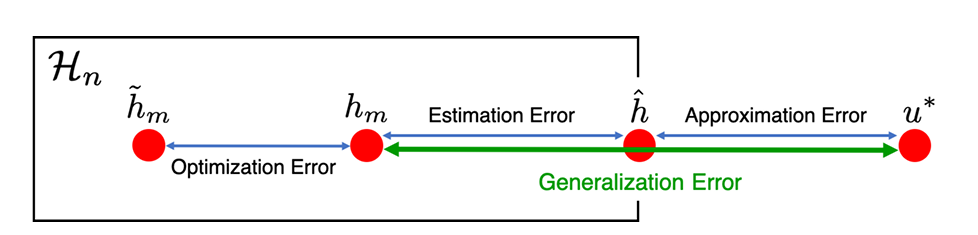
\includegraphics[width=0.75\linewidth]{shin_error_diagram.png}
  \caption[Errors that appear when training a PINN]{Diagram of the different errors that appear when training a PINN: optimization,
  estimation and approximation errors.}
  \label{fig:shin-errors}
  \fuente{Shin et al.~\cite{shin2020convergence}.}
\end{figure}
\verificar{permission / ``adapted from'' for the reproduced figure}

% =====================================================================
\section{Modern Theory of PINNs}\label{sec:pinn-theory}
% =====================================================================

This section collects the results that bound each of the three errors. We do not prove them; the goal
is to understand what each one says about our experiments. The theorem numbers refer to the original
works.\verificar{theorem/lemma numbers against the published versions}

% ---------------------------------------------------------------------
\subsection{Error Decomposition}

\begin{teorema}{Error decomposition \cite[Lemma~3.1 and Eq.~3.11]{deryck2022generic,deryck2024acta}.}\label{thm:error-decomp}
Suppose that the PDE is stable in the sense that $\norm{u-u_\theta}_X\le C\,\mathcal{E}_G(\theta)^{\alpha}$
for some $C,\alpha>0$, and let $\hat\theta$ be the parameter of the ideal model. Then the total error
$\mathcal{E}^{*}=\norm{u-u_{\theta^{*}(\T)}}_X$ satisfies
\[
  \mathcal{E}^{*}\le C\Big(\underbrace{\mathcal{E}_G(\hat\theta)}_{\text{approximation}}
  +\underbrace{2\sup_{\theta\in\Theta}\abs{\mathcal{E}_T(\theta;\T)-\mathcal{E}_G(\theta)}}_{\text{generalization gap}}
  +\underbrace{\mathcal{E}_T(\theta^{*}(\T);\T)-\mathcal{E}_T(\hat\theta;\T)}_{\text{optimization}}\Big)^{\alpha}.
\]
\end{teorema}

The stability hypothesis is exactly where the PDE theory of Chapter~\ref{ch:pdes} enters: for elliptic and
parabolic problems it follows from coercivity and the maximum principle; for hyperbolic problems it
follows from energy estimates (Section~\ref{subsec:energy-estimate}).

% ---------------------------------------------------------------------
\subsection{Approximation Error}

\begin{teorema}{Approximation with $\tanh$ networks \cite[Theorem~4.4]{deryck2021tanh}.}\label{thm:tanh-approx}
Let $\Omega=[0,1]^d$. For every $N\in\mathbb{N}$ and every $f\in W^{s,\infty}(\Omega)$ there exists a network
with $\tanh$ activation, two hidden layers and width $N$, $\hat u$, such that for all $0\le k<s$
\[
  \norm{f-\hat u}_{W^{k,\infty}(\Omega)}\le C\big(\ln(cN)\big)^{k}N^{-(s-k)/d}.
\]
\end{teorema}

\emph{Consequence.} The network approximates not only $f$ but also its derivatives up to order $k$, which
are the ones demanded by the operator $\mathcal{D}$. The rate, however, deteriorates with the dimension
$d$.

\begin{teorema}{Sobolev--Barron approximation \cite[Theorem~4.33]{deryck2024acta}.}\label{thm:barron}
Let $\sigma$ be smooth with $C_1:=\max_{m\le\ell}\norm{\sigma^{(m)}}_{L^\infty(\mathbb{R})}<\infty$. If $f$
belongs to the spectral Barron space $\mathcal{B}^{R}_{1}(\Omega)$ (index 1, radius $R\ge1$), then for
every width $k\in\mathbb{N}$ there exists a shallow network
$u_k(\mathbf{x})=\frac1k\sum_{i=1}^{k}a_i\sigma(\mathbf{w}_i^{\top}\mathbf{x}+b_i)$ with
$(a_i,\mathbf{w}_i,b_i)\in\mathbb{R}\times B^d_R\times\mathbb{R}$ such that
\[
  \norm{u_k-f}_{H^{\ell}_{\mu}(\Omega)}\le\frac{2C_1\big(R\sqrt{ed}\big)^{\ell}\norm{f}_{\mathcal{B}^R_1(\Omega)}}{\sqrt{k}}.
\]
\end{teorema}

The rate $k^{-1/2}$ is independent of $d$: in the Sobolev--Barron regime the network overcomes the
curse of dimensionality. Notice that the activation function only enters through the constant $C_1$,
the maximum of its derivatives up to the order $\ell$ of the PDE. We will use this observation to
analyze our adaptive activations in Section~\ref{sec:mabur}.

% ---------------------------------------------------------------------
\subsection{Generalization Gap}

\begin{teorema}{Generalization gap \cite[Theorem~6.2]{deryck2022kolmogorov,beck2022}.}\label{thm:generalization}
Let $\T$ consist of $N$ points drawn i.i.d.\ according to a measure $\mu$, let $\Theta=[-R,R]^{n}$ be
compact, and let $\mathfrak{L}$ be the Lipschitz constant of the map $\theta\mapsto\mathcal{E}_G(\theta)^2$.
Then
\[
  \mathbb{E}\big[\mathcal{E}_G(\theta^{*}(\T))^2\big]\le\mathbb{E}\big[\mathcal{E}_T(\theta^{*}(\T);\T)^2\big]
  +\sqrt{\frac{2c^2(n+1)}{N}\ln\Big(\frac{R\,\mathfrak{L}\sqrt{N}}{c}\Big)}.
\]
\end{teorema}

The average gap between the training and the generalization errors is of order
\[
  \mathcal{O}\Big(\frac{K_1}{\sqrt N}\ln\big(K_2\sqrt N\big)\Big).
\] For our experiments this means that the number
of collocation points must grow with the number of parameters $n$; this is one of the reasons for the
stochastic resampling of Section~\ref{subsec:sampling}, which shows the network new points at every epoch.

% ---------------------------------------------------------------------
\subsection{Optimization: Conditioning and Spectral Bias}

\begin{teorema}{Convergence in the NTK regime \cite[Theorem~7.9]{deryck2024operator}.}\label{thm:ntk-conv}
In the neural tangent kernel (NTK) regime (wide, over-parameterized networks), the number of gradient
descent steps needed to reduce the error to $\epsilon$ is
\[
  N(\epsilon)=\mathcal{O}\big(\kappa(A)\ln(1/\epsilon)\big),\qquad\kappa(A)=\frac{\lambda_{\max}(A)}{\lambda_{\min}(A)},
\]
with
$A_{ij}=\langle\mathcal{D}\varphi_i,\mathcal{D}\varphi_j\rangle_{L^2(\Omega)}+\lambda\langle\varphi_i,\varphi_j\rangle_{L^2(\partial\Omega)}$
and $\varphi_i(\mathbf{x})=\nabla_{\theta_i}u_\theta(\mathbf{x};\theta_0)$.
\end{teorema}

\begin{teorema}{Spectral bias and conditioning \cite[Theorem~7.10]{deryck2024operator}.}\label{thm:spectral-bias}
$\kappa(A)$ is governed by the condition number of the operator $\mathcal{A}\circ TT^{*}$, where
$\mathcal{A}=\mathcal{D}^{*}\mathcal{D}$ and $TT^{*}$ is the integral operator whose kernel is associated
with the architecture.
\end{teorema}

\emph{Pathology of conditioning.} Since $\mathcal{D}^{*}\mathcal{D}$ contains derivatives of twice the
order of the PDE, high frequencies make $\kappa(A)$ blow up rapidly: a Fourier mode $e^{ikx}$ is
amplified by a factor of order $k^{4}$ for a second-order operator. For the Klein--Gordon operator,
$\mathcal{D}^{*}\mathcal{D}$ multiplies the mode $e^{i(kx-\omega t)}$ by $(\omega^2-k^2-m^2)^2$, which
is why initial conditions with several wavenumbers are a hard test.

\paragraph{Spectral convergence rate.}
In the theory of Jacot et al.~\cite{jacot2018} and its extension to PINNs by Wang et al.~\cite{wang2022ntk}, it is shown
that, under an infinitesimal learning rate, the evolution in training time $\tau$ of the vector of
predictions $\mathbf{f}_\theta(\tau)$ with respect to the targets $\mathbf{Y}$ satisfies the linear ODE
\begin{equation}
  \frac{\,d\mathbf{f}_\theta(\tau)}{\,d\tau}\approx-\mathbf{K}\big(\mathbf{f}_\theta(\tau)-\mathbf{Y}\big),
  \label{eq:ntk-ode}
\end{equation}
where $\mathbf{K}$ is the NTK. Projecting the error onto the eigenvectors $\mathbf{q}_i$ of $\mathbf{K}$,
with eigenvalues $\lambda_i$, we obtain the analytical solution
\begin{equation}
  \mathbf{q}_i^{T}\big(\mathbf{f}_\theta(\tau)-\mathbf{Y}\big)=e^{-\lambda_i\tau}\,\mathbf{q}_i^{T}\big(\mathbf{f}_\theta(0)-\mathbf{Y}\big).
  \label{eq:ntk-modes}
\end{equation}
The components of the error associated with large eigenvalues (low frequencies, for standard MLPs)
are learned first, while those associated with small eigenvalues (high frequencies) are learned
exponentially slower. This is the spectral bias, and it is the counterpart, inside the optimizer, of
the parabolic decay $e^{-\lambda_k t}$ of Equation~\eqref{eq:parabolic-modes}: the network ``diffuses'' its error
mode by mode.

% ---------------------------------------------------------------------
\subsection{Regularized Loss and the Hölder Seminorm}

For linear second-order elliptic and parabolic PDEs, Shin et al.~\cite{shin2020convergence} proved that the
PINN loss with $m_r$ residual points and $m_b$ boundary points satisfies
\begin{equation}
  \mathrm{Loss}^{\mathrm{PINN}}(h;\lambda)\le C_m\cdot\mathrm{Loss}_m(h;\lambda,\hat\lambda^{R}_m)
  +C'\big(m_r^{-\alpha/d}+m_b^{-\alpha/(d-1)}\big),
  \label{eq:shin-bound}
\end{equation}
where $\mathrm{Loss}^{\mathrm{PINN}}_m(h;\lambda)=\Loss(\theta)$, $h$ denotes the functions involved
($u_\theta$, $\partial_t u_\theta$, $\mathcal{D}[u_\theta]$), and $\lambda,\hat\lambda$ are the
coefficients of the loss function.\verificar{exponents of $m_r$ and $m_b$ against the original}
This tells us that if we reduce the loss function and the values $m_r^{-\alpha/d}$ and
$m_b^{-\alpha/(d-1)}$, it is possible to find a good estimation. The bound applies to a loss that is
regularized through the Hölder seminorm,
\begin{equation}
  \mathrm{Loss}_m(h;\lambda,\hat\lambda^{R}_m)=\mathrm{Loss}^{\mathrm{PINN}}_m(h;\lambda)
  +\hat\lambda^{R}_f[\mathcal{R}_f[h]]^2_{\alpha;U}+\hat\lambda^{R}_{bc}[\mathcal{R}_{bc}[h]]^2_{\alpha;U}
  +\hat\lambda^{R}_{ic}[\mathcal{R}_{ic}[h]]^2_{\alpha;U},
  \label{eq:shin-regularized}
\end{equation}
where $\mathcal{R}_i$ are the residuals of Equations~\eqref{eq:res-pde}--\eqref{eq:res-ic1} and the Hölder seminorm
(Definition~\ref{def:holder-norm}) is
\begin{equation}
  [\mathcal{R}_i[h]]_{\alpha;U}=\sup_{\substack{\mathbf{x},\mathbf{y}\in U\\ \mathbf{x}\neq\mathbf{y}}}
  \frac{\norm{\mathcal{R}_i[h](\mathbf{x})-\mathcal{R}_i[h](\mathbf{y})}}{\norm{\mathbf{x}-\mathbf{y}}^{\alpha}},\qquad0<\alpha\le1.
  \label{eq:holder-seminorm-loss}
\end{equation}
It is natural to try to regularize the loss function through $L^1$ or $L^2$ penalties of the
parameters; however, this does not make the network represent the behavior of the solution more
faithfully. The Hölder regularization is different: it penalizes the oscillation of the residual, and it
assumes that the unknown residuals are Hölder continuous, which is the kind of uniform equicontinuity
needed to pass from the discrete loss to the continuous one. The proof of Shin et al.~\cite{shin2020convergence}
uses the regularity estimates and the maximum principle of elliptic and parabolic equations. As we saw
in Section~\ref{sec:regularity-bridge}, hyperbolic PDEs have particularities, such as not having a maximum
principle, which does not allow us to find a convergence bound in the same way. A natural alternative is
to work with the energy conservation that this type of equation satisfies.

% ---------------------------------------------------------------------
\subsection{Energy Estimate for the Klein--Gordon Equation}\label{subsec:energy-estimate}\label{sec:energy-estimate}

Since the Klein--Gordon equation is dispersive and conservative, the energy must be conserved
(Equation~\eqref{eq:kg-energy}). This allows an energy analysis in Sobolev spaces and, therefore, an extension
of Equation~\eqref{eq:shin-regularized} with a term coming from the energy. The estimate for the error is computed
through the error $e=u_\theta-u$, which, by linearity, satisfies the same operator with the residual as
source:
\begin{equation}
  \partial_{tt}e-\nabla^2e+m^2e=r\quad\text{in }\Omega\times(0,T),\qquad
  e(\cdot,0)=I_0,\quad\partial_te(\cdot,0)=I_1,\quad e|_{\partial\Omega}=B,
  \label{eq:error-pde}
\end{equation}
where $r=R_{\mathrm{PDE}}$, $I_0=R_{ic0}$, $I_1=R_{ic1}$ and $B=R_{bc}$ are the residuals of
Equations~\eqref{eq:res-pde}--\eqref{eq:res-ic1}. The energy of the error is
\begin{equation}
  E(t)=\frac12\int_\Omega\Big(\abs{\partial_te}^2+\abs{\nabla e}^2+m^2\abs{e}^2\Big)\,d\mathbf{x}.
  \label{eq:error-energy}
\end{equation}

\begin{teorema}{Energy estimate for the PINN error.}\label{thm:energy-estimate}
Let $e$ be a sufficiently smooth solution of Equation~\eqref{eq:error-pde}. Then, for all $t\in[0,T]$,
\begin{equation}
  E(t)\le\Big(E(0)+\frac12\int_0^t\Big[\norm{r}^2_{L^2(\Omega)}+\norm{\partial_tB}^2_{L^2(\partial\Omega)}
  +\Big\|\frac{\partial e}{\partial\mathbf{n}}\Big\|^2_{L^2(\partial\Omega)}\Big]\,d s\Big)e^{t},
  \label{eq:energy-bound}
\end{equation}
with initial energy
$E(0)=\frac12\big(\norm{I_1}^2_{L^2}+\norm{\nabla I_0}^2_{L^2}+m^2\norm{I_0}^2_{L^2}\big)$.
\end{teorema}

The proof (Appendix~\ref{app:energy}) uses integration by parts, Young's inequality and Gronwall's inequality.
The bound says that the energy of the error is controlled by the initial energy of the error, plus the
accumulated residual, plus the accumulated error flux through the boundary, times an amplification
factor. Each of these terms can be approximated by the loss functions
Equations~\eqref{eq:loss-f}--\eqref{eq:loss-bc}, weighted by the coefficients of the learning rate annealing
(Section~\ref{subsec:lra}), except two of them: the initial energy needs the \emph{gradient} of the initial
position residual, $\norm{\nabla I_0}^2_{L^2}$, which a standard PINN does not penalize, and the boundary
needs $\partial_tB$ and the normal flux of the error. Therefore, to control the energy of the error, the
loss must include the term $\norm{\nabla I_0}^2_{L^2}$ (and $\norm{\partial_tB}^2$ for non-periodic
boundaries). For periodic boundary conditions, as in our experiments, the boundary terms cancel and this
part of the regularization is not necessary. In one spatial dimension, $E(t)\to0$ implies convergence
in $H^1$ and, by the Sobolev embedding $H^1\subset C^{0,1/2}$, uniform convergence.

\begin{remarkbox}[Remark (which residual gradients are needed)]
One could think that the gradients of all residuals,
$\{\norm{\nabla B},\norm{\nabla I_0},\norm{\nabla I_1},\norm{\nabla r}\}$, must be added to the loss.
The estimate \eqref{eq:energy-bound} only requires $\nabla I_0$ (and $\partial_tB$); the terms
$\nabla I_1$ and $\nabla r$ would be needed for a higher-order energy (controlling $\partial_t\nabla e$
and $\nabla^2e$), and $\nabla r$ is costly because it needs third derivatives of $u_\theta$, as in
gradient-enhanced PINNs \cite{yu2022gpinn}. This is consistent with Experiment~2
(Section~\ref{sec:exp-regularization}), where adding derivative regularization did not improve the error.
\end{remarkbox}

% =====================================================================
\section{The Optimization Problem: Hard vs.\ Soft Constraints}\label{sec:optimization}
% =====================================================================

The formulation of the PINN problem can be rigorously analyzed through the lens of constrained
optimization. If we wish to minimize the data loss subject to the strict constraint that the physics
loss is zero, we formulate a minimization with an equality constraint (hard constraint)
\cite{krishnapriyan2021}:
\begin{align}
  \min_{\theta}\ &\Loss_{ic}(\theta)+\Loss_{bc}(\theta), \label{eq:hard-obj}\\
  \text{s.t. }\ &\Loss_f(\theta)=0. \label{eq:hard-constraint}
\end{align}
According to Krishnapriyan et al.~\cite{krishnapriyan2021}, this problem is costly to solve. To see why, we introduce the
Lagrangian function with the dual variable $v\in\mathbb{R}$:
\begin{equation}
  \mathscr{L}(\theta,v)=\Loss_{\mathrm{data}}(\theta)+v\,\Loss_f(\theta)
  =\big(\Loss_{ic}(\theta)+\Loss_{bc}(\theta)\big)+v\,\Loss_f(\theta).
  \label{eq:lagrangian}
\end{equation}
The Karush--Kuhn--Tucker (KKT) conditions for this system are \cite{boyd2004}
\begin{align}
  \nabla_\theta\Loss_{ic}(\theta^{*})+\nabla_\theta\Loss_{bc}(\theta^{*})+v\nabla_\theta\Loss_f(\theta^{*})&=0, \label{eq:kkt-1}\\
  \Loss_f(\theta^{*})&=0. \label{eq:kkt-2}
\end{align}
Expanding these gradients (Appendix~\ref{app-sec:kkt-gradients}), the gradients of the initial and boundary
terms contain $2u_\theta\nabla_\theta u_\theta$ and $2g_0\nabla_\theta u_\theta$, which are nonlinear in
$\theta$, because $u_\theta$ is nonlinear and so is its derivative. For the physics loss, the gradient is
even more complex because of the differential operator: for the Klein--Gordon operator
$\mathcal{D}_{KG}=\partial_{tt}-\nabla^2+m^2$ it requires differentiating with respect to the parameters
through the temporal and spatial derivatives of the network ($\partial_{tt}$, $\nabla^2$), which increases
the computational complexity compared with a standard neural network. Written in matrix form, the KKT
conditions are a system of high-dimensional nonlinear equations, where the dimensionality is induced by
the neural network.

\paragraph{A degenerate constraint.}
There is a subtle problem with Equation~\eqref{eq:hard-constraint}. Since $\Loss_f\ge0$, every feasible point
($\Loss_f(\theta^{*})=0$) is a global minimizer of $\Loss_f$, and therefore $\nabla_\theta\Loss_f(\theta^{*})=0$.
The gradient of the only constraint vanishes at every feasible point, so the usual constraint
qualification (linear independence of the constraint gradients) fails, and the KKT conditions are not
guaranteed to characterize the optimum.\verificar{add a reference on constraint qualifications, e.g.\
Nocedal \& Wright} This suggests that there should be one Lagrange multiplier per constraint, that is,
one per collocation point (Appendix~\ref{app-sec:kkt-gradients}); whether that system has a solution
presupposes that the chosen architecture has enough features to give existence to that optimal point.

\paragraph{Non-convexity.}
To analyze the convexity of the loss functions, one should compute the Hessian of each loss function
$\nabla^2_\theta\Loss_i(\theta)$ and its eigenvalues (Appendix~\ref{app-sec:nonconvexity}). The Hessian has
a Gauss--Newton part, which is always positive semidefinite, and a second part that contains the
residual times $\nabla^2_\theta u_\theta$, whose sign is not known. Already for a single layer the
dependence on the parameters passes through an activation that is neither convex nor concave, so the
cost function is non-convex, and non-convex optimization methods must be used.

\paragraph{Computational cost of Newton's method.}
Since $\Loss_{\mathrm{data}}$ and $\Loss_f$ are not convex, and we do not know where the feasible region
is, Boyd and Vandenberghe~\cite{boyd2004} suggest the infeasible-start Newton method, which applies the Newton step
$\nabla^2\mathscr{L}\,\delta=-\nabla\mathscr{L}$ to both variables $(\theta,v)$ with the linearized
constraint (Appendix~\ref{app-sec:newton}).
Applying this method consumes significant computational resources, because it must compute the Hessian
of the approximating function $u_\theta$ for the losses of the initial and boundary data, and the
Hessian of the physics loss, which in turn contains spatial and temporal derivatives of $u_\theta$. To
estimate the cost, recall that the universal approximation theorem says that a large enough network
can approximate a function with any desired accuracy, but not how large \cite{lecun2015}, and that
deep networks can represent certain families of functions with exponentially fewer units than shallow
ones \cite{delalleau2011}; so the PINN should be deep as well as wide. For the architecture of
Wang et al.~\cite{wang2021gradient}, with $50$ neurons per layer and $6$ hidden layers, each layer has
$50\times50$ weights plus $50$ biases, that is, $2\,550$ parameters, and the network has about
$6\times2\,550=15\,300$ parameters (ignoring the input and output layers). The Hessian has
$P^2\approx2.34\times10^{8}$ entries, which in single precision is close to one gigabyte of memory, at
every iteration. Moreover, Wang et al.~\cite{wang2021gradient} observed that the eigenvalues of the Hessian of
the physics loss are very dispersed (very ill-conditioned), so Newton's method would need many
iterations to satisfy the physics. As a result, the hard-constrained approach is intractable at scale.

% ---------------------------------------------------------------------
\subsection{Soft Constraints and Multi-Objective Optimization}

Therefore, the hard constraint is relaxed into a soft constraint: a regularization constant is placed in
the objective function, which transforms the constrained problem into an unconstrained multi-objective
(MO) problem \cite{krishnapriyan2021}. To understand what is lost, recall the vector optimization
problem of Boyd and Vandenberghe~\cite{boyd2004}:
\begin{equation}
  \text{minimize (w.r.t. } K)\ \ f_0(\mathbf{x})\qquad\text{s.t. } f_i(\mathbf{x})\le0,\ \ h_j(\mathbf{x})=0,
  \label{eq:vector-opt}
\end{equation}
where $\mathbf{x}\in\mathbb{R}^n$ is the optimization variable, $f_0:\mathbb{R}^n\to\mathbb{R}^q$ is the vector objective,
$K\subseteq\mathbb{R}^q$ is a proper cone ($K=\mathbb{R}^q_+$ in our case), $f_i$ are the inequality constraints and
$h_j$ the equality constraints. The set of achievable objective values is
\begin{equation}
  \mathcal{O}=\{f_0(\mathbf{x})\mid\exists\,\mathbf{x}\in\mathcal{D},\ f_i(\mathbf{x})\le0,\ i=1,\dots,m;\ h_j(\mathbf{x})=0,\ j=1,\dots,p\}.
  \label{eq:achievable-set}
\end{equation}
A feasible point $\mathbf{x}^{*}$ is optimal if its objective can be compared with that of every other feasible
point and is better or equal, that is, $\mathcal{O}\subseteq f_0(\mathbf{x}^{*})+K$. The set $f_0(\mathbf{x}^{*})+K$ is
the cone centered at $f_0(\mathbf{x}^{*})$ that defines the order relation: it points to where the worse results
are. If $K$ points to the worse results, then $-K$ points to the better ones; that is, if we stand at
$f_0(\mathbf{x}^{*})$, look in the direction $-K$ and see no other achievable value of $\mathcal{O}$, then we are at
a \emph{Pareto optimal} value. The Pareto optimal values are minimal elements of $\mathcal{O}$, and they
lie on its boundary,
\begin{equation}
  \mathcal{P}\subseteq\mathcal{O}\cap\operatorname{bd}\mathcal{O}.
  \label{eq:pareto}
\end{equation}
In this way, we introduce the minimization problem of Krishnapriyan et al.~\cite{krishnapriyan2021}:
\begin{equation}
  \min_{\theta}\ \Loss_{ic}(\theta)+\Loss_{bc}(\theta)+\lambda_f\Loss_f(\theta).
  \label{eq:soft}
\end{equation}
If $\lambda_f=1$, this is what is known as the \emph{vanilla PINN}. Here, a weight vector
$\lambda\succeq_{K^{*}}0$ represents a supporting hyperplane of $\mathcal{O}$ at the optimum found, which is
the point of contact. This presupposes a problem: if the set $\mathcal{O}$ is not convex, there are Pareto
values in the regions that cannot be supported by a hyperplane, so the scalarization will not find all
the Pareto points, but only some of them that also minimize the objective function. The formulation of
the optimization problem can be generalized further \cite{rohrhofer2023}:
\begin{equation}
  \min_{\theta}\sum_{i\in\{f,ic,bc\}}\lambda_i\Loss_i(\theta).
  \label{eq:soft-general}
\end{equation}
If $\lambda_f=1$, this is the loss function proposed by Wang et al.~\cite{wang2021gradient}, which weights the
data losses with respect to the physics loss:
\begin{equation}
  \min_{\theta}\ \Loss_f(\theta)+\sum_{i\in\{ic,bc\}}\lambda_i\Loss_i(\theta).
  \label{eq:soft-wang}
\end{equation}
In this way, a balance between the gradients of the data and physics losses is sought, preventing one
term from governing the other. Rohrhofer et al.~\cite{rohrhofer2023} named the related phenomenon the \emph{apparent
Pareto front}: gradient methods (Newton, ADAM, SGD, etc.) reach a set of locally optimal trade-offs
between the loss terms, which is the same gradient problem found by Wang et al.~\cite{wang2021gradient}.

% =====================================================================
\section{Gradient Pathologies and Optimizers}\label{sec:gradient-pathologies}
% =====================================================================

Training a PINN involves navigating a highly non-convex and stiff loss landscape. For
Equation~\eqref{eq:soft-wang} the only KKT condition is the first-order condition for local optima,
\begin{equation}
  \underbrace{\nabla_\theta\big(\lambda_{ic}\Loss_{ic}(\theta)+\lambda_{bc}\Loss_{bc}(\theta)\big)}_{\text{gradient of the data}}
  =\underbrace{-\nabla_\theta\Loss_f(\theta)}_{\text{gradient of the physics}},
  \label{eq:kkt-soft}
\end{equation}
so at a stationary point the two gradients must be equal in magnitude and opposite in direction. If
$\lambda_{ic}=\lambda_{bc}=1$, we have the problem of gradient imbalance: the gradients coming from the
PDE loss ($\nabla_\theta\Loss_f$) are usually larger and stiffer than those coming from the initial and
boundary conditions ($\nabla_\theta\Loss_i$). Because ADAM attempts to minimize the global error, it
dedicates most of its effort to the term with the largest gradient, that is, the gradient that governs
the cost function \cite{wang2021gradient}.

% ---------------------------------------------------------------------
\subsection{Stiffness Analysis}

To analyze this stiffness, Wang et al.~\cite{wang2021gradient} used the loss function of the vanilla PINN and
the steepest descent method,
\begin{equation}
  \theta_{n+1}=\theta_n-\eta\nabla_\theta\Loss(\theta_n)=\theta_n-\eta\big(\nabla_\theta\Loss_f(\theta_n)+\nabla_\theta\Loss_{\mathrm{data}}(\theta_n)\big),
  \label{eq:gd}
\end{equation}
where $\eta$ is the learning rate (the step). They apply a Taylor expansion of the loss function around the current parameters, up to second order,
and diagonalize the Hessian $\nabla^2_\theta\Loss(\xi)=Q^{T}\diag(\lambda_1,\dots,\lambda_P)Q$ by the
spectral theorem \cite{trefethen1997}. With $\mathbf{y}=Q\nabla_\theta\Loss(\theta_n)/\norm{\nabla_\theta\Loss(\theta_n)}$
(Appendix~\ref{app-sec:stiffness}), the loss difference after one step becomes
\begin{equation}
  \Loss(\theta_{n+1})-\Loss(\theta_n)=\eta\norm{\nabla_\theta\Loss(\theta_n)}^2
  \Big(-1+\frac12\eta\sum_{i=1}^{P}\lambda_iy_i^2\Big).
  \label{eq:stiffness}
\end{equation}
For the optimization method to work, we want $\Loss(\theta_{n+1})<\Loss(\theta_n)$, so the term in
parentheses must be negative, which requires $1>\frac12\eta\sum_i\lambda_iy_i^2$. This is only possible if
the eigenvalues are small (the loss function near the minimum is smooth and well behaved); if the
landscape is complicated, the eigenvalues are large and, instead of following the descent path, the
iterate jumps away to another valley. Decomposing the loss into its objectives, the same procedure gives
\begin{equation}
  \Loss_j(\theta_{n+1})-\Loss_j(\theta_n)\approx\eta\norm{\nabla_\theta\Loss_j(\theta_n)}^2
  \Big(-1+\frac12\eta\sum_{i=1}^{P}\lambda^{j}_i(y^{j}_i)^2\Big),\qquad j\in\{f,ic,bc\},
  \label{eq:stiffness-split}
\end{equation}
where $\lambda^{j}_i$ are the eigenvalues of $\nabla^2_\theta\Loss_j$. According to
Wang et al.~\cite{wang2021gradient}, the cause of the gradient imbalance is in the eigenvalues $\lambda^{f}_i$
associated with the physics loss, which are very large near a minimum.

Moreover, Wang et al.~\cite{wang2021gradient} bound the size of each gradient by the largest eigenvalue of
the curvature of its loss (Appendix~\ref{app-sec:grad-bounds}), which reaffirms the imbalance between
gradients.

% ---------------------------------------------------------------------
\subsection{Learning Rate Annealing}\label{subsec:lra}

To mitigate this, learning rate annealing (LRA) is used to dynamically balance the gradients
\cite{wang2021gradient}. We start from the objective \eqref{eq:soft-wang} and minimize it with a
first-order method:
\begin{equation}
  \theta_{n+1}=\theta_n-\eta\Big(\nabla_\theta\Loss_f(\theta_n)+\sum_{i\in\{ic,bc\}}\lambda_i\nabla_\theta\Loss_i(\theta_n)\Big).
  \label{eq:lra-update}
\end{equation}
The weights of the initial and boundary losses are computed as
\begin{equation}
  \hat\lambda_i=\frac{\max_\theta\abs{\nabla_\theta\Loss_f(\theta_n)}}{\overline{\abs{\nabla_\theta\Loss_i(\theta_n)}}},
  \label{eq:lra-weights}
\end{equation}
where the numerator is the maximum (over the components of $\theta$) of the gradient of the physics loss
and the denominator is the mean of the absolute gradient of the loss $i$.\verificar{whether the
denominator includes $\lambda_i$, as in the original Algorithm~1} By using the maximum, the numerator
captures the largest stiffness of the differential equation, acting as an upper limit that represents the
worst-case scenario, while the average in the denominator works as a regularizer. A general analysis of
the possible situations gives:
\begin{itemize}
  \item If $\hat\lambda_i\approx1$, the worst-case gradient of the physics and the average gradient of
    the data term $i$ have the same magnitude: the gradients are balanced and no reweighting is needed.
  \item If $\hat\lambda_i>1$ (the usual situation), the physics gradient dominates, and the weight of
    the term $i$ is increased so that the optimizer does not neglect it; geometrically, the
    scalarization moves to another region of the (apparent) Pareto front.
  \item If $\hat\lambda_i<1$, the average gradient of the data term $i$ is larger than the worst case of
    the physics gradient, and its weight is decreased, giving room to the physics.
\end{itemize}
The weights are then updated with an exponential moving average to remove the noise generated by the
stochastic gradients during training:
\begin{equation}
  \lambda_i\leftarrow(1-\alpha)\lambda_i+\alpha\hat\lambda_i.
  \label{eq:lra-ema}
\end{equation}
The algorithm proposed by Wang et al.~\cite{wang2021gradient} is given in Algorithm~\ref{alg:lra}, with the modification
of using ADAM instead of plain gradient descent.

\begin{algorithm}[htbp]
  \caption{Learning rate annealing with ADAM.}
  \label{alg:lra}
  \begin{algorithmic}[1]
    \Require Recommended hyperparameters $\eta=10^{-3}$, $\alpha=0.9$; number of steps $S$; number of
      constraint terms $M$; initial weights $\lambda_i$, $i=1,\dots,M$.
    \For{$n=1$ to $S$}
      \State \textit{(a) Gradient statistics}
      \State $G_{\max}\gets\max_\theta\{\abs{\nabla_\theta\Loss_f(\theta_n)}\}$ \Comment{maximum gradient of the physics residual}
      \State $G^{i}_{\mathrm{mean}}\gets\overline{\abs{\nabla_\theta\Loss_i(\theta_n)}}$ for each term $i$
      \State $\hat\lambda_i\gets G_{\max}/G^{i}_{\mathrm{mean}}$ \Comment{Equation~\eqref{eq:lra-weights}}
      \State \textit{(b) Weight update (moving average)}
      \State $\lambda_i\gets(1-\alpha)\lambda_i+\alpha\hat\lambda_i$ \Comment{Equation~\eqref{eq:lra-ema}}
      \State \textit{(c) Network parameters update}
      \State $\nabla_{\mathrm{total}}\gets\nabla_\theta\Loss_f(\theta_n)+\sum_{i=1}^{M}\lambda_i\nabla_\theta\Loss_i(\theta_n)$
      \State $\theta_{n+1}\gets\mathrm{ADAM}(\theta_n,\nabla_{\mathrm{total}},\eta)$ \Comment{Equation~\eqref{eq:adam}}
    \EndFor
    \State \Return optimized parameters $\theta_{S+1}$
  \end{algorithmic}
\end{algorithm}

% ---------------------------------------------------------------------
\subsection{ADAM as an Approximation of the Natural Gradient}

To understand the ADAM method, one can start from the natural gradient
\cite{amari1998,pascanu2013}. This means that the step no longer moves through the common Euclidean
space of parameters, but through the space of probability distributions, under the metric induced by
the Kullback--Leibler (KL) divergence. For this, the Fisher information matrix $F$ is introduced in the
gradient descent method:
\begin{equation}
  \theta_{n+1}=\theta_n-\eta\,F^{-1}\nabla_\theta\Loss(\theta_n),\qquad
  F=\mathbb{E}\big[\nabla_\theta\log P(\mathbf{x}\mid\theta)\,\nabla_\theta\log P(\mathbf{x}\mid\theta)^{T}\big].
  \label{eq:natural-gradient}
\end{equation}
The Fisher matrix is the second moment of $\nabla_\theta\log P(\mathbf{x}\mid\theta)$, which looks like the
gradient of a typical loss function for a likelihood \cite{amari1998}; it contains the variances and
covariances of the stochastic steps generated by the mini-batches, and it is the local quadratic
approximation of the KL divergence, $\mathrm{KL}(\theta\,\|\,\theta+\delta)\approx\frac12\delta^{T}F\delta$
(Appendix~\ref{app:fisher}). The ADAM method assumes, in practice, that the parameters are independent of each
other, so only the diagonal elements of the Fisher matrix survive. In addition, ADAM keeps the exponential
decay of the momentum method \cite{ruder2016} for the first moment, and it adds the second moment as
a proxy of the diagonal of the Fisher matrix \cite{kingma2015}:
\begin{equation}
  \begin{gathered}
  \theta_{n+1}=\theta_n-\eta\frac{\hat m_n}{\sqrt{\hat v_n}+\epsilon},\\
  m_n=\beta_1m_{n-1}+(1-\beta_1)\nabla_\theta\Loss(\theta_n),\qquad
  v_n=\beta_2v_{n-1}+(1-\beta_2)\big(\nabla_\theta\Loss(\theta_n)\big)^2,
  \end{gathered}
  \label{eq:adam}
\end{equation}
where $\hat m_n,\hat v_n$ are the bias-corrected moments. Kingma and Ba~\cite{kingma2015} explain that they use the
square root of the inverse of the variance because it preserves invariance to the scale of the gradient
and it is a more conservative preconditioner. In the natural gradient method, if the Fisher curvature is
small, the method assumes that it is in a flat basin and takes a very large step to cross it; since our
functions are non-convex, this can skip local minima. To mitigate this, ADAM does not use the whole
variance, but its square root, something like a standard deviation. We must say that, for a PINN loss
(which is not a likelihood), this analogy is heuristic; the recent natural-gradient methods for PINNs
\cite{schwencke2025anagram,schwencke2025thesis} make it precise by using the metric of the model in
function space.

\paragraph{Second-order refinement (L-BFGS).}
After ADAM with LRA has found a region of the parameter space where a good trade-off between losses is
located, a quasi-Newton method can be used as a final minimizer. L-BFGS builds an approximation of the
inverse Hessian from the last pairs of differences of parameters and gradients, so it uses curvature
information without storing the $P\times P$ Hessian.\verificar{add reference for L-BFGS (Liu \& Nocedal,
1989)} We use it in the preliminary experiment of Section~\ref{sec:exp-preliminary}.

% =====================================================================
\section{Training Strategies for Hyperbolic PDEs}\label{sec:training-strategies}
% =====================================================================

Until now we have attacked the gradient stiffness, which induces the optimizer to fall into local minima;
however, we have not attacked the specific problems of hyperbolic PDEs, such as the propagation of wave
fronts. Beyond optimization, specific techniques are required.

\paragraph{Causal training.}
Causal training puts a blindfold on the physics loss, forcing it to focus on the present before moving
to the future \cite{wang2024causality}. Since propagation phenomena depend on the past, the neural
network must respect this process. The time domain is divided into $N_t$ chunks $\{t_i\}$, and the
physics loss is weighted by a factor that depends on the residuals of the past:
\begin{equation}
  \Loss_f=\frac{1}{N_t}\sum_{i=1}^{N_t}w_i\Loss_f(\theta;t_i),\qquad
  w_i=\exp\Big(-\epsilon\sum_{k=1}^{i-1}\Loss_f(\theta;t_k)\Big).
  \label{eq:causal}
\end{equation}
This imposes a penalization factor $\epsilon$: the residual at time $t_i$ is only taken into account when
the residuals of all previous times are small. Wang et al.~\cite{wang2024causality} propose values
$\epsilon\in\{10^{-2},10^{-1},10^{0},10^{1},10^{2}\}$. Without this mechanism, the network can find
minima that satisfy the PDE but do not have physical meaning (for example, the trivial solution far from
$t=0$), that is, minima that deceive the network.

\paragraph{Focused stochastic sampling.}\label{subsec:sampling}
Since the domain is large and the computing time grows with the amount of data, a stochastic sampling
scheme is used: at each epoch, new sets of $N_f$, $N_{bc}$, $N_{ic}$ points are drawn. Because of the
gradient stiffness, more collocation points are assigned to the physics than to the initial and boundary
conditions. In dispersive equations, the wave fronts carry the most critical dynamics; the physics happens
inside these fronts, and the exterior must keep the initial (resting) state. For this reason, we designed
a localized scheme that assigns $80\%$ of the physics collocation points inside the light cone
$\{\abs{x}\le t\}$ (where the wave propagates, since the group velocity is bounded by $c=1$,
Equation~\eqref{eq:kg-group-velocity}) and $20\%$ outside, to guarantee that the network does not violate the physics
outside the cone.

\paragraph{Input normalization.}
Normalizing the variables allows comparing them on the same scale, ensuring a uniform contribution of each
input during training, which leads to more accurate results \cite{xu2025preprocessing}. We use a
modified min--max scaling to the range $[-1,1]$:
\begin{equation}
  x_{\mathrm{norm}}=2\frac{x-x_{\min}}{x_{\max}-x_{\min}}-1=\alpha_x(x-x_{\min})-1,\qquad
  t_{\mathrm{norm}}=2\frac{t-t_{\min}}{t_{\max}-t_{\min}}-1=\alpha_t(t-t_{\min})-1,
  \label{eq:normalization}
\end{equation}
with $\alpha_x=2/(x_{\max}-x_{\min})$ and $\alpha_t=2/(t_{\max}-t_{\min})$. Since the loss functions
express the physics in the original domain, the derivatives must be scaled by the chain rule,
$\partial_x=\alpha_x\partial_{x_{\mathrm{norm}}}$, $\partial_x^2=\alpha_x^2\partial^2_{x_{\mathrm{norm}}}$,
and analogously for $t$. The Klein--Gordon operator becomes
\begin{equation}
  \big(\alpha_t^2\partial_{tt}-\alpha_x^2\nabla^2+m^2\big)u_\theta(x_{\mathrm{norm}},t_{\mathrm{norm}})=0,
  \label{eq:kg-normalized}
\end{equation}
where the derivatives are taken with respect to the normalized variables.

% =====================================================================
\section{Representation: Fourier Features and Activation Functions}\label{sec:representation}
% =====================================================================

\paragraph{Random Fourier features.}
To overcome the spectral bias of MLPs (their tendency to learn low frequencies first,
Equation~\eqref{eq:ntk-modes}), transformations of the input coordinates based on Fourier features have been
proposed. The most common technique is random Fourier features \cite{tancik2020}, which apply the
mapping
\begin{equation}
  \gamma(\mathbf{v})=\begin{pmatrix}\cos(B\mathbf{v})\\ \sin(B\mathbf{v})\end{pmatrix},
  \label{eq:fourier-features}
\end{equation}
where each entry of $B\in\mathbb{R}^{m\times d}$ is sampled independently from $\mathcal{N}(0,\sigma^2)$. This mapping
modifies the spectrum of the NTK and allows fully connected networks to learn high frequencies more
effectively. In the context of PINNs, Wang et al.~\cite{wang2021eigenvector} extended this idea with multi-scale
Fourier embeddings to represent wave phenomena, taking advantage of the separability of variables: several
mappings with different values $\sigma_i$ are applied separately to the spatial and temporal coordinates;
the outputs of each branch enter a shallow but wide MLP, and the outputs are combined by point-wise
multiplication before the output layer. This strategy captures periodic or rapidly varying behaviors at
different scales, as shown in wave, reaction--diffusion and convection equations. The price is a new
hyperparameter, $\sigma$, whose value must be tuned for each problem.

\paragraph{Sinusoidal activations (SIREN).}
For training networks on periodic PDEs or on solutions that are approximated by Fourier series,
Sitzmann et al.~\cite{sitzmann2020} proposed the SIREN methodology, with sinusoidal activation functions:
\begin{equation}
  \Phi(\mathbf{x})=W_n(\varphi_{n-1}\circ\varphi_{n-2}\circ\dots\circ\varphi_0)(\mathbf{x})+\mathbf{b}_n,\qquad
  \varphi_i(\mathbf{x}_i)=\sin(\omega_0W_i\mathbf{x}_i+\mathbf{b}_i).
  \label{eq:siren}
\end{equation}
The authors argued that, when using SIREN, the initialization of the parameters must be adjusted, because
the sine is almost linear near zero: if the weights are initialized with very small values, the activation
loses its representation power. To fix this, they analyzed the distribution of the output signal of each
layer. At the input, the distribution is assumed uniform; after the sinusoidal activation the output
follows an arcsine distribution, and, after several layers, by the central limit theorem, the
pre-activations become normally distributed. To keep this distribution stable across layers they proposed
the initialization
\begin{equation}
  w_i\sim\mathcal{U}\Big(-\sqrt{6/n},\ \sqrt{6/n}\Big),
  \label{eq:siren-init}
\end{equation}
where $n$ is the number of inputs of the neuron, and a large factor $\omega_0$ that scales the frequencies
to attack the problem of small values (low frequencies). The original work uses $\omega_0=30$; in our
experiments we use $\omega_0=15$ for the Klein--Gordon equation and $\omega_0=20$ for the benchmark
(Chapter~\ref{ch:experiments}).

\paragraph{Rational activations.}
The need to find an activation function that is expressive, differentiable of high order ($C^n$ with
$n\ge2$, since the PDE is of second order), and whose derivatives do not vanish quickly, led us to
consider rational activation functions. In particular, the bell-shaped rational function
$f(x)=1/(1+x^2)$ is $C^\infty$, bounded with bounded derivatives, and its derivatives decay only
algebraically, like $\abs{x}^{-3}$, instead of exponentially as for $\tanh$. Boull{\'e} et al.~\cite{boulle2020} showed
that networks with (learnable) rational activations can approximate functions with exponentially smaller
depth than ReLU networks while keeping $C^\infty$ smoothness, which mitigates the vanishing gradient
problem; later variants addressed the numerical instability of the original rational activations
\cite{dubey2022}. Because of these properties (expressivity, high-order differentiability and
non-vanishing derivatives), the function $1/(1+x^2)$ is a candidate for contexts where stable training is
required, and it appears as one of the branches of our adaptive activation.

% =====================================================================
\section{State of the Art in Architectures}\label{sec:architectures}
% =====================================================================

Next, we describe five representative architectures of the PINN literature, which are the baselines of
Chapter~\ref{ch:experiments}.

\paragraph{Vanilla PINN.}
The original formulation of Raissi et al.~\cite{raissi2019} approximates the solution with a fully connected MLP
with $\tanh$ activations. The network is trained by minimizing the soft-constrained loss with weights
$\lambda=(1,1,1)$, $\Loss(\theta)=\Loss_{ic}+\Loss_{bc}+\Loss_f$. This architecture suffers from gradient
stiffness, problems of propagation and spectral bias. It works well for smooth and low-frequency
problems, but it fails for nonlinear solutions, for functions with high and low frequencies, and for
hyperbolic PDEs, because of its inability to capture the propagation and because of the vanishing gradient
of some of the terms involved.

\paragraph{Multi-scale Fourier features (MSF).}
To address the spectral bias, Wang et al.~\cite{wang2021eigenvector} propose two architectures based on Fourier
features. The first one (multi-scale Fourier feature architecture) applies several mappings
$\gamma^{(i)}$ with different $\sigma_i$ to the input, passes each one through the same fully connected
network, and concatenates the outputs before a final linear layer. The second one (spatio-temporal
multi-scale Fourier feature architecture) treats the spatial and temporal coordinates separately, applies
different Fourier mappings to each group, processes them in parallel, and combines them by point-wise
multiplication. These embeddings do not add trainable parameters (the matrices $B$ are fixed), and they
allow learning high-frequency components that the vanilla PINN cannot capture. The trunk is a vanilla MLP.

\paragraph{Modified MLP (M4).}
In Wang et al.~\cite{wang2021gradient} the pathologies of unbalanced gradients are identified and two improvements
are proposed: (i) the learning rate annealing algorithm of Section~\ref{subsec:lra}; and (ii) an improved
architecture, the modified MLP (M4), which incorporates two encoders that act as gates, with
multiplicative interactions and residual connections. The forward propagation of M4 is
\begin{equation}
  \begin{gathered}
    U=\sigma(XW^{1}+\mathbf{b}^{1}),\qquad V=\sigma(XW^{2}+\mathbf{b}^{2}),\qquad
    H^{(1)}=\sigma(XW^{z,1}+\mathbf{b}^{z,1}),\\
    Z^{(k)}=\sigma(H^{(k)}W^{z,k}+\mathbf{b}^{z,k}),\qquad
    H^{(k+1)}=(1-Z^{(k)})\odot U+Z^{(k)}\odot V,\qquad k=1,\dots,L,\\
    f_\theta(X)=H^{(L+1)}W+\mathbf{b}.
  \end{gathered}
  \label{eq:m4}
\end{equation}
The element-wise products between the gates and the hidden representations reduce the stiffness of the
gradient flow and improve the accuracy in problems such as the Helmholtz and Klein--Gordon equations.

\paragraph{PirateNet.}
Proposed by Wang et al.~\cite{wang2024piratenets}, PirateNet (Physics-Informed Residual Adaptive Network) is
designed to allow the stable training of deep PINNs. The architecture combines: an initial random Fourier
embedding; the gates $U$ and $V$, obtained from two dense layers applied to the embedding; and adaptive
residual blocks, each with three dense layers, two gating operations (with $U$ and $V$) and a residual
connection with a trainable parameter $\alpha^{(l)}$:
\begin{equation}
  \mathbf{x}^{(l+1)}=\alpha^{(l)}\mathbf{h}^{(l)}+(1-\alpha^{(l)})\mathbf{x}^{(l)}.
  \label{eq:pirate}
\end{equation}
The key is to initialize $\alpha^{(l)}=0$, so that at the beginning the network behaves as a linear
combination of the embedding (a shallow network); during training the $\alpha^{(l)}$ grow and introduce
nonlinearity progressively. In addition, the last layer is initialized by solving a least-squares problem
that fits the available data (initial conditions, the solution of the linearized PDE, etc.). This strategy
avoids the initialization pathologies of deep derivatives and lets PirateNet scale well with depth,
outperforming MLPs and conventional ResNets in benchmarks such as Allen--Cahn, Korteweg--de Vries,
Gray--Scott and the lid-driven cavity.

\paragraph{AbuPINN (adaptive blending units).}
Based on Wang et al.~\cite{wang2023abu}, AbuPINN learns the optimal activation function for each problem as a
linear combination of candidate functions:
\begin{equation}
  f(x)=\sum_{i=1}^{N}G(\alpha_i)\,\sigma_i(\beta_ix),
  \label{eq:abu}
\end{equation}
where $\sigma_i$ are elementary functions ($\sin$, $\tanh$, GELU, Swish, Softplus, etc.), $\alpha_i$ are
learnable coefficients normalized by $G=\mathrm{softmax}$, and $\beta_i$ are adaptive scale factors. This
activation unit can be applied neuron-wise or layer-wise. AbuPINN guarantees continuous derivatives and
avoids numerical instabilities. At the same time, it tries to soften the complexity of the loss landscape
by giving expressivity to the network through the characteristics of each function involved in the
activation. In their experiments, AbuPINN consistently outperforms fixed activations ($\tanh$, $\sin$,
etc.) and other adaptive activations in convection, Burgers, Allen--Cahn, Korteweg--de Vries,
Cahn--Hilliard and Navier--Stokes problems, and the resulting neural tangent kernel is shown to be
learnable, with a more favorable eigenvalue spectrum for convergence.

% =====================================================================
\section{Proposed Architecture: MABUR-PINN}\label{sec:mabur}
% =====================================================================

\paragraph{Motivation.}
Traditional PINNs induce three pathologies: \emph{spectral bias}, \emph{gradient imbalance and
stiffness}, and \emph{violation of temporal causality}. Previous proposals for the spectral bias
(multi-scale Fourier features, PirateNets) introduce a Fourier embedding layer, but they depend critically
on the scale hyperparameter $\sigma$. Building upon the expressivity of AbuPINN and the capacity of
PirateNets for nonlinear problems, we propose the \emph{Modified Adaptive Blending Units Residual} network
for PINNs (MABUR-PINN). The idea is to join two characteristics: that the network learns the scales
(biases) it needs for its expressivity, through adaptive activations, and that it trains stably in depth,
through residual and convex connections. Instead of fixing a Fourier basis through $\sigma$, MABUR-PINN
uses a set of specialized activation functions ($\sin$, $\cos$, $\tanh$ and a rational function, for the
Klein--Gordon equation) within an adaptive blending (Abu) layer. This allows the network to learn
autonomously a Fourier-like basis (through $\sin$ and $\cos$ with SIREN initialization), to capture the
initial Gaussian condition (through $\tanh$ and the rational bell), and to represent the sharp changes of
the wave fronts.

\paragraph{Architecture.}
The architecture (Figure~\ref{fig:mabur}) uses the convex gated connections ($U$ and $V$) of M4 and the adaptive
residual blocks of PirateNet, applying the skip connection every two layers. The input $(\mathbf{x},t)$ feeds the
gating layers and the residual trunk. Each neuron contains an adaptive Abu function, learning its optimal
scales dynamically, with the aim that the optimizer does not fall into the local minima caused by gradient
stiffness. We developed two versions, summarized in Table~\ref{tab:mabur-versions}: Version~1 has no Fourier
embedding and uses Abu activations everywhere; Version~2 uses a Fourier embedding ($\sigma=1$) and a fixed
$\tanh$ in the first layer of the trunk and of the gates.

\begin{figure}[htbp]
  \centering
  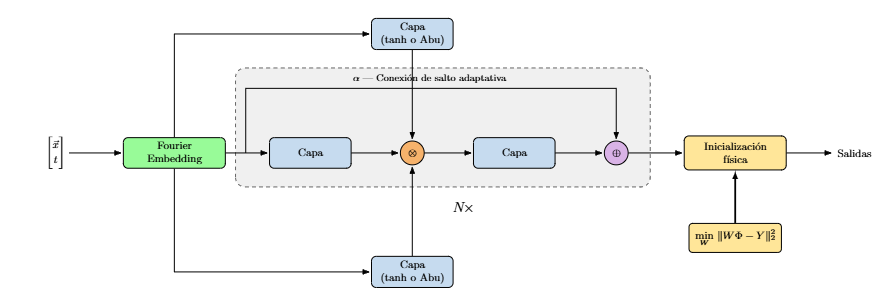
\includegraphics[width=\linewidth]{mabur_architecture.png}
  \caption[MABUR-PINN architecture]{MABUR-PINN architecture, based on PirateNet \cite{wang2024piratenets}: gates $U$ and $V$
  and the residual trunk with adaptive skip connections. Each dense block has three layers with $N$
  neurons. In Version~1 every neuron contains an Abu unit with $\{\sin,\cos,\tanh,\text{rational}\}$ and
  there is no Fourier embedding; in Version~2 the first layer of the trunk and of $U,V$ uses only $\tanh$,
  and there is a Fourier embedding.}
  \label{fig:mabur}
\end{figure}

\begin{table}[htbp]
  \centering
  \caption{The two versions of MABUR-PINN.}
  \label{tab:mabur-versions}
  \small
  \begin{tabularx}{\linewidth}{@{}lXX@{}}
    \toprule
    Property & Version 1 & Version 2 \\
    \midrule
    Implementation        & Monolithic class & Modular, four classes (modified MLP of Wang et al.~\cite{wang2021gradient}) \\
    Fourier embedding     & No & Yes, 256 random features, $\sigma=1.0$ \\
    Adaptive activation layer & AbuLayer: softmax blend of $\sin,\cos,\tanh$, rational & AbuLayer\_UV: same blend, with $U/V$ gating in a separate layer \\
    Encoders $U$ / $V$    & Adaptive layer (trainable activations) & Dense + $\tanh$ (fixed activation) \\
    Initial projection    & Adaptive layer with SIREN initialization & Dense + $\tanh$ with Glorot initialization \\
    Skip connections      & Every 3 layers & Every 2 layers \\
    $\omega_0$ (SIREN)    & 15.0 & 15.0 \\
    \bottomrule
  \end{tabularx}
\end{table}

\paragraph{Theoretical intuition.}
The Sobolev--Barron theorem (Theorem~\ref{thm:barron}) only sees the activation through the constant
$C_1=\max_{m\le\ell}\norm{\sigma^{(m)}}_{L^\infty}$. This motivates the following assumption on the family
of adaptive activations.

\begin{supuesto}{Adaptive softmax activations.}\label{asm:softmax}
Let $\Omega\subset\mathbb{R}^d$ be a bounded open domain, $\mu$ a probability measure on $\Omega$, and $\ell\in\mathbb{N}$
the maximum order of the differential operator of the PDE. Consider the family of adaptive softmax
activations
\[
  \mathcal{S}_{\mathrm{softmax}}:=\Big\{\sigma_{\mathrm{ad}}(x)=\sum_{i=1}^{N}\frac{e^{\alpha_i}}{\sum_{j=1}^{N}e^{\alpha_j}}\,\sigma_i(\beta_ix)\ \Big|\
  \bm\alpha\in\mathbb{R}^{N},\ \beta_i\in[\beta_{\min},\beta_{\max}]\subset(0,\infty)\Big\}.
\]
We assume that $\mathcal{S}_{\mathrm{softmax}}$ satisfies:
\begin{enumerate}
  \item \textbf{Uniform $C_1$ regularity:}
    $\displaystyle\sup_{\sigma_{\mathrm{ad}}\in\mathcal{S}_{\mathrm{softmax}}}\max_{m\le\ell}\norm{\sigma^{(m)}_{\mathrm{ad}}}_{L^\infty(\mathbb{R})}\le C_{1,\mathrm{ad}}<\infty.$
  \item \textbf{Sobolev--Barron approximation:} the conclusion of Theorem~\ref{thm:barron} holds for shallow
    networks whose activation is any fixed $\sigma_{\mathrm{ad}}\in\mathcal{S}_{\mathrm{softmax}}$, with
    $C_1$ replaced by $C_{1,\mathrm{ad}}$.\verificar{this condition is stated without content in the
    presentation; its validity must be checked or proved}
\end{enumerate}
\end{supuesto}

The first condition can actually be verified. Since the softmax weights $w_i$ are positive and sum to one,
by the chain rule
\begin{equation}
  \abs{\sigma^{(m)}_{\mathrm{ad}}(x)}=\Big|\sum_{i=1}^{N}w_i\beta_i^{m}\sigma_i^{(m)}(\beta_ix)\Big|
  \le\max_{1\le i\le N}\beta_{\max}^{m}\norm{\sigma_i^{(m)}}_{L^\infty(\mathbb{R})},
  \label{eq:abu-bound}
\end{equation}
so $C_{1,\mathrm{ad}}\le\max_{m\le\ell}\max_i\beta_{\max}^{m}\norm{\sigma_i^{(m)}}_{L^\infty}$, a bound that is
\emph{uniform in} $\bm\alpha$: whatever blend the optimizer learns, it can never be worse than the worst
branch at the largest scale. Two intuitions follow. First, condition~1 holds for the branches
$\{\sin,\cos,\tanh,1/(1+x^2)\}$ used for the Klein--Gordon equation (and for the Gaussian branch
$e^{-x^2}$), because they are bounded with bounded derivatives, but it fails for unbounded branches such as
Swish, Softplus or $e^{\beta x}-1$, which appear in some of the benchmark configurations
(Table~\ref{tab:benchmark-activations}). Second, the constant grows like $\beta_{\max}^{\ell}$: for the
Klein--Gordon equation ($\ell=2$) and the SIREN scale $\omega_0=15$, the factor is of order $225$. Large
scales give access to high frequencies, but they make the constant (and, by Theorem~\ref{thm:spectral-bias}, the
conditioning) worse. This is the same trade-off that $\sigma$ controls in a Fourier embedding, now learned
inside a bounded range. We stress that these are intuitions: the theorem is for shallow networks with a
single activation, while MABUR-PINN is a deep gated network whose neurons have different activations.

\paragraph{Activation functions.}
Table~\ref{tab:abu-branches} lists the candidate branches considered, with the analytical property that
justifies each of them in a PDE.

\begin{table}[htbp]
  \centering
  \caption{Candidate branches of the adaptive activation.}
  \label{tab:abu-branches}
  \small
  \begin{tabularx}{\linewidth}{@{}llX@{}}
    \toprule
    Function & Formulation $f(x)$ & Analytical property / justification in the PDE \\
    \midrule
    Sine & $\sin(\beta_ix)$ & Captures oscillatory dynamics and spatial/temporal harmonic modes. \\
    $\tanh$ & $\dfrac{e^{\beta_ix}-e^{-\beta_ix}}{e^{\beta_ix}+e^{-\beta_ix}}$ & Numerical stability; models smooth transition profiles. \\
    Swish / SiLU & $\dfrac{x}{1+e^{-\beta_ix}}$ & Good behavior of gradients in deep networks, without abrupt cancellations. \\
    Rational & $p(x)/q(x)$, e.g.\ $1/(1+(\beta_ix)^2)$ & Captures poles, asymptotes and boundary layers; high expressivity with few parameters. \\
    Exponential & $e^{\beta_ix}-1$ & Designed to capture boundary layers, strict dissipation and exponential decays. \\
    \bottomrule
  \end{tabularx}
\end{table}

\end{hyphenrules}
 % Physics-Informed Neural Networks - PINN
% !TEX root = 0000.tex
% Capítulo 3: Experimentation and Results
% Contenido tomado de main_2.tex (líneas 2623-3212) sin cambios de texto.

% El texto está en inglés: reglas de corte de palabra del inglés
\begin{hyphenrules}{english}

\chapter{Experimentation and Results}\label{ch:experiments}

This chapter evaluates the architectures of Chapter~\ref{ch:pinns} along two complementary lines. The first
one is a controlled case study, the linear homogeneous Klein--Gordon equation (Section~\ref{sec:klein-gordon}),
where the reference solution is exact in time and the number of frequencies of the initial condition can
be controlled; it contains a preliminary optimization experiment (Section~\ref{sec:exp-preliminary}), the
comparison of architectures (Section~\ref{sec:exp-architectures}) and a study of regularization and of the
Fourier scale (Section~\ref{sec:exp-regularization}). The second line is breadth: MABUR-PINN is evaluated on
twelve tasks of the PINNacle benchmark, which contain elliptic, parabolic and hyperbolic equations
(Section~\ref{sec:exp-benchmark}). Section~\ref{sec:exp-synthesis} relates the results with the theory of
Chapters~\ref{ch:pdes} and \ref{ch:pinns}.

% =====================================================================
\section{General Methodology}\label{sec:exp-methodology}
% =====================================================================

\paragraph{Metrics.}
For all experiments we report the relative $L^2$ error on a reference grid of
$N_{\mathrm{test}}$ points $(\mathbf{x}_j,t_j)$,
\begin{equation}
  \mathrm{L2RE}=\frac{\big(\sum_j\abs{u_\theta(\mathbf{x}_j,t_j)-u(\mathbf{x}_j,t_j)}^2\big)^{1/2}}{\big(\sum_j\abs{u(\mathbf{x}_j,t_j)}^2\big)^{1/2}},
  \label{eq:l2re}
\end{equation}
which is the discrete version of the total error $\mathcal{E}(\theta)$ of Section~\ref{sec:pinn-formulation};
the mean absolute error; the number of trainable parameters; and the final value of the (weighted)
loss, which is the training error $\mathcal{E}_T^2$. Reporting both the loss and the L2RE is important,
because Theorem~\ref{thm:error-decomp} says that they are different things.

\paragraph{Implementation.}
All networks were implemented and trained by us under the same conditions. We used mixed precision:
32-bit floating point only for the parameters of the network, and 64-bit floating point for the
collocation points, the optimization coefficients, the back-propagated gradients, etc. The code and the
results are available in the repositories
\url{https://github.com/Emmaquantum/HPINN} and \url{https://github.com/Emmaquantum/Optimization_PINN}.
\verificar{framework (PyTorch/JAX), hardware (GPU), training time and number of random seeds per
configuration}

% =====================================================================
\section{Reference Solution: Pseudo-Spectral Propagator}\label{sec:reference-solution}
% =====================================================================

\paragraph{Problem.}
We consider the one-dimensional Klein--Gordon equation \eqref{eq:kg} in natural units ($m=c=\hbar=1$):
\begin{equation}
  \begin{cases}
    \partial_{tt}\phi(x,t)-\partial_{xx}\phi(x,t)+m^2\phi(x,t)=0, & x\in\Omega=[-L/2,L/2],\ t\in[0,T],\\
    \phi(-L/2,t)=\phi(L/2,t), & t\in[0,T],\\
    \phi(x,0)=A\exp\Big(-\dfrac{x^2}{2\sigma^2}\Big)\displaystyle\sum_{k\in\mathcal{K}}\big(e^{ikx}+e^{-ikx}\big), & x\in\Omega,\\
    \partial_t\phi(x,0)=0, & x\in\Omega.
  \end{cases}
  \label{eq:kg-problem}
\end{equation}
The initial conditions represent a stationary particle, that is, a localized pulse with zero initial
velocity. The initial position is a Gaussian envelope modulated by a symmetric phase, which induces
velocity in $+k$ and $-k$. This initial condition can be manipulated consciously so that the network
needs to learn high and low frequencies at the same time, by introducing a set of wavenumbers
$\mathcal{K}=\{k_1,k_2,\dots,k_n\}$ with $k_1<k_2<\dots<k_n$. Because of the dispersion relation
Equation~\eqref{eq:kg-dispersion}, each wavenumber travels with a different group velocity: the pulse disperses
inside the light cone $\abs{x}\le t$. The boundary condition is periodic, as required by the
pseudo-spectral method; however, with the chosen parameters the wave does not reach the boundary during
the simulation. In Experiment~1 we use $\mathcal{K}=\{1,5,10\}$, $\sigma=1$, $L=80$ and $T=36$.
\verificar{value of the amplitude $A$; the presentation writes $\Omega=[-L,L]$ but the figures show
$x\in[-40,40]$}

\paragraph{Choice of parameters.}
The solution of Equation~\eqref{eq:kg-problem} models the field of a free particle released into an (almost)
infinite space. To achieve this, the space must be large enough to model an infinite space, $L\gg\sigma$,
and the simulation time must be short enough so that the wave does not hit the boundary.
\begin{enumerate}
  \item \textbf{Space:} $L\ge40\sigma$, enough times $\sigma$ so that the boundary is not reached.
  \item \textbf{Time:} since the group velocity is bounded by $c=1$ (Equation~\eqref{eq:kg-group-velocity}), the
    fastest front reaches the boundary at $t=L/2$. The thickness of the pulse is about $4\sigma$, so we
    take $T\approx L/2-4\sigma$; for $L=80$ and $\sigma=1$, $T=36$.
  \item \textbf{Grid:} in a classical explicit scheme we would need the CFL (Courant--Friedrichs--Lewy)
    condition $c\,\Delta t/\Delta x\le1$. Here the propagator is exact in time, so the scheme is
    unconditionally stable, and the time step only defines the temporal resolution of the stored
    solution. What matters is that the spatial grid resolves the largest wavenumber of the initial
    condition: with $N$ grid points, $\Delta x=L/N$ and we need $k_{\max}<\pi/\Delta x$. With $N=1000$ and
    $L=80$, $\pi/\Delta x\approx39>k_{\max}=10$.\verificar{whether $N=1000$ is the number of spatial points
    or of time steps}
\end{enumerate}

\paragraph{Propagator.}
The solution is exact in Fourier space, which means that, by means of a propagator
\cite{hochbruck2010}, the solution is computed without numerical errors beyond the truncation of the
Fourier series; all we have to do is to compute the propagator and iterate. With the change of variables
$v=\partial_t\phi$ and the operator $\mathcal{L}=m^2-\partial_{xx}$, the Klein--Gordon equation becomes
the first-order system
\begin{equation}
  \frac{\,d}{\,d t}\begin{pmatrix}\phi\\ v\end{pmatrix}
  =\underbrace{\begin{pmatrix}0 & 1\\ -\mathcal{L} & 0\end{pmatrix}}_{A}
  \begin{pmatrix}\phi\\ v\end{pmatrix},
  \qquad\mathbf{y}(t)=e^{At}\mathbf{y}(0),
  \label{eq:kg-first-order}
\end{equation}
with $\mathbf{y}=(\phi,\partial_t\phi)^{T}$. The propagator $e^{At}$ is responsible for the temporal
evolution of the field. Expanding it in Taylor series and separating the even and odd powers of $A$
(Appendix~\ref{app-sec:kg-propagator}), we obtain
\begin{equation}
  e^{At}=\begin{pmatrix}
    \cos\big(t\sqrt{\mathcal{L}}\big) & \dfrac{\sin(t\sqrt{\mathcal{L}})}{\sqrt{\mathcal{L}}}\\[2mm]
    -\sqrt{\mathcal{L}}\sin\big(t\sqrt{\mathcal{L}}\big) & \cos\big(t\sqrt{\mathcal{L}}\big)
  \end{pmatrix}.
  \label{eq:kg-propagator}
\end{equation}
To evaluate the
operator $\mathcal{L}$ numerically we take advantage of the periodic boundary condition: the Fourier
transform diagonalizes it, $\widehat{\mathcal{L}}=m^2-(ik)^2=m^2+k^2=\omega_k^2$, and the propagator becomes
a $2\times2$ rotation for each wavenumber:
\begin{equation}
  \begin{pmatrix}\hat\phi_k(t)\\ \hat{\dot\phi}_k(t)\end{pmatrix}
  =\begin{pmatrix}
    \cos(\omega_kt) & \dfrac{\sin(\omega_kt)}{\omega_k}\\[2mm]
    -\omega_k\sin(\omega_kt) & \cos(\omega_kt)
  \end{pmatrix}
  \begin{pmatrix}\hat\phi_k(0)\\ \hat{\dot\phi}_k(0)\end{pmatrix}.
  \label{eq:kg-propagator-fourier}
\end{equation}
This is exactly the discrete version of the exact solution \eqref{eq:kg-fourier-solution}. The algorithm
is Algorithm~\ref{alg:pseudospectral}.

\begin{algorithm}[htbp]
  \caption{Pseudo-spectral method for the Klein--Gordon equation.}
  \label{alg:pseudospectral}
  \begin{algorithmic}[1]
    \Require Physical parameters $m$, $L$, $T$, $N$; initial conditions $\phi(x,0)$, $\dot\phi(x,0)$.
    \State $\Delta x\gets L/N$, $\Delta t\gets T/N_t$ \Comment{precomputation of the frequency space}
    \State $k\gets 2\pi\cdot\texttt{fftfreq}(N,\Delta x)$; \quad $\omega_k\gets\sqrt{m^2+k^2}$
    \State $\hat\phi_k\gets\mathrm{FFT}(\phi(x,0))$; \quad $\hat{\dot\phi}_k\gets\mathrm{FFT}(\dot\phi(x,0))$ \Comment{initial transform}
    \State $C_k\gets\cos(\omega_k\Delta t)$; \quad $S_k\gets\sin(\omega_k\Delta t)$
    \State $t\gets0$
    \While{$t<T$} \Comment{time evolution, Equation~\eqref{eq:kg-propagator-fourier}}
      \State $\hat\phi^{\mathrm{new}}_k\gets C_k\hat\phi_k+\frac{1}{\omega_k}S_k\hat{\dot\phi}_k$
      \State $\hat{\dot\phi}^{\mathrm{new}}_k\gets-\omega_kS_k\hat\phi_k+C_k\hat{\dot\phi}_k$
      \State $\hat\phi_k\gets\hat\phi^{\mathrm{new}}_k$; \quad $\hat{\dot\phi}_k\gets\hat{\dot\phi}^{\mathrm{new}}_k$; \quad $t\gets t+\Delta t$
      \State store $\phi(x,t)\gets\operatorname{Re}\big(\mathrm{IFFT}(\hat\phi_k)\big)$ \Comment{recovery to real space}
    \EndWhile
    \State \Return history $\phi(x,t)$
  \end{algorithmic}
\end{algorithm}

Figure~\ref{fig:ps-evolution} shows the initial condition and the evolution of the field used in the
preliminary experiment. The field disperses inside a light cone, at the same velocity to the left and
to the right.

\begin{figure}[htbp]
  \centering
  \begin{subfigure}[b]{0.36\linewidth}
    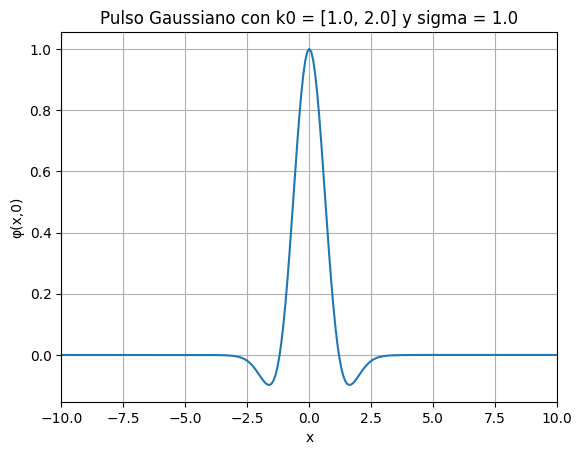
\includegraphics[width=\linewidth]{ic_gaussian.png}
    \caption{Initial condition (Gaussian pulse).}
  \end{subfigure}\hfill
  \begin{subfigure}[b]{0.62\linewidth}
    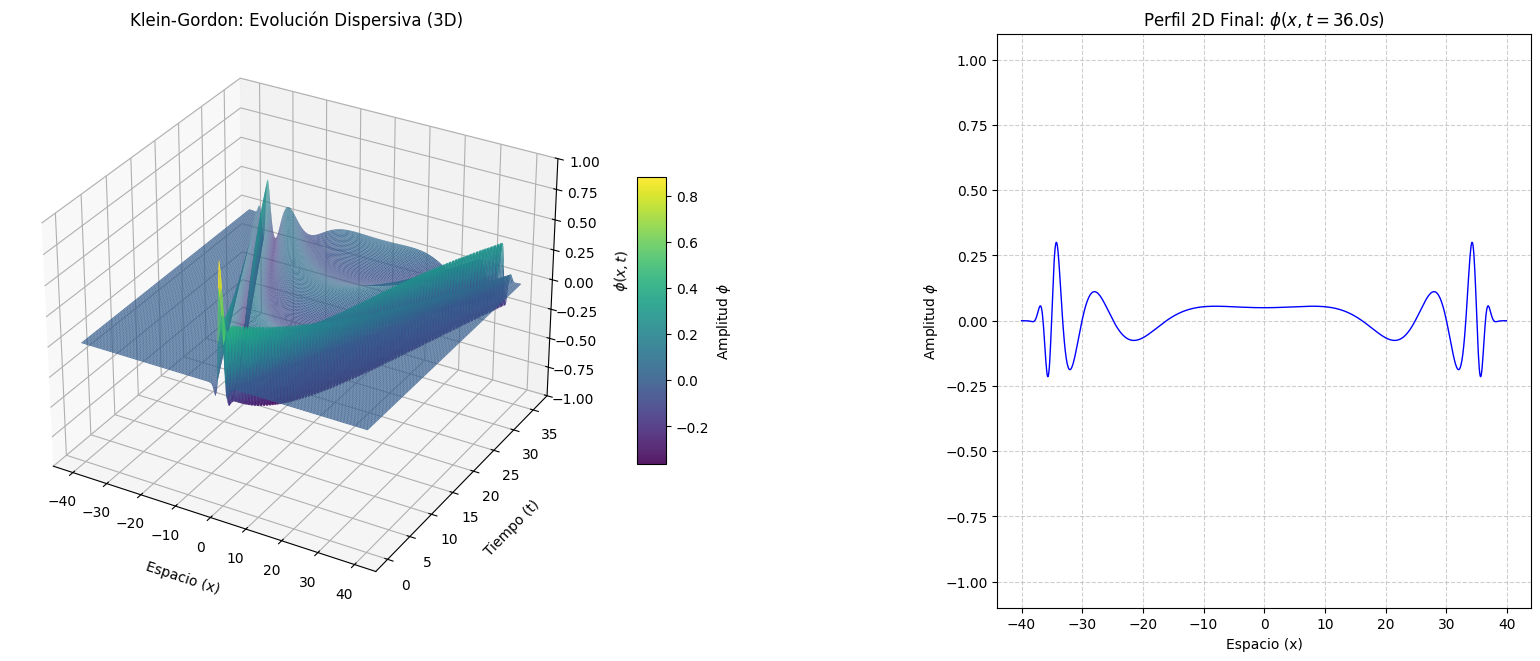
\includegraphics[width=\linewidth]{ps_evolution.png}
    \caption{Evolution of the field and final profile.}
  \end{subfigure}
  \caption[Pseudo-spectral reference solution of the preliminary experiment]{Pseudo-spectral reference solution of the preliminary experiment. (a) Initial condition,
  Gaussian with $\sigma=1$. (b) Evolution of the field during $36$ time units: the field disperses
  inside a light cone at the same velocity to the left and to the right, and the final profile shows
  the dispersion of the pulse once released in the (almost) infinite domain. A video of the evolution is
  available in the repository.}
  \label{fig:ps-evolution}
\end{figure}
\verificar{the text of the first report says $k_0=0.5$, but the title of panel (a) says $k_0=[1,2]$}

% =====================================================================
\section{Preliminary Experiment: ADAM + LRA and L-BFGS}\label{sec:exp-preliminary}
% =====================================================================

The first experiment asks a simple question: how well can a PINN with a periodic activation, trained with
the strategies of Section~\ref{sec:gradient-pathologies}, reproduce the dispersion of a static spin-0 particle?
We used a SIREN network ($\omega_0=30$) with $128$ neurons per hidden layer and $6$ hidden layers; this
architecture was obtained by experimentation until a good performance was reached. We used ADAM + LRA as a
first stage to characterize the minima within the set of achievable values: exponential decay of the
learning rate with $\eta_0=10^{-4}$ and rate $0.95$ every $1\,500$ iterations; the weights of the initial
and boundary losses were recomputed every $10$ iterations and updated with a moving average with
$\alpha=0.95$, starting from $(1,1,1)$. A random sampling algorithm generated new points
$(\mathbf{x}_i,t_i)$, $i\in\{f,ic,bc\}$, at each iteration \cite{wang2021gradient,liu2022}, starting from $128$
collocation points for each loss term; in this way, after $50\,000$ iterations the network was trained
with a total of $6.4$ million collocation points without saturating the memory.\verificar{the report
mentions both $50\,000$ and $100\,000$ ADAM iterations} After ADAM + LRA found a region where the
optimal value is, a variant of L-BFGS was used as final minimizer, with a stopping criterion of $5\,000$
iterations or a tolerance of machine epsilon; the weights and parameters of the first stage were loaded as
initialization, so that the second stage has some ``memory'' of the first one. The physical conditions
were the same as in the numerical simulation.

\paragraph{Results.}
The optimizer ADAM + LRA reduced the total loss to orders of $10^{-5}$ after the training, with a final
learning rate of $\approx3.27\times10^{-6}$ and final weights $(1.0,\,4.90,\,0.82)$, reaching stability at
a Pareto value (Figure~\ref{fig:prelim-loss}a). Although there seems to be convergence, ADAM is slow when
converging to minima, but fast approaching them when the gradients are balanced; since they are not, LRA
was used, and the curve shows a lot of noise produced by the change of weights every $10$ epochs. The
SIREN method favors the boundary conditions, so the boundary loss can reach values close to $10^{-12}$; the
total loss remained in the hands of the physics (PDE) loss and the initial condition.

The second-order optimizer L-BFGS refined the solution, reaching a total loss of order $10^{-8}$
(Figure~\ref{fig:prelim-loss}b), with smooth curves, no numerical explosions, and convergence in fewer than
$500$ iterations, which indicates that the inherited weights were good enough for the optimizer to reach
an almost even convergence of all the loss terms. The PDE loss converged rapidly, indicating strong
learning of the Klein--Gordon equation, that is, the network learned not to violate the physical law.

\begin{figure}[htbp]
  \centering
  \begin{subfigure}[b]{0.49\linewidth}
    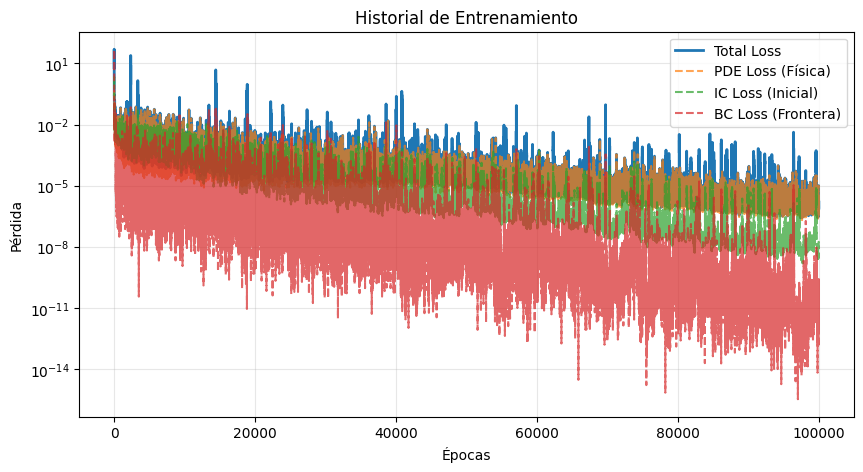
\includegraphics[width=\linewidth]{prelim_adam_loss.png}
    \caption{ADAM + LRA.}
  \end{subfigure}\hfill
  \begin{subfigure}[b]{0.49\linewidth}
    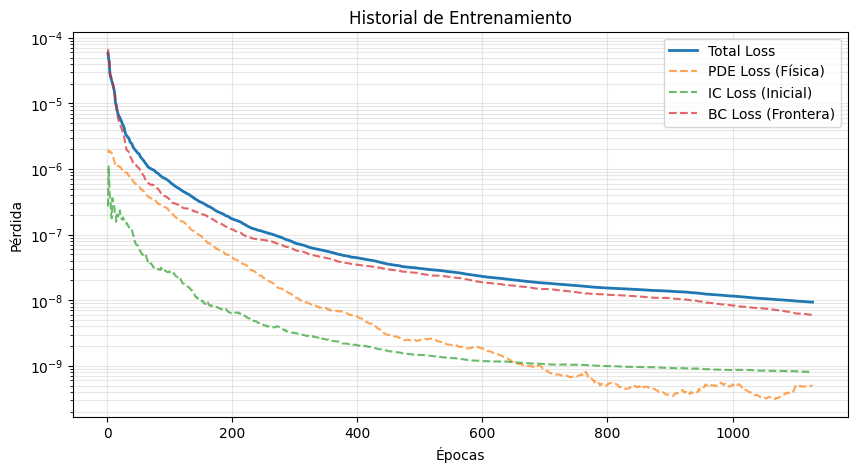
\includegraphics[width=\linewidth]{prelim_lbfgs_loss.png}
    \caption{L-BFGS.}
  \end{subfigure}
  \caption[Loss functions through the training epochs of the preliminary experiment]{Loss functions through the training epochs of the preliminary experiment. (a) ADAM + LRA:
  the noise comes from the update of the weights every $10$ epochs. (b) L-BFGS: smooth curves, without
  numerical explosions.}
  \label{fig:prelim-loss}
\end{figure}

Although the network learned the initial condition (Gaussian pulse) very well
(Figure~\ref{fig:prelim-validation}a), the validation against the numerical simulation shows conflicts: the
relative $L^2$ error is $9.53\%$ (Figure~\ref{fig:prelim-validation}b). The PINN generates the cone of the group
velocity of the fastest waves (inside the light cone), but it is still inconsistent in amplitude. We
interpret this result as an apparent Pareto value \cite{rohrhofer2023}: a training loss of order
$10^{-8}$ together with an error of almost $10\%$. In the language of Theorem~\ref{thm:error-decomp}, the training
error is small, but the generalization gap and the approximation error are not; this observation motivated
the comparison of architectures of the next section.

\begin{figure}[htbp]
  \centering
  \begin{subfigure}[b]{0.34\linewidth}
    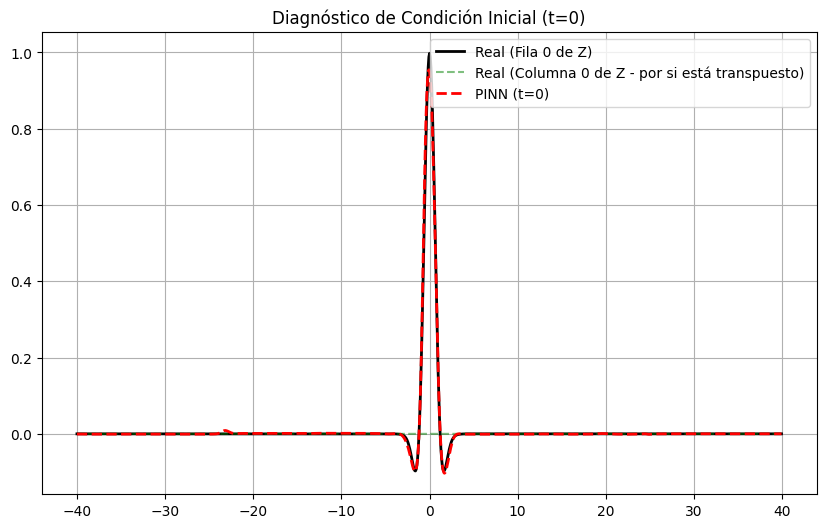
\includegraphics[width=\linewidth]{prelim_ic_diagnostic.png}
    \caption{Initial condition ($t=0$).}
  \end{subfigure}\hfill
  \begin{subfigure}[b]{0.64\linewidth}
    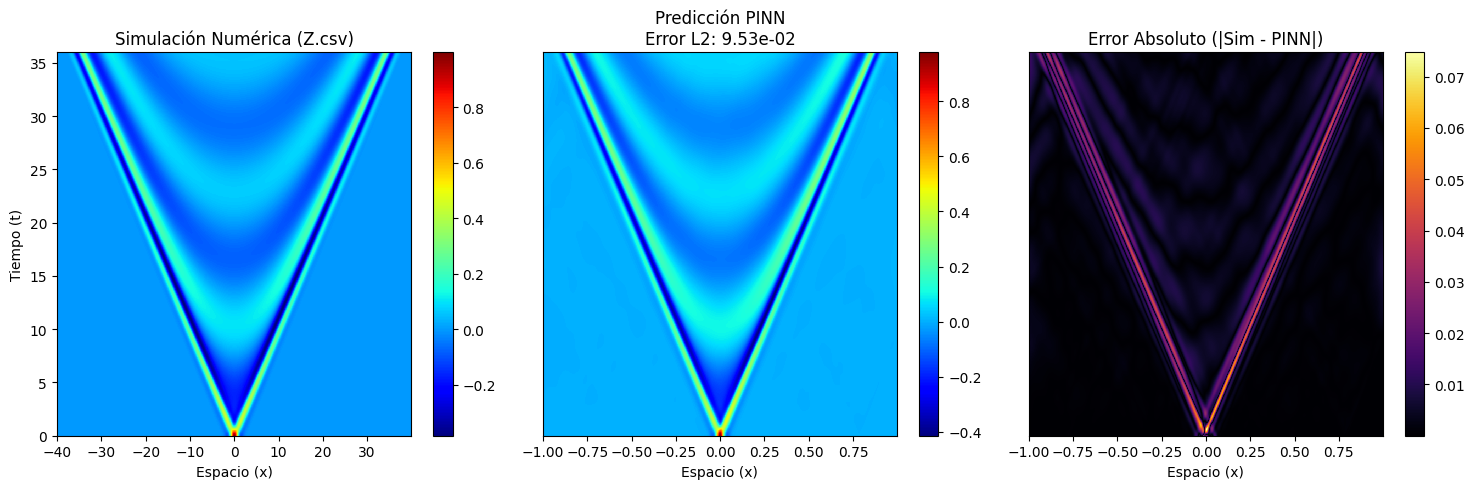
\includegraphics[width=\linewidth]{prelim_comparison.png}
    \caption{Simulation, PINN prediction and absolute error.}
  \end{subfigure}
  \caption[Validation of the preliminary experiment]{Validation of the preliminary experiment. (a) The network fits the static behavior at
  $t=0$ very well. (b) The PINN reproduces the light cone, but the amplitude inside the cone is still
  inconsistent (L2RE $=9.53\%$).}
  \label{fig:prelim-validation}
\end{figure}

% =====================================================================
\section{Experiment 1: Comparison of Architectures}\label{sec:exp-architectures}
% =====================================================================

\paragraph{Methodology.}
We replicated each of the architectures of Section~\ref{sec:architectures} and implemented them on the
Klein--Gordon problem \eqref{eq:kg-problem} with $\mathcal{K}=\{1,5,10\}$, to analyze their behavior. All
the networks were trained with the same strategies: input scaling (Equation~\eqref{eq:normalization}), learning rate
annealing (Section~\ref{subsec:lra}), causal training (Equation~\eqref{eq:causal}), focused stochastic sampling, exponential
decay of the learning rate and mixed precision. The shared configuration is given in
Table~\ref{tab:exp1-config}, and the specific settings of each architecture in Table~\ref{tab:exp1-architectures}.

\begin{table}[htbp]
  \centering
  \caption{Shared training configuration of Experiment~1.}
  \label{tab:exp1-config}
  \small
  \begin{tabular}{@{}ll@{}}
    \toprule
    Component & Configuration \\
    \midrule
    Optimizer & ADAM \cite{kingma2015} \\
    Loss weighting & LRA \cite{wang2021gradient}, $\alpha=0.9$ \\
    Temporal strategy & Causal training \cite{wang2024causality} \\
    Training epochs & $100\,000$ \\
    Learning rate & $10^{-3}$ initial, exponential decay $0.9$ every $2\,000$ epochs \\
    Physics collocation points ($N_f$) & $12\,000$ (80\% inside the light cone) \\
    Initial condition points ($N_{ic}$) & $N_f/2=6\,000$ \\
    Boundary points ($N_{bc}$) & $N_f/4=3\,000$ \\
    Normalization & min--max, $x\in[-1,1]$, $t\in[-1,1]$ \\
    Initial LRA weights & $(1.0,\,1.0,\,0.1)$ \\
    $\omega_0$ (architectures with $\sin$/$\cos$) & $15.0$ (SIREN, AbuPINN, MABUR-PINN) \\
    \bottomrule
  \end{tabular}
\end{table}
\verificar{the presentation reports $t\in[0,1]$ and initial LRA weights $(1,1,1,1)$; unify with the code}

\begin{table}[htbp]
  \centering
  \caption[Architectures of Experiment~1]{Architectures of Experiment~1 ($\epsilon$: causality parameter; chunks: number of temporal
  chunks of the causal loss).}
  \label{tab:exp1-architectures}
  \small
  \begin{tabularx}{\linewidth}{@{}lccccX@{}}
    \toprule
    Architecture & Depth & Width & $\epsilon$ & Chunks & Other \\
    \midrule
    Vanilla \cite{raissi2019} & 6 & 64 & 10 & 16 & $\tanh$ \\
    SIREN \cite{sitzmann2020} & 6 & 64 & 10 & 16 & SIREN activation \\
    MSF \cite{wang2021eigenvector} & 5 & 200 & 10 & 16 & Multiple embedding $\sigma$ \\
    M4 \cite{wang2021gradient} & 6 & 64 & 10 & 16 & Gated architecture + embedding \\
    Abu \cite{wang2023abu} & 6 & 64 & 100 & 16 & Blended activation \\
    MABUR (ours) & 6 (2 bl.) & 64 & 100 & 16 & M4 + Abu + adaptive residual \\
    \bottomrule
  \end{tabularx}
\end{table}

\paragraph{Results.}
Table~\ref{tab:exp1-results} summarizes the results, and Figure~\ref{fig:error-complexity} shows the relative error
against the complexity (number of parameters). MABUR-PINN V2 reaches the lowest error ($1.70\%$ relative
$L^2$) and the lowest final cost ($3.81\times10^{-7}$), followed by AbuPINN ($2.14\%$), which does it with
a moderate number of parameters ($42\,073$), and by M4-PINN ($4.41\%$). In contrast, the vanilla PINN shows
an almost total inability to solve the problem ($71\%$), while MSF-PINN, despite its high number of
parameters ($2.11\times10^{6}$), does not reduce the error significantly ($43.2\%$). MABUR-PINN V1, without
Fourier embedding, reaches $11.2\%$.

\begin{table}[htbp]
  \centering
  \caption{Comparative results of the architectures on the Klein--Gordon equation (Experiment~1).}
  \label{tab:exp1-results}
  \small
  \begin{tabular}{@{}lrrrr@{}}
    \toprule
    Architecture & Rel.\ $L^2$ error (\%) & Abs.\ error & Parameters & Final cost \\
    \midrule
    MABUR-PINN V2 & \textbf{1.70}  & \textbf{0.0006} & 149\,020   & $\mathbf{3.81\times10^{-7}}$ \\
    AbuPINN       & 2.14  & 0.0008 & 42\,073    & $4.60\times10^{-7}$ \\
    M4-PINN       & 4.41  & 0.0013 & 124\,033   & $2.21\times10^{-6}$ \\
    MABUR-PINN V1 & 11.20 & 0.0037 & 51\,177    & $7.25\times10^{-6}$ \\
    PINN-SIREN    & 21.20 & 0.0068 & 21\,057    & $5.85\times10^{-6}$ \\
    MSF-PINN      & 43.20 & 0.0142 & 2\,110\,049 & $9.99\times10^{-5}$ \\
    Vanilla PINN  & 71.00 & 0.0232 & 21\,057    & $6.72\times10^{-5}$ \\
    \bottomrule
  \end{tabular}
\end{table}
\verificar{single run or mean $\pm$ standard deviation over seeds}

\begin{figure}[htbp]
  \centering
  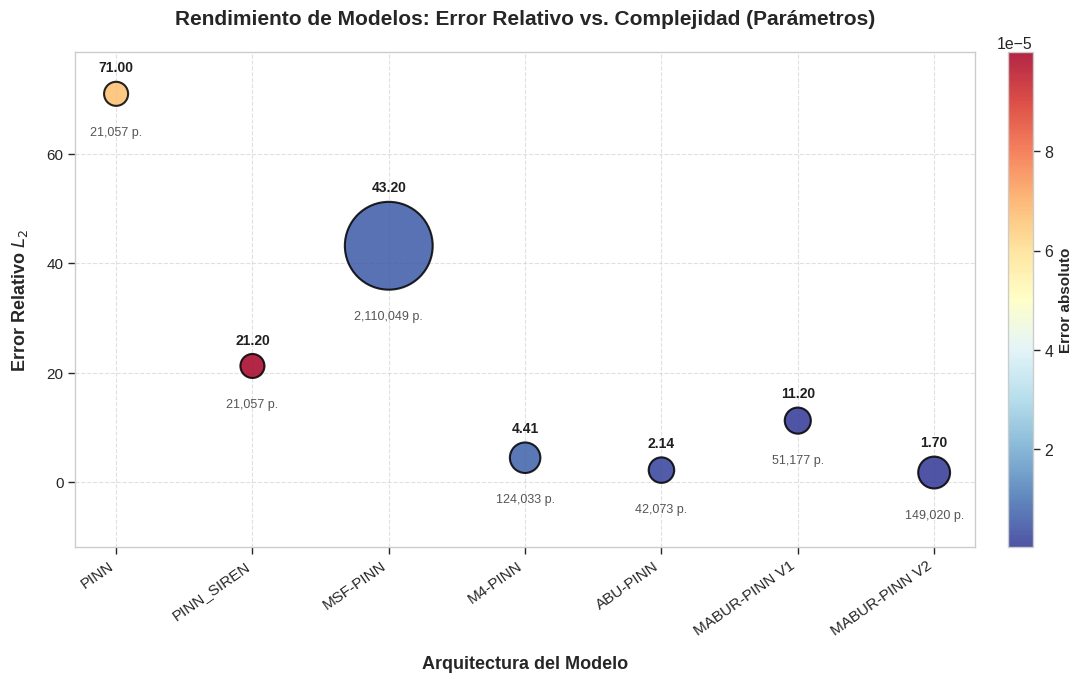
\includegraphics[width=0.85\linewidth]{error_vs_complexity.png}
  \caption[Relative $L^2$ error against complexity]{Relative $L^2$ error (\%) against complexity: the size of each marker is the number of
  parameters and the color is the absolute error.}
  \label{fig:error-complexity}
\end{figure}

Figure~\ref{fig:exp1-maps} compares the error maps of three representative networks; the error maps and loss
curves of all the architectures are in Appendix~\ref{app:figures}. The vanilla PINN has large errors distributed
over the whole cone. AbuPINN has a homogeneous error without pronounced peaks, except near the origin.
MABUR-PINN V2 concentrates its (small) error along the two fronts of the light cone.

\begin{figure}[htbp]
  \centering
  \begin{subfigure}[b]{\linewidth}
    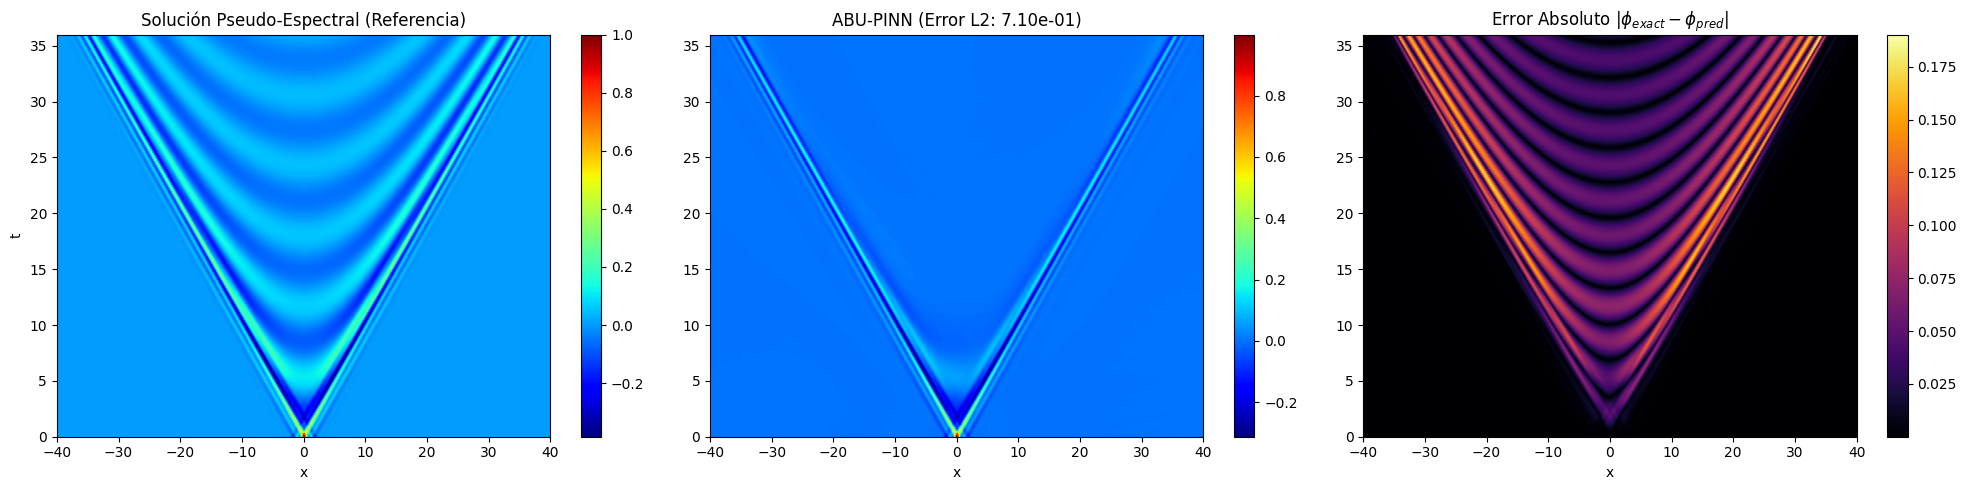
\includegraphics[width=\linewidth]{vanilla_error.png}
    \caption{Vanilla PINN (L2RE $71.0\%$).}
  \end{subfigure}
  \begin{subfigure}[b]{\linewidth}
    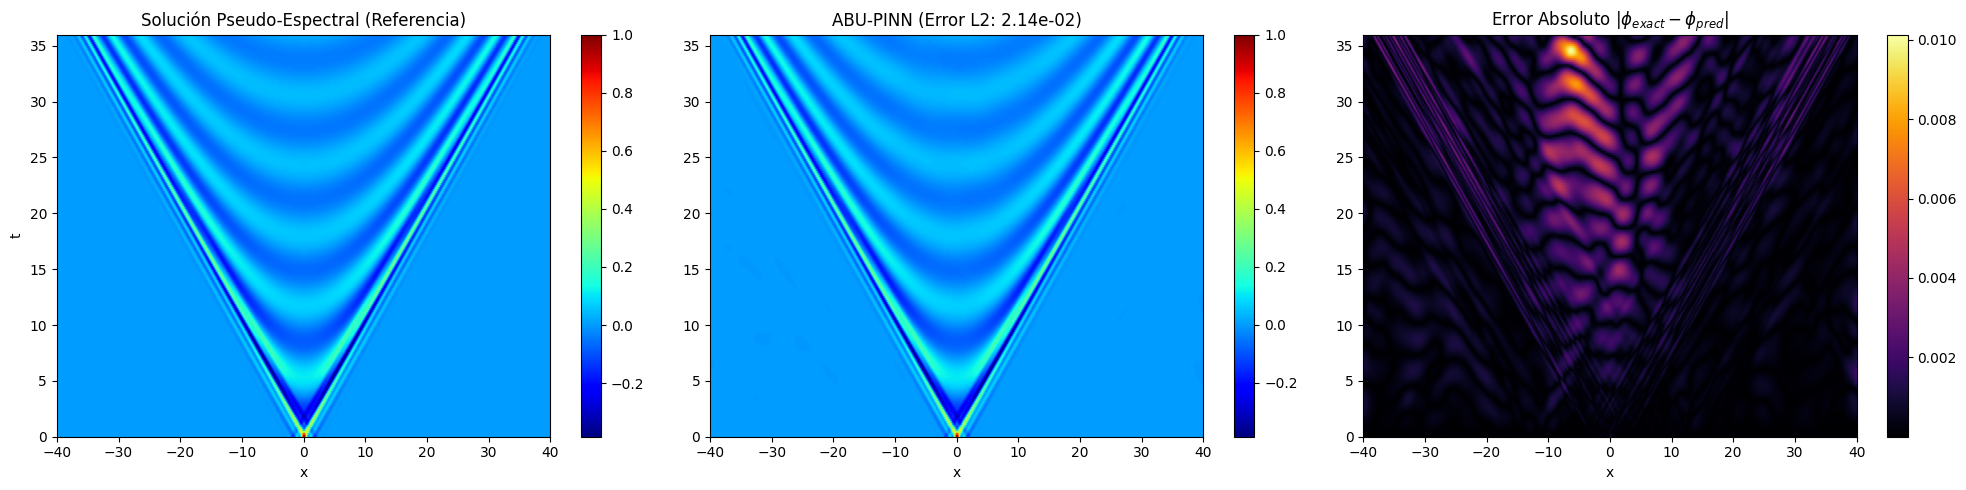
\includegraphics[width=\linewidth]{abu_error.png}
    \caption{AbuPINN (L2RE $2.14\%$).}
  \end{subfigure}
  \begin{subfigure}[b]{\linewidth}
    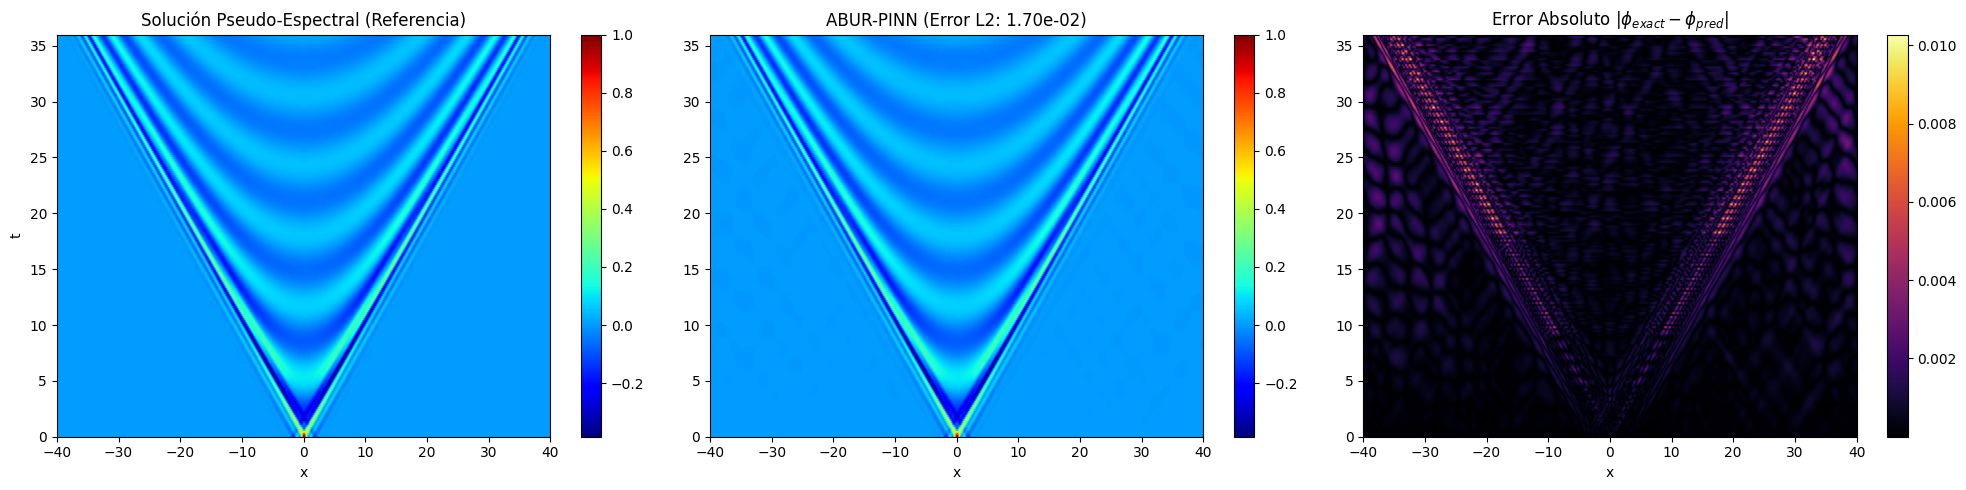
\includegraphics[width=\linewidth]{maburv2_error.png}
    \caption{MABUR-PINN V2 (L2RE $1.70\%$).}
  \end{subfigure}
  \caption[Error maps of three architectures on the Klein--Gordon equation]{Reference solution (left), prediction (center) and absolute error (right) for three
  architectures on the Klein--Gordon equation.}
  \label{fig:exp1-maps}
\end{figure}
\verificar{the panel titles of (a) say ``ABU-PINN'' and those of (c) ``ABUR-PINN''; regenerate the
figures with correct titles, in English}

\paragraph{Discussion.}
Several observations can be extracted.
\begin{enumerate}
  \item \textbf{A low value of the cost function does not guarantee a low relative error.} PINN-SIREN
    reaches a lower final cost than MABUR-PINN V1 ($5.85\times10^{-6}$ vs.\ $7.25\times10^{-6}$), and its
    boundary loss reaches $10^{-12}$, but its error is almost twice as large ($21.2\%$ vs.\ $11.2\%$).
    This is Theorem~\ref{thm:error-decomp} in practice: the training error is only one of the three terms.
  \item \textbf{Having many parameters does not solve, by itself, the optimization problems of hyperbolic
    PDEs if the architecture suffers from representability problems.} MSF-PINN has fifty times more
    parameters than AbuPINN and an error twenty times larger, with high variance in its training curves.
  \item \textbf{Adaptive activations are the decisive ingredient.} The three best networks (MABUR V2,
    AbuPINN and M4) all have either adaptive activations or multiplicative gates. AbuPINN is the most
    balanced architecture: low error with a moderate computational cost. Its ability to learn the optimal
    combination of activations (including sinusoids) is key for problems with periodic and rapidly
    varying components.
  \item \textbf{MABUR-PINN V2 improves the error, at a cost.} The improvement of V2 over AbuPINN is
    $0.44$ percentage points, with $3.5$ times more parameters. With a single run per configuration, this
    difference cannot yet be considered significant.
  \item \textbf{The remaining error lives on the fronts.} For MABUR-PINN (V1 and V2) the error is
    concentrated along the light cone, where the fastest components (the largest wavenumbers) travel. This
    agrees with the spectral bias (Equation~\eqref{eq:ntk-modes}) and with the conditioning of
    Theorem~\ref{thm:spectral-bias}: the highest frequencies are the last ones to be learned. V1 also shows
    difficulties representing the frequencies inside the cone.
  \item \textbf{The Fourier embedding still matters.} V1, without embedding, is clearly worse than V2,
    with an embedding of scale $\sigma=1$. Therefore, in its current form, MABUR-PINN reduces but does not
    eliminate the dependence on $\sigma$; Experiment~2 quantifies this dependence.
\end{enumerate}

% =====================================================================
\section{Experiment 2: Regularization and Fourier Scale}\label{sec:exp-regularization}
% =====================================================================

In this experiment, the model MABUR-PINN V2 was trained with and without regularization of the loss by the
derivatives of the residuals (Section~\ref{subsec:energy-estimate}), and with two values of the scale of the
Fourier embedding, to see the impact of each one (Table~\ref{tab:exp2}).

\begin{table}[htbp]
  \centering
  \caption[MABUR-PINN V2: regularization and Fourier scale]{MABUR-PINN V2 with and without derivative regularization, and with two Fourier scales
  (depth 6 with 2 blocks, width 64, $100\,000$ epochs).}
  \label{tab:exp2}
  \small
  \begin{tabular}{@{}lccr@{}}
    \toprule
    Model & Regularization & $\sigma$ & Rel.\ $L^2$ error (\%) \\
    \midrule
    MABUR-PINN V2 & No  & 1.0 & 1.70 \\
    MABUR-PINN V2 & Yes & 1.0 & 1.75 \\
    MABUR-PINN V2 & No  & 5.0 & 3.32 \\
    \bottomrule
  \end{tabular}
\end{table}
\verificar{which gradient terms were included in the regularized loss}

Two results stand out. First, the derivative regularization does not improve the error ($1.75\%$ vs.\
$1.70\%$). This is consistent with Theorem~\ref{thm:energy-estimate}: for periodic boundary conditions the
boundary terms cancel, and the only extra term required by the energy estimate is the gradient of the
initial position residual, which is already small because the initial condition is learned with high
accuracy. Second, increasing the Fourier scale from $\sigma=1$ to $\sigma=5$ doubles the error. Large
scales inject high frequencies from the beginning, which, according to Theorem~\ref{thm:spectral-bias} and the
bound \eqref{eq:abu-bound}, worsens the conditioning. The dependence on $\sigma$ is therefore reduced but
still present in MABUR-PINN V2.

\begin{figure}[htbp]
  \centering
  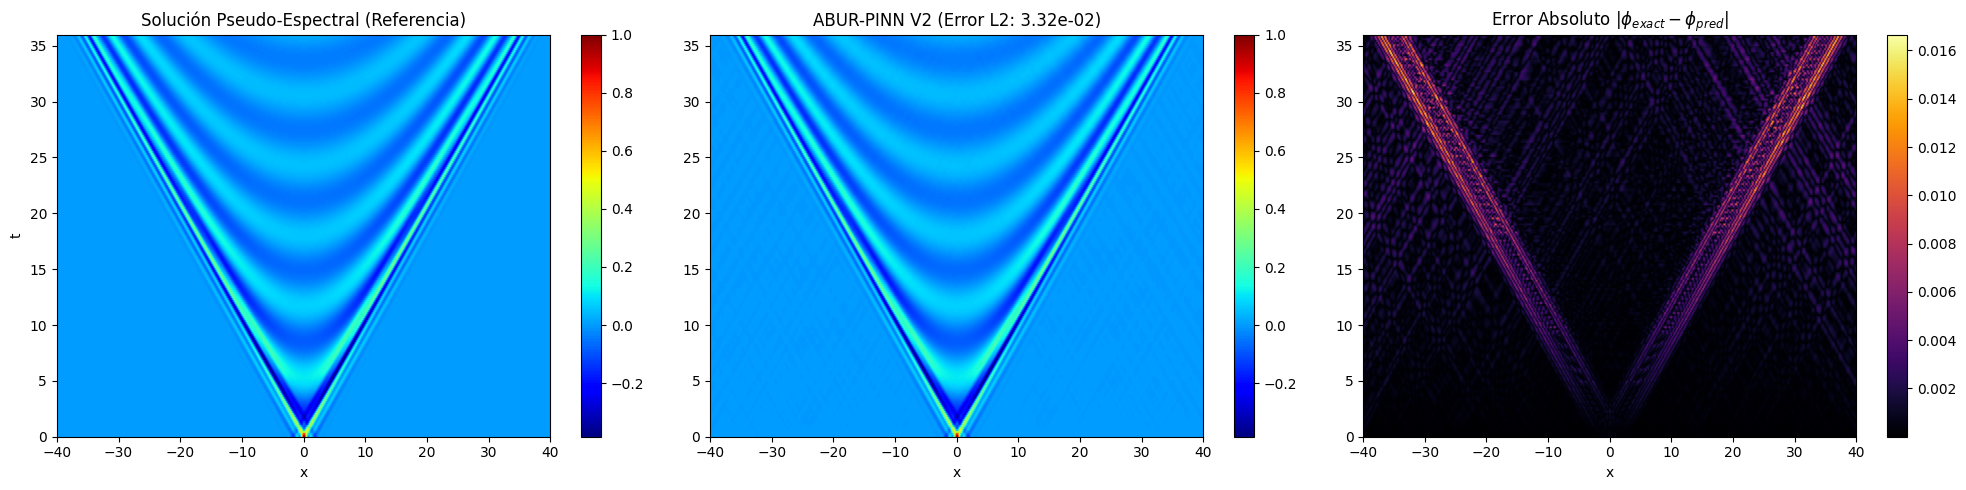
\includegraphics[width=\linewidth]{maburv2_sigma5_error.png}
  \caption[MABUR-PINN V2 with $\sigma=5$]{MABUR-PINN V2 with $\sigma=5$ (L2RE $3.32\%$): reference (left), prediction (center) and
  absolute error (right). The error is concentrated on the two fronts of the light cone.}
  \label{fig:exp2-sigma5}
\end{figure}
\verificar{in the first report this figure is under the heading ``V2 regularized''; check whether it
corresponds to $\sigma=5$ (its L2RE, $3.32\times10^{-2}$, matches $\sigma=5$)}

% =====================================================================
\section{Behavior of the Optimizer ADAM + LRA}\label{sec:exp-optimizer}
% =====================================================================

All the architectures were trained with ADAM and LRA to balance the terms of the composite loss. The final
losses (Table~\ref{tab:exp1-results}) show that MABUR-PINN V2 and AbuPINN reach the lowest values, followed by
M4-PINN and PINN-SIREN, while the vanilla PINN and MSF-PINN present higher losses (of order $10^{-5}$ and
$10^{-4}$), indicating difficulties to minimize simultaneously the PDE residual and the initial and
boundary conditions. The loss curves (Figure~\ref{fig:exp1-loss} and Appendix~\ref{app:figures}) show that:
\begin{itemize}
  \item ADAM + LRA reduces the total loss to orders between $10^{-7}$ and $10^{-5}$ after $10^{5}$
    epochs, but with noise due to the periodic readjustment of the weights $\lambda_i$;
  \item in AbuPINN, M4-PINN and MABUR-PINN the curves are more stable and the loss decreases rapidly,
    indicating a better balance of gradients; the total loss follows the physics loss, while the initial
    position loss decreases below $10^{-7}$;
  \item MSF-PINN shows high variance, probably because of its large number of parameters and the
    difficulty of training multi-scale embeddings.
\end{itemize}

\begin{figure}[htbp]
  \centering
  \begin{subfigure}[b]{0.49\linewidth}
    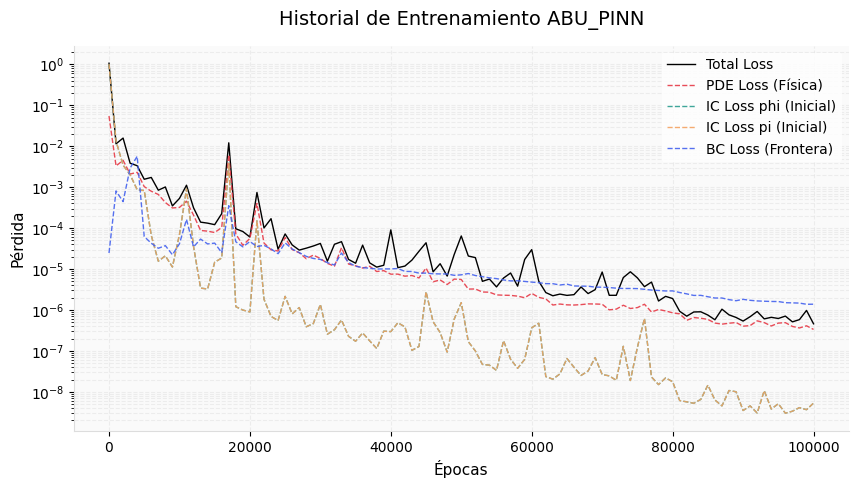
\includegraphics[width=\linewidth]{abu_loss.png}
    \caption{AbuPINN.}
  \end{subfigure}\hfill
  \begin{subfigure}[b]{0.49\linewidth}
    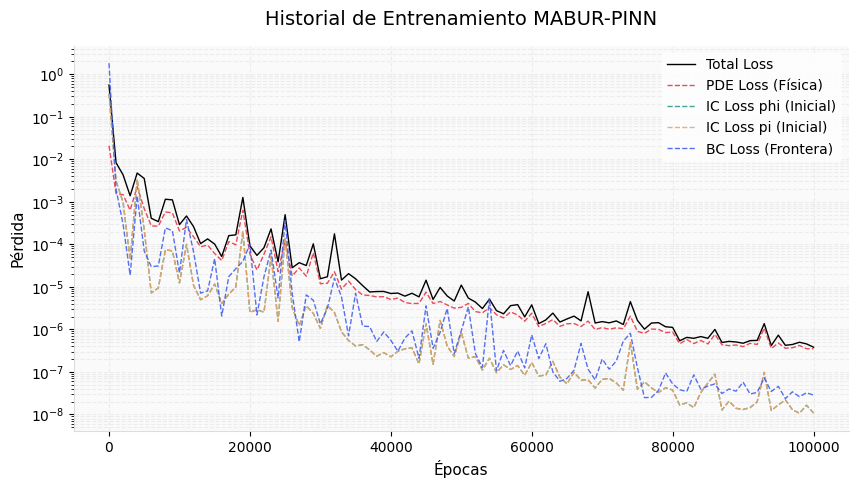
\includegraphics[width=\linewidth]{maburv2_loss.png}
    \caption{MABUR-PINN V2.}
  \end{subfigure}
  \caption{Training history (total, PDE, initial position, initial velocity and boundary losses).}
  \label{fig:exp1-loss}
\end{figure}

% =====================================================================
\section{Experiment 3: MABUR-PINN on the PINNacle Benchmark}\label{sec:exp-benchmark}
% =====================================================================

\paragraph{Methodology.}
To test whether the conclusions obtained for the Klein--Gordon equation extend to other classes of
PDEs, we adopted the experimental protocol of PINNacle \cite{hao2024pinnacle}. MABUR-PINN was evaluated
on a subset of $12$ tasks of the benchmark, covering elliptic (Poisson), parabolic (heat), hyperbolic
(wave) and nonlinear (Burgers, Navier--Stokes) equations in 1D and 2D (definitions in
Appendix~\ref{app:benchmark}). The results are compared against three representative methods of the benchmark:
LAAF, GAAF \cite{jagtap2020a,jagtap2020b} and FBPINN \cite{moseley2023}. Base configuration:
$5$ layers of $100$ neurons, $20\,000$ epochs, learning rate $10^{-3}$ (ADAM), $8\,192$ collocation points
and $2\,048$ boundary/initial points. LRA, causal training and Fourier embedding were \emph{not} used, in
order to adopt the experimental parameters of the benchmark. The branches of the softmax blend were chosen
for each family of PDEs (Table~\ref{tab:benchmark-activations}).

\begin{table}[htbp]
  \centering
  \caption[Branches of the softmax blend used for each PDE]{Branches of the softmax blend used for each PDE. $z=W\mathbf{x}+\mathbf{b}$ (dense branch, Glorot
  initialization); $z_s=\omega_0W_s\mathbf{x}$ (SIREN branch, $\omega_0=20$); output
  $=\sum_k\mathrm{softmax}(\bm\alpha)_k\sigma_k$.}
  \label{tab:benchmark-activations}
  \small
  \begin{tabularx}{\linewidth}{@{}llXc@{}}
    \toprule
    PDE & Variant & Branches & No. \\
    \midrule
    Burgers & 1d-C, 2d-C & $\sin(\beta_1z_s)$, $\tanh(\beta_2z)$, $1/(1+(\beta_3z)^2)$, $\ln(1+e^{\beta_4z})$, $e^{-(\beta_5z)^2}$ & 5 \\
    Poisson & 2d-C, 2d-CG, 2d-MS & $\ln(1+e^{\beta_1z})/\beta_1$, $z\,\sigma(\beta_2z)$ (Swish), $\tanh(\beta_3z)$, $1/(1+(\beta_4z)^2)$, $e^{-(\beta_5z)^2}$ & 5 \\
    Navier--Stokes & 2d-C & $\sin(\beta_1z_s)$, $\tanh(\beta_2z)$, $z\,\sigma(\beta_3z)$ (Swish), $e^{-(\beta_4z)^2}$ & 4 \\
    Wave & 1d-C & $\sin(z_s)$, $\cos(z_s)$, $\tanh(z)$, $1/(1+z^2)$ & 4 \\
    \bottomrule
  \end{tabularx}
\end{table}
\verificar{branches used for Heat, NS2d-CG, Wave2d-CG and Wave2d-MS}

\paragraph{Results.}
Table~\ref{tab:benchmark} shows the relative $L^2$ errors. MABUR-PINN obtains the best result in $8$ of the $12$
tasks: Burgers1d-C, Poisson2d-CG, Heat2d-MS, Heat2d-VC, NS2d-C, NS2d-CG, Wave1d-C and Wave2d-MS. LAAF is
the best in three tasks (Burgers2d-C, Poisson2d-MS, Heat2d-CG), FBPINN in Poisson2d-C and GAAF in
Wave2d-CG.

\begin{table}[htbp]
  \centering
  \caption[Relative $L^2$ error (L2RE) on the PINNacle benchmark]{Relative $L^2$ error (L2RE) on the PINNacle benchmark. In bold, the best result of each row.
  Data of LAAF, GAAF and FBPINN taken from Hao et al.~\cite[Table~3]{hao2024pinnacle}.}
  \label{tab:benchmark}
  \small
  \begin{tabular}{@{}llcccc@{}}
    \toprule
    PDE & Variant & LAAF & GAAF & FBPINN & MABUR-PINN \\
    \midrule
    \multirow{2}{*}{Burgers} & 1d-C & $1.43\times10^{-2}$ & $5.20\times10^{-2}$ & $2.32\times10^{-1}$ & $\mathbf{6.35\times10^{-3}}$ \\
                             & 2d-C & $\mathbf{2.77\times10^{-1}}$ & $2.95\times10^{-1}$ & -- & $4.67\times10^{-1}$ \\
    \midrule
    \multirow{3}{*}{Poisson} & 2d-C  & $7.68\times10^{-1}$ & $6.04\times10^{-1}$ & $\mathbf{4.49\times10^{-2}}$ & $6.03\times10^{-2}$ \\
                             & 2d-CG & $4.80\times10^{-1}$ & $8.71\times10^{-1}$ & $2.90\times10^{-2}$ & $\mathbf{2.98\times10^{-3}}$ \\
                             & 2d-MS & $\mathbf{5.93\times10^{-1}}$ & $9.31\times10^{-1}$ & $1.04$ & $1.32$ \\
    \midrule
    \multirow{3}{*}{Heat}    & 2d-CG & $\mathbf{2.39\times10^{-2}}$ & $4.61\times10^{-1}$ & $9.16\times10^{-2}$ & $3.71\times10^{-2}$ \\
                             & 2d-MS & $7.40\times10^{-2}$ & $9.85\times10^{-1}$ & $8.20\times10^{-2}$ & $\mathbf{1.87\times10^{-2}}$ \\
                             & 2d-VC & $6.42\times10^{-1}$ & $8.49\times10^{-1}$ & $9.52\times10^{-1}$ & $\mathbf{2.25\times10^{-1}}$ \\
    \midrule
    \multirow{2}{*}{Navier--Stokes} & 2d-C  & $3.60\times10^{-2}$ & $3.79\times10^{-2}$ & $8.45\times10^{-2}$ & $\mathbf{1.20\times10^{-2}}$ \\
                                    & 2d-CG & $8.24\times10^{-2}$ & $1.74\times10^{-1}$ & $8.27$ & $\mathbf{6.32\times10^{-2}}$ \\
    \midrule
    \multirow{3}{*}{Wave}    & 1d-C  & $4.54\times10^{-1}$ & $6.77\times10^{-1}$ & $5.91\times10^{-1}$ & $\mathbf{3.53\times10^{-1}}$ \\
                             & 2d-CG & $8.19\times10^{-1}$ & $\mathbf{7.94\times10^{-1}}$ & $1.06$ & $1.42$ \\
                             & 2d-MS & $1.06$ & $1.06$ & $1.03$ & $\mathbf{9.86\times10^{-1}}$ \\
    \bottomrule
  \end{tabular}
\end{table}
\verificar{whether the PINNacle values are means over several runs and how many runs were made for
MABUR-PINN}

\paragraph{Discussion by class.}
\begin{itemize}
  \item \textbf{Parabolic (heat).} MABUR-PINN is the best in the multi-scale and variable-coefficient
    problems, where the adaptive scales $\beta_i$ seem to help, and is second in the complex geometry
    (behind LAAF). Parabolic problems are, as expected from Table~\ref{tab:second-order}, the ones where the
    errors are smaller overall.
  \item \textbf{Elliptic (Poisson).} The results are mixed: the best result by one order of magnitude in
    the complex geometry (CG), second in the classic problem (C), and a failure (L2RE $>1$) in the
    multi-scale problem (MS), as for all the methods except LAAF.
  \item \textbf{Nonlinear (Burgers, Navier--Stokes).} MABUR-PINN is the best in three of the four tasks.
    Burgers2d-C, whose solution develops steep fronts, remains difficult.
  \item \textbf{Hyperbolic (wave).} This is the hardest class, as predicted in
    Section~\ref{sec:regularity-bridge}. MABUR-PINN is the best in Wave1d-C ($0.353$), but all the methods fail
    in the 2D tasks (L2RE between $0.79$ and $1.42$), and MABUR-PINN is the worst in Wave2d-CG (heterogeneous medium
    $c(\mathbf{x})$); the reason for this failure has not been analyzed yet. In Wave2d-MS the comparison is not informative, because, as shown
    in Section~\ref{sec:klein-gordon} and Appendix~\ref{app:benchmark}, its reference solution satisfies a Klein--Gordon
    equation with mass $2\pi^2$ instead of the stated wave equation; a network that minimizes the residual
    of the wave equation cannot approach that reference.
\end{itemize}

\paragraph{Threats to validity.}
The baselines are the published values of PINNacle and were not re-run by us; the branches of the
activation were chosen per family of PDEs, which is an additional degree of tuning that the baselines did
not have; and MABUR-PINN was run once per task. These three facts limit the strength of the comparison,
and they are addressed in the checklist of future work.

% =====================================================================
\section{Synthesis}\label{sec:exp-synthesis}
% =====================================================================

The experiments confirm, at least qualitatively, the three intuitions of Section~\ref{sec:regularity-bridge}.
First, smoothing helps the learner: the parabolic problems are the ones with the smallest errors, while the
hyperbolic ones (wave and Klein--Gordon) concentrate the failures, and inside the Klein--Gordon problem the
error of the best networks lives on the light-cone fronts, where the highest frequencies travel. Second, the
energy estimate of Theorem~\ref{thm:energy-estimate} explains why the derivative regularization did not help in a
periodic problem. Third, a small loss is not a small error: the preliminary experiment ($10^{-8}$ loss,
$9.5\%$ error) and PINN-SIREN show it clearly, as predicted by Theorem~\ref{thm:error-decomp}.

Regarding the proposed architecture, MABUR-PINN V2 obtained the lowest error on the Klein--Gordon equation and
the best result in $8$ of $12$ tasks of the benchmark. At the same time, the experiments show that the
Fourier embedding is still needed (V1 vs.\ V2) and that the scale $\sigma$ still matters
(Table~\ref{tab:exp2}); the adaptive activations reduce, but do not remove, this dependence. The bound
Equation~\eqref{eq:abu-bound} gives a theoretical reason for using bounded branches and a bounded range of scales,
which suggests replacing Swish, Softplus and exponential branches, and constraining $\beta_{\max}$, in
future versions.

\end{hyphenrules}
 % Experimentation and Results
% !TEX root = 0000.tex
% Capítulo 4: PINNs en un frame cuántico
% Contenido tomado de main_2.tex (líneas 3217-3220) sin cambios de texto.

\chapter{Redes Neuronales Informadas por la física en un frame cuántico}\label{ch:quantum}\chaptermark{PINNs en un frame cuántico}
\section{Computación Cuántica Variacional}
\section{Circuitos Cuánticos Parametrizados (PQC) como aproximadores de funciones}
\section{Integración Híbrida: PINNs y Algoritmos Cuánticos}
 % Redes Neuronales Informadas por la física en un frame cuántico
% !TEX root = 0000.tex
% Capítulo 5: Conclusiones y recomendaciones
% Contenido tomado de main_2.tex (líneas 3225-3230) sin cambios de texto.

\chapter{Conclusiones y recomendaciones}\label{ch:conclusions}
\section{Conclusiones}
% (Pega aquí tus conclusiones: deben responder a los objetivos)

\section{Recomendaciones}
% (Trabajo futuro: qué se podría hacer para continuar o fortalecer esta investigación)
 % Conclusiones y recomendaciones

%Inicio del apéndice o anexos
\begin{appendix}
% !TEX root = 0000.tex
% Anexo A
% Contenido tomado de main_2.tex (líneas 3248-3574) sin cambios de texto.

% El texto está en inglés: reglas de corte de palabra del inglés
\begin{hyphenrules}{english}

\chapter{Anexo: Derivations of the Classical Representation Formulas}\chaptermark{Classical Derivations}\label{app:classical}

This appendix contains the complete derivations of the formulas of Section~\ref{sec:linear-pdes}, and of
the propagator used for the reference solution of Chapter~\ref{ch:experiments}. They follow
Evans~\cite{evans2010}; the equation numbers of the main text are cited where the result is used.

% ---------------------------------------------------------------------
\section{Transport Equation}\label{app-sec:transport}

The geometry of a function $u:\mathbb{R}^n\times[0,\infty)\to\mathbb{R}$ that satisfies $Lu=0$, for the transport
operator $L=\partial_t+\mathbf{b}\cdot\nabla$, is represented by the hypersurface $S\subset\mathbb{R}^{n+2}$ given by
\begin{equation}
  S=\{(\mathbf{x},t,z)\in\mathbb{R}^n\times[0,\infty)\times\mathbb{R} \mid \Phi(\mathbf{x},t,z)=u(\mathbf{x},t)-z=0\},
  \label{eq:transport-graph}
\end{equation}
where $S$ is simply the graph of the solution $u$. Transport inherently involves velocity and spatial
displacement; with the constant space--time vector field $\mathbf{V}=(\mathbf{b},1)^{T}\in\mathbb{R}^{n+1}$ we arrive at
the homogeneous transport equation $\partial_t u(\mathbf{x},t)+\mathbf{b}\cdot\nabla u(\mathbf{x},t)=0$.

\paragraph{Homogeneous case.}
For the problem \eqref{eq:transport-hom}, the matrix form of the system is
\begin{equation}
  \begin{pmatrix}\nabla u(\mathbf{x},t)\\ \partial_t u(\mathbf{x},t)\end{pmatrix}\cdot
  \begin{pmatrix}\mathbf{b}\\ 1\end{pmatrix}=0
  \iff D_{\mathbf{V}}u=\nabla_{\mathbf{x},t}u\cdot\mathbf{V}=0,
  \label{eq:transport-matrix}
\end{equation}
which establishes that the directional derivative of $u$ in the direction of the vector $\mathbf{V}$ is
identically zero throughout the space--time domain. This means that the velocity vector is perpendicular
to the gradient and tangent to the level sets of $u$. In other words, if one moves in the direction of
$\mathbf{V}$, the value of $u$ remains constant along the characteristic trajectory. The solution to
$D_{\mathbf{V}}u=0$ is $u(\mathbf{x},t)=g(\mathbf{x}-t\mathbf{b})$.

\paragraph{Non-homogeneous case.}
For the problem \eqref{eq:transport-nonhom} we apply the same approach as in the homogeneous case.
Consider the smooth function
$u:\mathbb{R}^n\times[0,\infty)\to\mathbb{R}$; the graph of the solution is again a hypersurface, now in the
$(n+2)$-dimensional space of triples $(\mathbf{x},t,z)$. At any point $(\mathbf{x},t,z)\in S$, the normal vector to
the tangent plane of the surface $S$ is given by the gradient of $\Phi$,
\begin{equation}
  D\Phi(\mathbf{x},t,z)=\big(\nabla u(\mathbf{x},t),\ \partial_t u(\mathbf{x},t),\ -1\big)^{T}.
  \label{eq:transport-normal}
\end{equation}
Thus, the PDE can be interpreted as a tangency condition. Inspired by the same idea as in the
homogeneous case, we define $z(s)=u(\mathbf{x}+s\mathbf{b},t+s)$ for $s\in[-t,0]$. Calculating the derivative yields
\begin{equation}
  \frac{\,d z}{\,d s}=\partial_t u(\mathbf{x}+s\mathbf{b},t+s)+\mathbf{b}\cdot\nabla u(\mathbf{x}+s\mathbf{b},t+s)=f(\mathbf{x}+s\mathbf{b},t+s),
  \label{eq:transport-dz}
\end{equation}
and integrating from $-t$ to $0$ gives
\begin{equation}
  z(0)-z(-t)=\int_{-t}^{0}\frac{\,d z}{\,d s}\,d s=\int_{-t}^{0}f(\mathbf{x}+s\mathbf{b},t+s)\,d s.
  \label{eq:transport-int}
\end{equation}
Given that $z(0)=u(\mathbf{x},t)$ and $z(-t)=u(\mathbf{x}-t\mathbf{b},0)=g(\mathbf{x}-t\mathbf{b})$, and using the change of variables
$\tau=t+s$, we obtain the expression
\begin{equation}
  u(\mathbf{x},t)=g(\mathbf{x}-t\mathbf{b})+\int_{0}^{t}f\big(\mathbf{x}+(\tau-t)\mathbf{b},\tau\big)\,d\tau.
  \label{eq:app-transport-duhamel}
\end{equation}
Through Duhamel's principle, this result means that the solution is the sum of the transported initial
value $g(\mathbf{x}-t\mathbf{b})$ and the values accumulated from the source $f$, generated in the past times $\tau$
along the same characteristic curve.

% ---------------------------------------------------------------------
\section{Laplace's Equation}\label{app-sec:laplace}

\paragraph{Green's representation formula.}
To integrate the boundary information of the problem \eqref{eq:laplace-dirichlet}, we employ a vector
field that contains
it; following Evans~\cite{evans2010}, we combine the harmonic function $u$ and the fundamental solution
$\Phi$ in the flux $\mathbf{F}=u\nabla\Phi-\Phi\nabla u$. By the divergence theorem (Green's second identity),
\begin{align}
  \int_\Omega\operatorname{div}(\mathbf{F})\,d\mathbf{y}
    &=\int_\Omega\big(u(\mathbf{y})\Delta\Phi(\mathbf{x}-\mathbf{y})-\Phi(\mathbf{x}-\mathbf{y})\Delta u(\mathbf{y})\big)\,d\mathbf{y} \label{eq:green2-a}\\
    &=\int_{\partial\Omega}\Big(u(\mathbf{y})\frac{\partial\Phi}{\partial\mathbf{n}}(\mathbf{x}-\mathbf{y})
      -\Phi(\mathbf{x}-\mathbf{y})\frac{\partial u}{\partial\mathbf{n}}(\mathbf{y})\Big)\,d S(\mathbf{y}), \label{eq:green2-b}
\end{align}
where $\partial f/\partial\mathbf{n}=\nabla f\cdot\mathbf{n}$ for $f\in\{u,\Phi\}$ and $\mathbf{n}$ is the outward normal vector
at $\partial\Omega$. On the right side of the first equation, $-\Delta\Phi(\mathbf{x}-\mathbf{y})=\delta(\mathbf{x}-\mathbf{y})$ at the
singular point and zero elsewhere, and $\Delta u(\mathbf{y})=0$ by definition; thus, only the singular point
survives and the integral equals $-u(\mathbf{x})$. On the boundary, $u(\mathbf{y})=g(\mathbf{y})$. Thus,
\begin{equation}
  u(\mathbf{x})=\int_{\partial\Omega}\Big(\Phi(\mathbf{x}-\mathbf{y})\frac{\partial u}{\partial\mathbf{n}}(\mathbf{y})
    -g(\mathbf{y})\frac{\partial\Phi}{\partial\mathbf{n}}(\mathbf{x}-\mathbf{y})\Big)\,d S(\mathbf{y}).
  \label{eq:laplace-rep}
\end{equation}

However, $\partial u/\partial\mathbf{n}$ is unknown on the boundary. To complement the previous idea and
eliminate the unknown term by the Green method, it is necessary to build an auxiliary (corrector)
function $\phi^{\mathbf{x}}\in C^2(\Omega)\cap C(\bar\Omega)$ that is harmonic in $\Omega$ and matches the
fundamental solution on the boundary, $\phi^{\mathbf{x}}(\mathbf{y})=\Phi(\mathbf{y}-\mathbf{x})$ for $\mathbf{y}\in\partial\Omega$. Applying
the same identity to the flux $\mathbf{F}=u\nabla\phi^{\mathbf{x}}-\phi^{\mathbf{x}}\nabla u$, where now both functions are
harmonic, we obtain
\begin{equation}
  0=\int_{\partial\Omega}\Big(g(\mathbf{y})\frac{\partial\phi^{\mathbf{x}}}{\partial\mathbf{n}}(\mathbf{y})
    -\Phi(\mathbf{x}-\mathbf{y})\frac{\partial u}{\partial\mathbf{n}}(\mathbf{y})\Big)\,d S(\mathbf{y}).
  \label{eq:laplace-corrector}
\end{equation}
By the superposition of Equations~\eqref{eq:laplace-rep} and \eqref{eq:laplace-corrector}, the unknown normal derivative
cancels and we finally find the solution $u$ through Green's function
$G(\mathbf{x},\mathbf{y})=\Phi(\mathbf{y}-\mathbf{x})-\phi^{\mathbf{x}}(\mathbf{y})$:
\begin{equation}
  u(\mathbf{x})=-\int_{\partial\Omega}g(\mathbf{y})\frac{\partial G}{\partial\mathbf{n}}(\mathbf{x},\mathbf{y})\,d S(\mathbf{y}),
  \label{eq:app-laplace-green}
\end{equation}
where $\partial G/\partial\mathbf{n}=\nabla_{\mathbf{y}}G\cdot\mathbf{n}$. Finally, we have an analytical solution through an
auxiliary function that imposes the cancellation on the boundary:
\begin{equation}
  \begin{cases}
    -\Delta_{\mathbf{y}}G(\mathbf{x},\mathbf{y})=\delta(\mathbf{x}-\mathbf{y}) & \text{in } \mathbf{y}\in\Omega,\\
    G(\mathbf{x},\mathbf{y})=0 & \text{on } \mathbf{y}\in\partial\Omega.
  \end{cases}
  \label{eq:app-green-function}
\end{equation}

\paragraph{Mean-value property (heuristic derivation).}
Consider a ball $B(\mathbf{x},r)\subset\Omega$ centered at a point $\mathbf{x}$ inside the domain. Applying
Equation~\eqref{eq:app-laplace-green} to the ball itself (homogeneous case),
\begin{equation}
  u(\mathbf{x})=-\int_{\partial B(\mathbf{x},r)}u(\mathbf{y})\frac{\partial G}{\partial\mathbf{n}}(\mathbf{x},\mathbf{y})\,d S(\mathbf{y}).
  \label{eq:mvp-1}
\end{equation}
Evaluating the $\partial G/\partial\mathbf{n}$ term on the sphere $\partial B(\mathbf{x},r)$ is easy for this geometry:
since $\Phi(\mathbf{y}-\mathbf{x})$ only depends on $r=\abs{\mathbf{x}-\mathbf{y}}$, it is constant on $\partial B(\mathbf{x},r)$, and the
corrector is simply the constant $\phi^{\mathbf{x}}\equiv\Phi(r)$, whose gradient vanishes. The derivative with
respect to the normal vector $\mathbf{n}$ is then
\begin{align}
  \frac{\partial G}{\partial\mathbf{n}}(\mathbf{x},\mathbf{y})
    &=\big(\nabla_r\Phi(r)-\nabla_r\phi^{\mathbf{x}}\big)\cdot\mathbf{n}=\nabla_r\Phi(r)\cdot\mathbf{n} \label{eq:mvp-2}\\
    &=\begin{cases}
        -\dfrac{1}{2\pi r} & (n=2),\\[2mm]
        -\dfrac{1}{n\alpha(n)}\dfrac{1}{r^{n-1}} & (n\ge3);
      \end{cases} \label{eq:mvp-3}
\end{align}
in both cases the denominator is the surface area $\abs{\partial B(\mathbf{x},r)}=n\alpha(n)r^{n-1}$, so
\begin{equation}
  u(\mathbf{x})=\frac{1}{\abs{\partial B(\mathbf{x},r)}}\int_{\partial B(\mathbf{x},r)}u(\mathbf{y})\,d S(\mathbf{y})
  =\fint_{\partial B(\mathbf{x},r)}u\,d S \qquad\text{(mean-value property)}.
  \label{eq:app-mvp}
\end{equation}
This is the mean-value property used in Section~\ref{subsec:laplace}.

% ---------------------------------------------------------------------
\section{Heat Equation}\label{app-sec:heat}

\paragraph{Fundamental solution.}
The temporal derivative is of first order while the spatial derivative is of second order; to treat
this, we look for solutions that are invariant under the scaling $(\mathbf{x},t)\mapsto(\lambda^{\beta}\mathbf{x},\lambda t)$
for $\lambda>0$. Choosing $\lambda=1/t$, we can write the ansatz
\begin{equation}
  u(\mathbf{x},t)=\frac{1}{t^{\alpha}}\,v\Big(\frac{\mathbf{x}}{t^{\beta}}\Big);
  \label{eq:heat-ansatz}
\end{equation}
it reveals the structure of the solution, but it is not sufficient. It should be noted that for heat
phenomena the thermal mass is conserved at any time $0<t\le T$. Usually, the conservation law is
written as
\begin{equation}
  \int_{\mathbb{R}^n}\frac{1}{t^{\alpha}}\,v\Big(\frac{\mathbf{y}}{t^{\beta}}\Big)\,d\mathbf{y}=\text{constant}\qquad\forall t>0.
  \label{eq:heat-mass}
\end{equation}
Evans~\cite{evans2010} shows through this treatment that $\beta=1/2$ and $\alpha=n/2$. Thus, we obtain
\emph{the fundamental solution of the heat equation}, Equation~\eqref{eq:heat-fundamental}.

\paragraph{Green's function on a bounded domain.}
For the problem \eqref{eq:heat-ibvp} we must appeal to a Green's function. Given that
$\Phi$ in this case depends on the space--time coordinates, it is intuitive to apply the second Green's
identity to the heat operator $L=\partial_s-\Delta$ and to its adjoint (backward) operator
$L^{*}=-\partial_s-\Delta$. Fix $(\mathbf{x},t)$ and let $w(\mathbf{y},s)=\Phi(\mathbf{x}-\mathbf{y},t-s)$, which satisfies $L^{*}w=0$
for $s<t$. For a small $\varepsilon>0$,
\begin{align}
  0&=\int_0^{t-\varepsilon}\!\!\int_\Omega\big(w\,Lu-u\,L^{*}w\big)\,d\mathbf{y}\,d s
    =\int_0^{t-\varepsilon}\!\!\int_\Omega\big(w\partial_s u+u\partial_s w-w\Delta u+u\Delta w\big)\,d\mathbf{y}\,d s
    \label{eq:heat-green-a}\\
   &=\int_0^{t-\varepsilon}\!\!\int_\Omega\partial_s(uw)\,d\mathbf{y}\,d s
    -\int_0^{t-\varepsilon}\!\!\int_\Omega\big(w\Delta u-u\Delta w\big)\,d\mathbf{y}\,d s
    \label{eq:heat-green-b}\\
   &=\Big[\int_\Omega u(\mathbf{y},s)w(\mathbf{y},s)\,d\mathbf{y}\Big]_{s=0}^{s=t-\varepsilon}
    -\int_0^{t-\varepsilon}\!\!\int_{\partial\Omega}\Big(w\frac{\partial u}{\partial\mathbf{n}}
    -u\frac{\partial w}{\partial\mathbf{n}}\Big)\,d S(\mathbf{y})\,d s.
    \label{eq:heat-green-c}
\end{align}
When $\varepsilon\to0$, the first term at $s=t-\varepsilon$ becomes $u(\mathbf{x},t)$ because
$\Phi(\cdot,\varepsilon)\to\delta$; the term at $s=0$ is $\int_\Omega h(\mathbf{y})\Phi(\mathbf{x}-\mathbf{y},t)\,d\mathbf{y}$; and the
boundary integral has an unknown factor $\partial u/\partial\mathbf{n}$. As in Laplace's equation, we must build
an auxiliary function that eliminates that term: let $\phi^{\mathbf{x}}(\mathbf{y},\tau)$ solve
\begin{equation}
  \begin{cases}
    \partial_\tau\phi^{\mathbf{x}}(\mathbf{y},\tau)-\Delta_{\mathbf{y}}\phi^{\mathbf{x}}(\mathbf{y},\tau)=0 & \text{in } \mathbf{y}\in\Omega,\ \tau\in(0,\infty),\\
    \phi^{\mathbf{x}}(\mathbf{y},0)=0 & \text{on } \mathbf{y}\in\Omega,\ \{\tau=0\},\\
    \phi^{\mathbf{x}}(\mathbf{y},\tau)=\Phi(\mathbf{x}-\mathbf{y},\tau) & \text{on } \mathbf{y}\in\partial\Omega,\ \tau\in(0,\infty),
  \end{cases}
  \label{eq:heat-corrector}
\end{equation}
and define the Green's function $G(\mathbf{x},\mathbf{y},\tau)=\Phi(\mathbf{x}-\mathbf{y},\tau)-\phi^{\mathbf{x}}(\mathbf{y},\tau)$, which vanishes for
$\mathbf{y}\in\partial\Omega$. Repeating Equations~\eqref{eq:heat-green-a}--\eqref{eq:heat-green-c} with
$w(\mathbf{y},s)=G(\mathbf{x},\mathbf{y},t-s)$, the unknown term disappears and we obtain the closed form
\begin{equation}
  u(\mathbf{x},t)=\int_\Omega h(\mathbf{y})G(\mathbf{x},\mathbf{y},t)\,d\mathbf{y}
  -\int_0^t\!\!\int_{\partial\Omega}g(\mathbf{y},s)\frac{\partial G}{\partial\mathbf{n}}(\mathbf{x},\mathbf{y},t-s)\,d S(\mathbf{y})\,d s,
  \label{eq:app-heat-green}
\end{equation}
where $\partial G/\partial\mathbf{n}=\nabla_{\mathbf{y}}G\cdot\mathbf{n}$. The structure is exactly the same as
Equation~\eqref{eq:app-laplace-green}: an integral of the data against a kernel that already knows the boundary.

\paragraph{Interior regularity through a cutoff function.}
Let $K$ and $V$ be two
space--time subsets of $\mathbb{R}^n\times(0,T)$ such that $K$ is compact, $V$ is open and $K\subset\subset V$.
We define a cutoff function $\zeta\in C_c^\infty(\mathbb{R}^n\times(0,T))$ as
\begin{equation}
  \zeta(\mathbf{x},t)=
  \begin{cases}
    1 & \text{if } (\mathbf{x},t)\in K,\\
    0 & \text{if } (\mathbf{x},t)\notin V.
  \end{cases}
  \label{eq:cutoff}
\end{equation}
Given that $\zeta$ equals one inside $K$ and zero outside $V$, its derivatives $D^\alpha\zeta$ with
$\abs{\alpha}\ge1$ are zero, except in the transition zone $V\setminus K$. We construct the function
$v=u\zeta$. With the aim of analyzing what this transformation does to the heat equation,
$\partial_t v(\mathbf{x},t)-\Delta v(\mathbf{x},t)=\,?$, it is necessary to decompose each term:
\begin{align}
  \partial_t v&=\zeta\partial_t u+u\partial_t\zeta, \label{eq:cut-dt}\\
  \Delta v&=\zeta\Delta u+2\nabla u\cdot\nabla\zeta+u\Delta\zeta, \label{eq:cut-lap}
\end{align}
to find
\begin{align}
  \partial_t v-\Delta v
    &=(\partial_t u)\zeta+u\partial_t\zeta-(\Delta u)\zeta-2\nabla u\cdot\nabla\zeta-u\Delta\zeta \label{eq:cut-1}\\
    &=(\partial_t u-\Delta u)\zeta+(\partial_t\zeta-\Delta\zeta)u-2\nabla u\cdot\nabla\zeta \label{eq:cut-2}\\
    &=(\partial_t\zeta-\Delta\zeta)u-2\nabla u\cdot\nabla\zeta=:\tilde f(\mathbf{x},t). \label{eq:cut-3}
\end{align}
Since $v$ vanishes near $t=0$, writing the Duhamel solution \eqref{eq:heat-duhamel} for $v$ gives
\begin{align}
  v(\mathbf{x},t)&=\int_0^t\!\!\int_{\mathbb{R}^n}\Phi(\mathbf{x}-\mathbf{y},t-s)\tilde f(\mathbf{y},s)\,d\mathbf{y}\,d s \label{eq:cut-4}\\
         &=\int_0^t\!\!\int_{\mathbb{R}^n}\Phi\,u\,(\partial_s\zeta-\Delta\zeta)\,d\mathbf{y}\,d s
           -2\int_0^t\!\!\int_{\mathbb{R}^n}\Phi\,(\nabla\zeta\cdot\nabla u)\,d\mathbf{y}\,d s, \label{eq:cut-5}
\end{align}
where $\Phi=\Phi(\mathbf{x}-\mathbf{y},t-s)$ and all derivatives act on $\mathbf{y}$. Using the identity
$\nabla\cdot(u\Phi\nabla\zeta)=\Phi(\nabla u\cdot\nabla\zeta)+u\nabla\cdot(\Phi\nabla\zeta)$ and the
divergence theorem (the boundary term vanishes because $\zeta$ has compact support), we move the
derivative from $u$ to the known functions:
\begin{align}
  v(\mathbf{x},t)&=\int_0^t\!\!\int_{\mathbb{R}^n}\Big[\Phi u(\partial_s\zeta-\Delta\zeta)+2u\nabla\cdot(\Phi\nabla\zeta)\Big]\,d\mathbf{y}\,d s \label{eq:cut-6}\\
         &=\int_0^t\!\!\int_{\mathbb{R}^n}u\Big[\Phi(\partial_s\zeta-\Delta\zeta)+2\nabla\Phi\cdot\nabla\zeta+2\Phi\Delta\zeta\Big]\,d\mathbf{y}\,d s \label{eq:cut-7}\\
         &=\int_0^t\!\!\int_{\mathbb{R}^n}u\Big[\Phi(\partial_s\zeta+\Delta\zeta)+2\nabla\Phi\cdot\nabla\zeta\Big]\,d\mathbf{y}\,d s \label{eq:cut-8}\\
         &=\int_0^t\!\!\int_{\mathbb{R}^n}u(\mathbf{y},s)\,\mathcal{K}(\mathbf{x},\mathbf{y},t,s)\,d\mathbf{y}\,d s. \label{eq:app-cut-9}
\end{align}
The interpretation of this kernel is given in Section~\ref{subsec:heat}.

% ---------------------------------------------------------------------
\section{Wave Equation}\label{app-sec:wave}

\paragraph{d'Alembert's formula ($n=1$).}
D'Alembert's formula takes advantage of the factorization of the wave operator
$\Box=\partial_t^2-\partial_x^2$; applying it to the function $u(x,t)$ we obtain
\begin{align}
  \Box u(x,t)&=(\partial_t^2-\partial_x^2)u(x,t)=(\partial_t+\partial_x)(\partial_t-\partial_x)u(x,t) \label{eq:dalembert-1}\\
             &=(\partial_t+\partial_x)v(x,t), \label{eq:dalembert-2}
\end{align}
where $v=(\partial_t-\partial_x)u$. The equation $(\partial_t+\partial_x)v=0$ is the homogeneous
transport equation with $b=1$, and its solution is $v(x,t)=a(x-t)$ with $a(x)=v(x,0)$. We proceed with
\begin{equation}
  (\partial_t-\partial_x)u(x,t)=a(x-t),
  \label{eq:dalembert-3}
\end{equation}
which is the non-homogeneous transport equation with $b=-1$; by Equation~\eqref{eq:app-transport-duhamel} its
solution is
\begin{align}
  u(x,t)&=\int_0^t a\big(x+(t-s)-s\big)\,d s+g(x+t) \label{eq:dalembert-4}\\
        &=\frac12\int_{x-t}^{x+t}a(y)\,d y+g(x+t). \label{eq:dalembert-5}
\end{align}
Then, for $a(x)=v(x,0)=\partial_t u(x,0)-\partial_x u(x,0)=h(x)-g'(x)$, the previous equation is
transformed to
\begin{align}
  u(x,t)&=\frac12\int_{x-t}^{x+t}\big(h(y)-g'(y)\big)\,d y+g(x+t) \label{eq:dalembert-6}\\
        &=\frac12\big[g(x+t)+g(x-t)\big]+\frac12\int_{x-t}^{x+t}h(y)\,d y. \label{eq:app-dalembert}
\end{align}
This is d'Alembert's formula.

\paragraph{Spherical means ($n\ge2$).}
For finding a solution in dimensions $n\ge2$, it is necessary to return to the concept of average
introduced in Laplace's equation, to analyze what happens with the surrounding points of a particular
point. Evans~\cite{evans2010} defines the mean value over a sphere $\partial B(\mathbf{x},r)$ centered at $\mathbf{x}$ as
\begin{equation}
  U(\mathbf{x},t;r)=\fint_{\partial B(\mathbf{x},r)}u(\mathbf{y},t)\,d S(\mathbf{y});
  \label{eq:spherical-mean}
\end{equation}
applying the wave operator $\Box$ to $U$, for $r>0$, it is possible to find
\begin{equation}
  \begin{cases}
    \partial_t^2U-\partial_r^2U-\dfrac{n-1}{r}\partial_rU=0 & \text{in } \mathbb{R}_+\times(0,\infty),\\
    U(\mathbf{x},0;r)=G(\mathbf{x};r) & \text{on } \mathbb{R}_+\times\{t=0\},\\
    \partial_tU(\mathbf{x},0;r)=H(\mathbf{x};r) & \text{on } \mathbb{R}_+\times\{t=0\},
  \end{cases}
  \label{eq:epd}
\end{equation}
where $G$ and $H$ are the spherical means of $g$ and $h$. This is the Euler--Poisson--Darboux equation.
It only provides a scheme for the structure of the solution; it is not clear regarding the closed form.
Evans~\cite{evans2010} distinguishes the solution between odd and even dimensions based on spherical
averages.

% ---------------------------------------------------------------------
\section{Propagator of the Klein--Gordon Equation}\label{app-sec:kg-propagator}

For the first-order system \eqref{eq:kg-first-order}, with $A=\begin{pmatrix}0&1\\-\mathcal{L}&0\end{pmatrix}$
and $\mathcal{L}=m^2-\partial_{xx}$, the propagator $e^{At}$ is responsible for the temporal evolution of
the field. To compute it, we expand it in Taylor series and look at the powers of $A$:
\[
  A^2=\begin{pmatrix}-\mathcal{L} & 0\\ 0 & -\mathcal{L}\end{pmatrix},\qquad
  A^{2n}=(-1)^n\mathcal{L}^{n}I,
\]
\[
  A^{2n+1}=(-1)^n\mathcal{L}^{n}A=\begin{pmatrix}0 & (-1)^n\mathcal{L}^{n}\\ -(-1)^n\mathcal{L}^{n+1} & 0\end{pmatrix}.
\]
Then, separating even and odd powers,
\begin{equation}
  e^{At}=\sum_{n=0}^{\infty}\frac{t^{2n}}{(2n)!}A^{2n}+\sum_{n=0}^{\infty}\frac{t^{2n+1}}{(2n+1)!}A^{2n+1}
  =\begin{pmatrix}
    \cos\big(t\sqrt{\mathcal{L}}\big) & \dfrac{\sin(t\sqrt{\mathcal{L}})}{\sqrt{\mathcal{L}}}\\[2mm]
    -\sqrt{\mathcal{L}}\sin\big(t\sqrt{\mathcal{L}}\big) & \cos\big(t\sqrt{\mathcal{L}}\big)
  \end{pmatrix},
  \label{eq:app-kg-propagator}
\end{equation}
where we recognized the series
$\cos(t\sqrt{\mathcal{L}})=\sum_n(-1)^nt^{2n}\mathcal{L}^n/(2n)!$ and
$\sin(t\sqrt{\mathcal{L}})/\sqrt{\mathcal{L}}=\sum_n(-1)^nt^{2n+1}\mathcal{L}^n/(2n+1)!$.

\end{hyphenrules}
% Derivations of the Classical Representation Formulas
% !TEX root = 0000.tex
% Anexo B
% Contenido tomado de main_2.tex (líneas 3579-3684) sin cambios de texto.

% El texto está en inglés: reglas de corte de palabra del inglés
\begin{hyphenrules}{english}

\chapter{Anexo: Energy Estimates and Convergence Bound for Hyperbolic PDEs}\chaptermark{Energy Estimates}\label{app:derivations}

% ---------------------------------------------------------------------
\section{Energy Estimate for a Klein--Gordon PINN}\label{app:energy}

We prove Theorem~\ref{thm:energy-estimate}. Multiply the error equation \eqref{eq:error-pde},
$\partial_t^2e-\Delta e+m^2e=r$, by $\partial_te$ and integrate over $\Omega$. We analyze each term
separately.

\paragraph{Term with $\partial_t^2e$.}
Since $\partial_t\big((\partial_te)^2\big)=2\,\partial_te\,\partial_t^2e$,
\[
  \int_\Omega\partial_t^2e\,\partial_te\,d\mathbf{x}=\frac12\frac{\,d}{\,d t}\int_\Omega(\partial_te)^2\,d\mathbf{x}.
\]

\paragraph{Term with $-\Delta e$ (spatial integration by parts).}
We apply Green's first identity:
\[
  -\int_\Omega\Delta e\,\partial_te\,d\mathbf{x}=\int_\Omega\nabla e\cdot\nabla(\partial_te)\,d\mathbf{x}
  -\int_{\partial\Omega}\frac{\partial e}{\partial\mathbf{n}}\,\partial_te\,d S,
\]
where $\partial e/\partial\mathbf{n}=\nabla e\cdot\mathbf{n}$ is the outward normal derivative. In addition,
$\nabla e\cdot\nabla(\partial_te)=\frac12\partial_t\abs{\nabla e}^2$; therefore,
\begin{equation}
  -\int_\Omega\Delta e\,\partial_te\,d\mathbf{x}=\frac12\frac{\,d}{\,d t}\int_\Omega\abs{\nabla e}^2\,d\mathbf{x}
  -\int_{\partial\Omega}\frac{\partial e}{\partial\mathbf{n}}\,\partial_te\,d S.
  \label{eq:app-lap}
\end{equation}

\paragraph{Term with $m^2e$.}
\[
  \int_\Omega m^2e\,\partial_te\,d\mathbf{x}=\frac12\frac{\,d}{\,d t}\int_\Omega m^2e^2\,d\mathbf{x}.
\]

\paragraph{Assembly and energy identity.}
Adding the three terms and using the energy $E(t)$ of Equation~\eqref{eq:error-energy}, the integrated equation is
\begin{equation}
  \frac{\,d E}{\,d t}=\int_\Omega r\,\partial_te\,d\mathbf{x}+\int_{\partial\Omega}\frac{\partial e}{\partial\mathbf{n}}\,\partial_te\,d S.
  \label{eq:app-identity}
\end{equation}
With $r=0$ and periodic or homogeneous boundary conditions, this is the conservation of energy
Equation~\eqref{eq:kg-energy}.

\paragraph{Bounds for the source and boundary terms.}
For the interior term we use Young's inequality ($ab\le\frac12a^2+\frac12b^2$):
\[
  \int_\Omega r\,\partial_te\,d\mathbf{x}\le\frac12\norm{r}^2_{L^2(\Omega)}+\frac12\norm{\partial_te}^2_{L^2(\Omega)}
  \le\frac12\norm{r}^2_{L^2(\Omega)}+E(t),
\]
since $\frac12\norm{\partial_te}^2_{L^2}\le E(t)$. For the boundary integral we use that
$\partial_te|_{\partial\Omega}=\partial_tB$ and apply Young's inequality again:
\[
  \int_{\partial\Omega}\frac{\partial e}{\partial\mathbf{n}}\,\partial_tB\,d S
  \le\frac12\Big\|\frac{\partial e}{\partial\mathbf{n}}\Big\|^2_{L^2(\partial\Omega)}+\frac12\norm{\partial_tB}^2_{L^2(\partial\Omega)}.
\]
Substituting in Equation~\eqref{eq:app-identity} we obtain
\begin{equation}
  \frac{\,d E}{\,d t}\le E(t)+\frac12\Big(\norm{r}^2_{L^2(\Omega)}+\norm{\partial_tB}^2_{L^2(\partial\Omega)}
  +\Big\|\frac{\partial e}{\partial\mathbf{n}}\Big\|^2_{L^2(\partial\Omega)}\Big)=:E(t)+\frac12\rho(t).
  \label{eq:app-differential}
\end{equation}

\paragraph{Gronwall's inequality.}
Multiplying by $e^{-t}$, $\frac{\,d}{\,d t}\big(e^{-t}E(t)\big)\le\frac12e^{-t}\rho(t)\le\frac12\rho(t)$, and
integrating from $0$ to $t$,
\[
  E(t)\le\Big(E(0)+\frac12\int_0^t\rho(s)\,d s\Big)e^{t},
\]
which is Equation~\eqref{eq:energy-bound}. (A cruder use of Young's inequality gives the factor $e^{2t}$ with a constant $C$, which is also
a valid, but weaker, bound.) The initial energy is
\[
  E(0)=\frac12\int_\Omega\Big(\abs{I_1}^2+\abs{\nabla I_0}^2+m^2\abs{I_0}^2\Big)\,d\mathbf{x}
  =\frac12\Big(\norm{I_1}^2_{L^2}+\norm{\nabla I_0}^2_{L^2}+m^2\norm{I_0}^2_{L^2}\Big).
\]
With this, we obtain a bound of the energy of the error in terms of the $L^2$ norms of the residuals, of the
gradient of the initial position residual, and of the boundary terms. In practice, for the convergence of
the PINN in the energy norm, the loss must control $\norm{r}^2_{L^2}$, $\norm{I_1}^2_{L^2}$,
$\norm{I_0}^2_{L^2}$ and $\norm{\nabla I_0}^2_{L^2}$ (plus the boundary terms for non-periodic boundaries),
which guarantees $E(t)\to0$ and, therefore, convergence in $H^1$; in one spatial dimension, by the Sobolev
embedding $H^1\subset C^{0,1/2}$, the convergence is also uniform.

% ---------------------------------------------------------------------
\section{From the Dirac Equation to the Klein--Gordon Equation}\label{app:dirac}

Since each component of the Dirac spinor individually satisfies the Klein--Gordon equation
\cite{bjorken1964}, the study of the dynamics of wave packets and relativistic dispersion can be done
validly in the scalar formalism of Klein--Gordon. Let the Dirac equation (natural units, metric signature
$(+,-,-,-)$) be
\begin{equation}
  (i\gamma^{\mu}\partial_\mu-m)\psi=0.
  \label{eq:dirac}
\end{equation}
We apply the operator $(i\gamma^{\nu}\partial_\nu+m)$:
\begin{align*}
  0&=(i\gamma^{\nu}\partial_\nu+m)(i\gamma^{\mu}\partial_\mu-m)\psi\\
   &=\underbrace{-\gamma^{\nu}\gamma^{\mu}\partial_\nu\partial_\mu\psi}_{\text{kinetic term}}
     \underbrace{-\,i m\gamma^{\nu}\partial_\nu\psi+i m\gamma^{\mu}\partial_\mu\psi}_{\text{cancel}}
     \underbrace{-\,m^2\psi}_{\text{mass term}}.
\end{align*}
Since $\partial_\nu\partial_\mu$ is symmetric, only the symmetric part of $\gamma^{\nu}\gamma^{\mu}$ survives,
$\frac12\{\gamma^{\nu},\gamma^{\mu}\}=g^{\nu\mu}$, and $g^{\nu\mu}\partial_\nu\partial_\mu=\partial^{\mu}\partial_\mu$.
So we are left with
\[
  (\partial^{\mu}\partial_\mu+m^2)\psi=0\iff(\partial_t^2-\nabla^2+m^2)\psi=0,
\]
and we arrive at the Klein--Gordon equation for each component of $\psi$.

\end{hyphenrules}
% Energy Estimates and Convergence Bound for Hyperbolic PDEs
% !TEX root = 0000.tex
% Anexo C
% Contenido tomado de main_2.tex (líneas 3689-3877) sin cambios de texto.

% El texto está en inglés: reglas de corte de palabra del inglés
\begin{hyphenrules}{english}

\chapter{Anexo: Derivations for the Optimization Problem of PINNs}\chaptermark{Optimization Derivations}\label{app:optimization}

This appendix contains the intermediate computations of Sections~\ref{sec:optimization} and
\ref{sec:gradient-pathologies}.

% ---------------------------------------------------------------------
\section{Gradients and KKT System in Matrix Form}\label{app-sec:kkt-gradients}

For the KKT conditions \eqref{eq:kkt-1}--\eqref{eq:kkt-2}, expanding the gradient of the initial
condition term yields
\begin{align}
  \nabla_\theta\Loss_{ic}(\theta)
  &=\nabla_\theta\Big(\frac{1}{\abs{\T_{ic}}}\sum_{\mathbf{x}\in\T_{ic}}\abs{u_\theta(\mathbf{x},0)-g_0(\mathbf{x})}^2\Big) \label{eq:grad-ic-1}\\
  &=\frac{2}{\abs{\T_{ic}}}\sum_{\mathbf{x}\in\T_{ic}}\big(u_\theta(\mathbf{x},0)-g_0(\mathbf{x})\big)\nabla_\theta u_\theta(\mathbf{x},0). \label{eq:grad-ic-2}
\end{align}
The terms $2u_\theta\nabla_\theta u_\theta$ and $2g_0\nabla_\theta u_\theta$ appear; both are nonlinear in
$\theta$, because $u_\theta$ is nonlinear and so is its derivative. The same behavior is found in the
gradient of the boundary condition. For the physics loss, the gradient is even more complex because of
the differential operator; for the Klein--Gordon operator
$\mathcal{D}_{KG}=\partial_{tt}-\nabla^2+m^2$,
\begin{align}
  \nabla_\theta\Loss_f(\theta)
  &=\frac{1}{\abs{\T_f}}\sum_{(\mathbf{x},t)\in\T_f}\nabla_\theta\abs{\mathcal{D}_{KG}[u_\theta](\mathbf{x},t)}^2 \label{eq:grad-f-1}\\
  &=\frac{2}{\abs{\T_f}}\sum_{(\mathbf{x},t)\in\T_f}\mathcal{D}_{KG}[u_\theta](\mathbf{x},t)\;
    \mathcal{D}_{KG}\big[\nabla_\theta u_\theta\big](\mathbf{x},t). \label{eq:grad-f-2}
\end{align}
Notice that $\nabla_\theta\Loss_f$ requires differentiating with respect to the parameters through the
temporal and spatial derivatives of the network ($\partial_{tt}$, $\nabla^2$), which increases the
computational complexity compared with a standard neural network.

\paragraph{The KKT system in matrix form.}
Writing $N_{ic}=\abs{\T_{ic}}$, $N_{bc}=\abs{\T_{bc}}$, $N_f=\abs{\T_f}$, the expanded KKT conditions
show that the optimizer must solve a system of high-dimensional nonlinear equations (the
dimensionality is induced by the neural network):
\begin{align}
  \frac{2}{N_{ic}}J_{ic}^{T}R_{ic}(\theta)+\frac{2}{N_{bc}}J_{bc}^{T}R_{bc}(\theta)
  +\frac{2v}{N_f}J_f^{T}R_f(\theta)&=0, \label{eq:kkt-matrix-1}\\
  \Loss_f(\theta)&=0, \label{eq:kkt-matrix-2}
\end{align}
where $R_{ic}(\theta)\in\mathbb{R}^{N_{ic}}$ has entries $u_\theta(\mathbf{x}_i,0)-g_0(\mathbf{x}_i)$;
$J_{ic}(\theta)\in\mathbb{R}^{N_{ic}\times P}$ has rows $\nabla_\theta u_\theta(\mathbf{x}_i,0)^{T}$ (analogously for
$R_{bc},J_{bc}$); $R_f(\theta)\in\mathbb{R}^{N_f}$ has entries $\mathcal{D}_{KG}[u_\theta](\mathbf{x}_k,t_k)$; and
$J_f(\theta)\in\mathbb{R}^{N_f\times P}$ has rows $\mathcal{D}_{KG}[\nabla_\theta u_\theta](\mathbf{x}_k,t_k)^{T}$.

\paragraph{One multiplier per collocation point.}
Since the single constraint $\Loss_f(\theta)=0$ is degenerate (Section~\ref{sec:optimization}), the natural
hard-constrained problem imposes $R_f(\mathbf{x}_k,t_k;\theta)=0$ at each of the $N_f$ collocation points,
with $N_f$ multipliers $v_k$, and Equation~\eqref{eq:kkt-matrix-1} becomes
$\frac{2}{N_{ic}}J_{ic}^{T}R_{ic}+\frac{2}{N_{bc}}J_{bc}^{T}R_{bc}+J_f^{T}\mathbf{v}=0$. Whether this
system has a solution depends on whether the network is expressive enough to reach that optimum.

% ---------------------------------------------------------------------
\section{Non-Convexity of the Loss}\label{app-sec:nonconvexity}

For the initial condition term,
\begin{equation}
  \nabla^2_\theta\Loss_{ic}(\theta)=\frac{2}{N_{ic}}\sum_{\mathbf{x}\in\T_{ic}}
  \Big[\nabla_\theta u_\theta(\mathbf{x},0)\,\nabla_\theta u_\theta(\mathbf{x},0)^{T}
  +\big(u_\theta(\mathbf{x},0)-g_0(\mathbf{x})\big)\nabla^2_\theta u_\theta(\mathbf{x},0)\Big].
  \label{eq:hessian-ic}
\end{equation}
The first term, an outer product, is always positive semidefinite (it is the Gauss--Newton part). The
interesting analysis is in the second term, for which we do not know the sign of
$u_\theta(\mathbf{x},0)-g_0(\mathbf{x})$, and $\nabla^2_\theta u_\theta$ is, in general, indefinite. Near the optimum this
factor is small, but globally nothing guarantees positivity. In fact, writing $\Loss_{ic}=F\circ G$ with
$G(\theta)=u_\theta(\cdot,0)-g_0$ and $F=\norm{\cdot}_2^2$, the composition rules of
Boyd and Vandenberghe~\cite{boyd2004} would require $G$ to be affine (or convex with $F$ non-decreasing); but even for a
single layer $u_\theta(\mathbf{y})=b+V\sigma(c+\mathbf{w}\cdot\mathbf{y})$, the dependence on $(\mathbf{w},c)$ passes
through an activation that is neither convex nor concave, so $\Loss_{ic}$ is not convex. The cost function
is non-convex, and non-convex optimization methods must be used.

% ---------------------------------------------------------------------
\section{Infeasible-Start Newton Method}\label{app-sec:newton}

The Newton step $\nabla^2\mathscr{L}\,\delta=-\nabla\mathscr{L}$ applied to both variables $(\theta,v)$
with the linearized constraint is the linear system \cite{boyd2004}
\begin{equation}
  \begin{pmatrix}
    \nabla^2_\theta\Loss_{ic}+\nabla^2_\theta\Loss_{bc}+v\nabla^2_\theta\Loss_f & \nabla_\theta\Loss_f\\
    \nabla_\theta\Loss_f^{T} & 0
  \end{pmatrix}
  \begin{pmatrix}\delta\theta_{\mathrm{nt}}\\ \delta v_{\mathrm{nt}}\end{pmatrix}
  =-\begin{pmatrix}\nabla_\theta\Loss_{ic}+\nabla_\theta\Loss_{bc}+v\nabla_\theta\Loss_f\\ \Loss_f\end{pmatrix}.
  \label{eq:newton-system}
\end{equation}
Its matrix needs the Hessian of the approximating function $u_\theta$ for the losses of the initial and
boundary data, and the Hessian of the physics loss, which in turn contains spatial and temporal
derivatives of $u_\theta$; its cost is estimated in Section~\ref{sec:optimization}.

% ---------------------------------------------------------------------
\section{Stiffness of Gradient Descent}\label{app-sec:stiffness}

For the steepest descent step \eqref{eq:gd}, the Taylor expansion of the loss function around the
current parameters, up to second order, is
\begin{equation}
  \Loss(\theta_{n+1})=\Loss(\theta_n)+(\theta_{n+1}-\theta_n)^{T}\nabla_\theta\Loss(\theta_n)
  +\frac12(\theta_{n+1}-\theta_n)^{T}\nabla^2_\theta\Loss(\xi)(\theta_{n+1}-\theta_n).
  \label{eq:taylor}
\end{equation}
Using the gradient descent update rule $\theta_{n+1}-\theta_n=-\eta\nabla_\theta\Loss(\theta_n)$, the
loss difference becomes
\begin{equation}
  \Loss(\theta_{n+1})-\Loss(\theta_n)=-\eta\norm{\nabla_\theta\Loss(\theta_n)}_2^2
  +\frac12\eta^2\nabla_\theta\Loss(\theta_n)^{T}\nabla^2_\theta\Loss(\xi)\nabla_\theta\Loss(\theta_n).
  \label{eq:loss-diff}
\end{equation}
It is worth analyzing each term. The first one is the squared gradient times the learning rate. For the
second one, let $\mathbf{x}=\nabla_\theta\Loss(\theta_n)/\norm{\nabla_\theta\Loss(\theta_n)}$ be the unit
direction of the gradient. Since the Hessian $\nabla^2_\theta\Loss(\xi)$ is a real symmetric matrix, by the
spectral theorem \cite{trefethen1997} it can be diagonalized by an orthogonal matrix $Q$ that contains
its eigenvectors, $\nabla^2_\theta\Loss(\xi)=Q^{T}\diag(\lambda_1,\dots,\lambda_P)Q$, with
$\lambda_1\le\dots\le\lambda_P$. With $\mathbf{y}=Q\mathbf{x}$,
\begin{equation}
  \nabla_\theta\Loss(\theta_n)^{T}\nabla^2_\theta\Loss(\xi)\nabla_\theta\Loss(\theta_n)
  =\norm{\nabla_\theta\Loss(\theta_n)}^2\,\mathbf{y}^{T}\diag(\lambda_1,\dots,\lambda_P)\mathbf{y}
  =\norm{\nabla_\theta\Loss(\theta_n)}^2\sum_{i=1}^{P}\lambda_iy_i^2.
  \label{eq:hessian-quadratic}
\end{equation}
Substituting in Equation~\eqref{eq:loss-diff}, we obtain Equation~\eqref{eq:stiffness}.

% ---------------------------------------------------------------------
\section{Bounds on the Gradients}\label{app-sec:grad-bounds}

Wang et al.~\cite{wang2021gradient} develop the analysis of bounds starting from inequalities of Sobolev type
for $\nabla_\theta\Loss_f$ and $\nabla_\theta\Loss_{\mathrm{data}}$:
\begin{equation}
  \norm{\nabla_\theta\Loss_f(\theta)}_{L^\infty}\le C\norm{\nabla^2_\theta\Loss_f(\theta)}_{L^\infty},\qquad
  \norm{\nabla_\theta\Loss_{\mathrm{data}}(\theta)}_{L^\infty}\le C\norm{\nabla^2_\theta\Loss_{\mathrm{data}}(\theta)}_{L^\infty}.
  \label{eq:grad-bounds}
\end{equation}
\verificar{exact form and hypotheses of these inequalities in Wang et al.\ (2021)}
This imposes that the maximum value of the gradient is bounded by the maximum value of the curvature of
the loss function. To connect this with the eigenvalues of the Hessian, we use the equivalence of matrix
norms \cite{trefethen1997}: for $H\in\mathbb{R}^{P\times P}$,
$P^{-1/2}\norm{H}_\infty\le\norm{H}_2\le P^{1/2}\norm{H}_\infty$. Then the inequalities are directly related
to the eigenvalues of the Hessians of the physics and data losses:
\begin{align}
  \norm{\nabla_\theta\Loss_f(\theta)}_{L^\infty}&\le C\sqrt{P}\,\norm{\nabla^2_\theta\Loss_f(\theta)}_{2}
  =C\sqrt{P}\,\sqrt{\lambda_{\max}(H_f^{T}H_f)}, \label{eq:bound-f}\\
  \norm{\nabla_\theta\Loss_{\mathrm{data}}(\theta)}_{L^\infty}&\le C\sqrt{P}\,\norm{\nabla^2_\theta\Loss_{\mathrm{data}}(\theta)}_{2}
  =C\sqrt{P}\,\sqrt{\lambda_{\max}(H_{\mathrm{data}}^{T}H_{\mathrm{data}})}. \label{eq:bound-data}
\end{align}
So the size of the gradient is bounded by the largest eigenvalue of its curvature. A large eigenvalue of
$H^{T}H$ allows large values of the gradient, while a small eigenvalue restricts the gradient to small
values. Therefore, the imbalance between gradients can be reaffirmed.


% ---------------------------------------------------------------------
\section{Fisher Matrix and KL Divergence}\label{app:fisher}

Let the Kullback--Leibler (KL) divergence between $P(\cdot\mid\theta)$ and $P(\cdot\mid\theta+\delta)$ be
\cite{pascanu2013}
\[
  \mathrm{KL}(\theta\,\|\,\theta+\delta)=\mathbb{E}_{\mathbf{x}\sim P(\cdot\mid\theta)}\big[\log P(\mathbf{x}\mid\theta)-\log P(\mathbf{x}\mid\theta+\delta)\big].
\]
Expanding $\log P(\mathbf{x}\mid\theta+\delta)$ to second order, we obtain
\[
  \log P(\mathbf{x}\mid\theta+\delta)\approx\log P(\mathbf{x}\mid\theta)+\nabla_\theta\log P(\mathbf{x}\mid\theta)^{T}\delta
  +\frac12\delta^{T}\nabla^2_\theta\log P(\mathbf{x}\mid\theta)\,\delta,
\]
and substituting,
\begin{equation}
  \mathrm{KL}(\theta\,\|\,\theta+\delta)\approx-\mathbb{E}\big[\nabla_\theta\log P(\mathbf{x}\mid\theta)\big]^{T}\delta
  -\frac12\delta^{T}\,\mathbb{E}\big[\nabla^2_\theta\log P(\mathbf{x}\mid\theta)\big]\,\delta.
  \label{eq:app-kl}
\end{equation}
The first term vanishes for every $\theta$ (not only at the optimum), because of the following properties:
\[
  \int P(\mathbf{x}\mid\theta)\,d\mathbf{x}=1\ \Rightarrow\ \int\nabla_\theta P(\mathbf{x}\mid\theta)\,d\mathbf{x}=0,
\]
\[
  \nabla_\theta\log P=\frac{\nabla_\theta P}{P}\ \Rightarrow\
  \mathbb{E}\big[\nabla_\theta\log P(\mathbf{x}\mid\theta)\big]=\int P\,\nabla_\theta\log P\,d\mathbf{x}=0.
\]
Differentiating the last identity once more with respect to $\theta$,
\[
  0=\int\Big(\nabla_\theta P\,\nabla_\theta\log P^{T}+P\,\nabla^2_\theta\log P\Big)\,d\mathbf{x}
   =\int P\Big(\nabla_\theta\log P\,\nabla_\theta\log P^{T}+\nabla^2_\theta\log P\Big)\,d\mathbf{x},
\]
that is, the expectation of the second moment satisfies
\[
  \mathbb{E}\big[\nabla_\theta\log P\,\nabla_\theta\log P^{T}\big]=-\mathbb{E}\big[\nabla^2_\theta\log P\big].
\]
Therefore,
\[
  \mathrm{KL}(\theta\,\|\,\theta+\delta)\approx\frac12\delta^{T}\,
  \mathbb{E}\big[\nabla_\theta\log P(\mathbf{x}\mid\theta)\,\nabla_\theta\log P(\mathbf{x}\mid\theta)^{T}\big]\,\delta
  =\frac12\delta^{T}F\delta.
\]

\end{hyphenrules}
% Derivations for the Optimization Problem of PINNs
% !TEX root = 0000.tex
% Anexo D
% Contenido tomado de main_2.tex (líneas 3882-3967) sin cambios de texto.

% El texto está en inglés: reglas de corte de palabra del inglés
\begin{hyphenrules}{english}

\chapter{Anexo: Tasks of the PINNacle Benchmark}\chaptermark{Tasks of the PINNacle Benchmark}\label{app:benchmark}

This appendix lists the twelve tasks of Hao et al.~\cite{hao2024pinnacle} used in Section~\ref{sec:exp-benchmark}
(CI: initial condition; CF: boundary condition).

\section{Burgers Equation}
\paragraph{Burgers1d-C.} $u_t+uu_x=\nu u_{xx}$, $(x,t)\in[-1,1]\times[0,1]$, $u(x,0)=-\sin(\pi x)$,
$u(-1,t)=u(1,t)=0$, $\nu=0.01/\pi$.

\paragraph{Burgers2d-C (coupled).} $\mathbf{u}_t+\mathbf{u}\cdot\nabla\mathbf{u}-\nu\Delta\mathbf{u}=0$,
$(x,y,t)\in[0,L]^2\times[0,1]$, $\mathbf{u}(x,y,0)=2\mathbf{w}(x,y)+\mathbf{c}$ with $\mathbf{w}$ a random
Fourier series (Gaussian random field), periodic boundary conditions, $L=4$, $\nu=0.001$.

\section{Poisson Equation (elliptic)}
\paragraph{Poisson2d-C.} $-\Delta u=0$ in $\Omega=[-0.5,0.5]^2\setminus\bigcup_{i=1}^{4}R_i$, where $R_i$
are four circles of radius $0.1$ centered at $(\pm0.3,\pm0.3)$; $u=0$ on $\partial R_i$ and $u=1$ on the
outer rectangle.

\paragraph{Poisson2d-CG (Poisson--Boltzmann).} $-\Delta u+k^2u=f(x,y)$ in
$[-1,1]^2\setminus\bigcup_{i=1}^{4}R_i$, $f(x,y)=A\sum_i(\mu_i^2+x_i^2)\sin(\mu_1\pi x)\sin(\mu_2\pi y)$;
$u=0.2$ on the rectangle and $u=1$ on the circles; $\mu_1=1$, $\mu_2=4$, $k=8$, $A=10$.

\paragraph{Poisson2d-MS (multi-scale).} $-\nabla\cdot(a(\mathbf{x})\nabla u)=f(x,y)$ in $[-10,10]^2$,
$\partial u/\partial\mathbf{n}+u=0$ on $\partial\Omega$, with $a(\mathbf{x})$ piecewise linear on square subdomains.

\section{Heat Equation (parabolic)}
\paragraph{Heat2d-CG (complex geometry).} $u_t-\Delta u=0$ in
$\big([-8,8]\times[-12,12]\setminus\bigcup_iR_i\big)\times[0,3]$, Robin condition
$-\mathbf{n}\cdot(-c\nabla u)=g-qu$ with $c=1$; large circles centered at $(\pm4,\pm3)$, $(\pm4,\pm9)$, $(0,0)$,
$(0,\pm6)$ with $r=1$, $g=5$, $q=1$; small circles centered at $(\pm3.2,\pm6)$, $(\pm3.2,0)$ with $r=0.4$,
$g=1$, $q=1$.

\paragraph{Heat2d-MS (multi-scale).} $u_t-\frac{1}{(500\pi)^2}u_{xx}-\frac{1}{\pi^2}u_{yy}=0$ in
$[0,1]^2\times[0,5]$, $u(x,y,0)=\sin(20\pi x)\sin(\pi y)$, $u=0$ on $\partial\Omega$.

\paragraph{Heat2d-VC (variable coefficients).} $u_t-\nabla\cdot(a(\mathbf{x})\nabla u)=f(\mathbf{x},t)$ in
$[0,1]^2\times[0,5]$, $f=A\sin(m_1\pi x)\sin(m_2\pi y)\sin(m_3\pi t)$ with $A=200$, $m_1=1$, $m_2=5$,
$m_3=1$; $a(\mathbf{x})$ generated by an exponential Gaussian random field; $u(x,y,0)=0$, $u=0$ on $\partial\Omega$.

\section{Navier--Stokes Equations}
\paragraph{NS2d-C (lid-driven cavity).} $\mathbf{u}\cdot\nabla\mathbf{u}+\nabla p-\frac{1}{Re}\Delta\mathbf{u}=0$,
$\nabla\cdot\mathbf{u}=0$ in $[0,1]^2$; on the top lid $\mathbf{u}=(4x(1-x),0)$; elsewhere $\mathbf{u}=(0,0)$,
and $p=0$ at $(0,0)$; $Re=100$.

\paragraph{NS2d-CG (backward-facing step).} Same equations in
$\Omega=[0,4]\times[0,2]\setminus\big([0,2]\times[1,2]\big)$; inflow $u_{\mathrm{in}}=4y(1-y)$; $p=0$ at the
outlet and no-slip $\mathbf{u}=0$ on the walls; $Re=100$.

\section{Wave Equation (hyperbolic)}
\paragraph{Wave1d-C.} $u_{tt}-4u_{xx}=0$, $(x,t)\in[0,1]\times[0,1]$,
$u(x,0)=\sin(\pi x)+\frac12\sin(4\pi x)$, $u_t(x,0)=0$, $u(0,t)=u(1,t)=0$; exact solution
\[
  u(x,t)=\sin(\pi x)\cos(2\pi t)+\tfrac12\sin(4\pi x)\cos(8\pi t).
\]

\paragraph{Wave2d-CG (heterogeneous medium).} $\nabla^2u-\frac{1}{c(\mathbf{x})}\frac{\partial^2u}{\partial t^2}=0$,
$(x,y)\in[-1,1]^2$, $t\in[0,5]$, $u(\mathbf{x},0)=\exp(-\norm{\mathbf{x}-\bm\mu}^2/(2\sigma^2))$, $u_t(\mathbf{x},0)=0$, Neumann
condition $\partial u/\partial\mathbf{n}=0$; $\bm\mu=(-0.5,0)$, $\sigma=0.3$; $c(\mathbf{x})$ a Gaussian random field.

\paragraph{Wave2d-MS (multi-scale).} Stated equation $u_{tt}-(u_{xx}+a^2u_{yy})=0$,
$(x,y,t)\in[0,1]^2\times[0,100]$, with reference solution
\[
  u=c_1\sin(m_1\pi x)\sinh(n_1\pi y)\cos(p_1\pi t)+c_2\sinh(m_2\pi x)\sin(n_2\pi y)\cos(p_2\pi t),
\]
$a=\sqrt2$, $m_1=1$, $m_2=3$, $n_1=1$, $n_2=2$, $p_1=p_2=1$, $c_1=c_2=1$.

\paragraph{The reference solution of Wave2d-MS is a Klein--Gordon solution.}
For the first term, $u_1=\sin(\pi x)\sinh(\pi y)\cos(\pi t)$, we have $\partial_{tt}u_1=-\pi^2u_1$,
$\partial_{xx}u_1=-\pi^2u_1$ and $\partial_{yy}u_1=\pi^2u_1$, so
\[
  \partial_{tt}u_1-(\partial_{xx}u_1+2\partial_{yy}u_1)=(-\pi^2+\pi^2-2\pi^2)u_1=-2\pi^2u_1.
\]
For the second term, $u_2=\sinh(3\pi x)\sin(2\pi y)\cos(\pi t)$, we have $\partial_{tt}u_2=-\pi^2u_2$,
$\partial_{xx}u_2=9\pi^2u_2$ and $\partial_{yy}u_2=-4\pi^2u_2$, so
\[
  \partial_{tt}u_2-(\partial_{xx}u_2+2\partial_{yy}u_2)=(-\pi^2-9\pi^2+8\pi^2)u_2=-2\pi^2u_2.
\]
Therefore, by linearity, $u=u_1+u_2$ satisfies
\begin{equation}
  u_{tt}-(u_{xx}+2u_{yy})+2\pi^2u=0,
  \label{eq:wave2dms-kg}
\end{equation}
which is a Klein--Gordon equation with mass $m^2=2\pi^2$, and not the stated wave equation. (The
computation was also checked symbolically.) This would explain why all the methods of
Table~\ref{tab:benchmark} report L2RE $\approx1$ in this task, and it is one more motivation for studying the
Klein--Gordon equation (Section~\ref{sec:klein-gordon}).

\end{hyphenrules}
% Tasks of the PINNacle Benchmark
% !TEX root = 0000.tex
% Anexo E
% Contenido tomado de main_2.tex (líneas 3972-4039) sin cambios de texto.

% El texto está en inglés: reglas de corte de palabra del inglés
\begin{hyphenrules}{english}

\chapter{Anexo: Error Maps and Training Curves of Experiment 1}\chaptermark{Error Maps of Experiment 1}\label{app:figures}

Each figure shows the pseudo-spectral reference solution, the prediction and the absolute error (top), and
the history of the loss terms during training (bottom).

\begin{figure}[htbp]
  \centering
  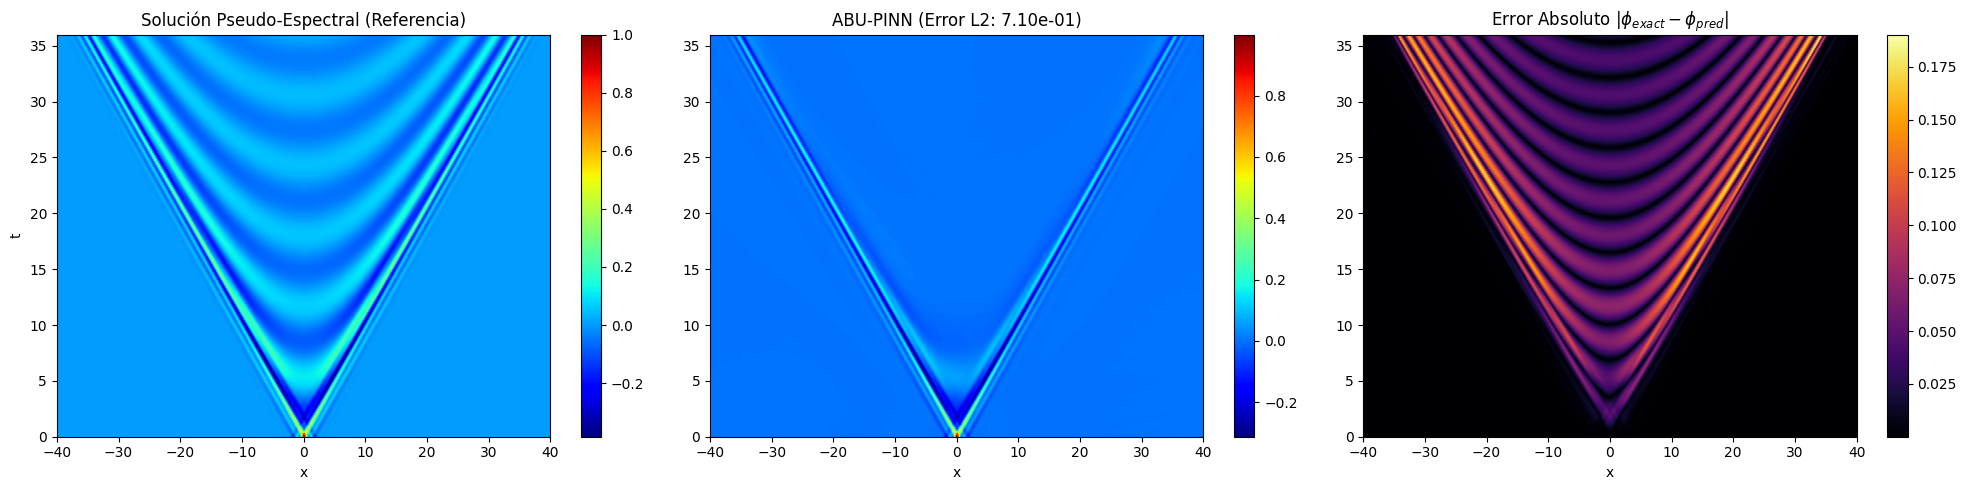
\includegraphics[width=\linewidth]{vanilla_error.png}\\[2mm]
  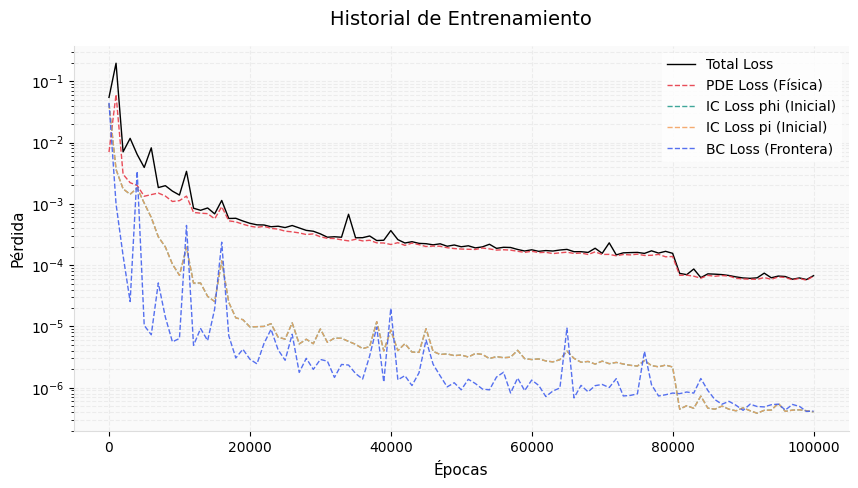
\includegraphics[width=0.55\linewidth]{vanilla_loss.png}
  \caption[Vanilla PINN: error map and training curves]{Vanilla PINN: L2RE 71.0\%. Large errors distributed over the whole region; the total loss oscillates and converges slowly, to values of order $10^{-5}$.}
  \label{fig:app-vanilla}
\end{figure}

\begin{figure}[htbp]
  \centering
  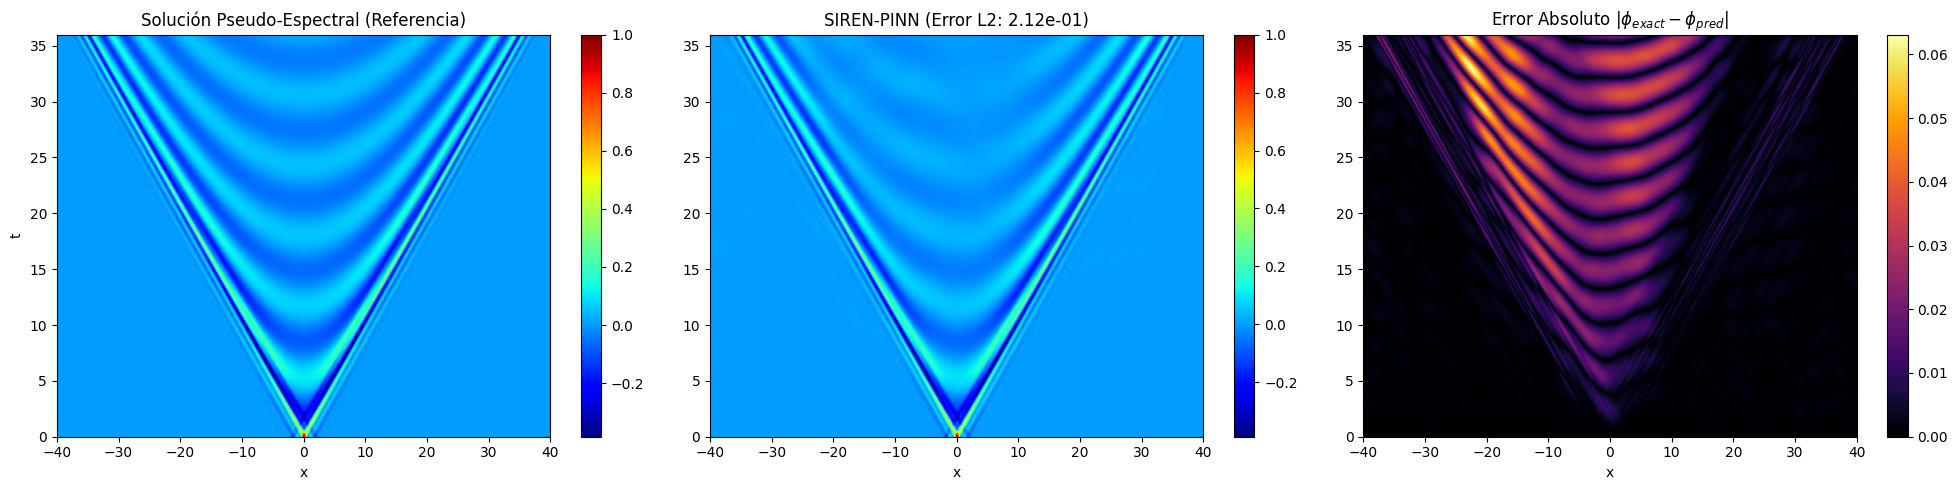
\includegraphics[width=\linewidth]{siren_error.png}\\[2mm]
  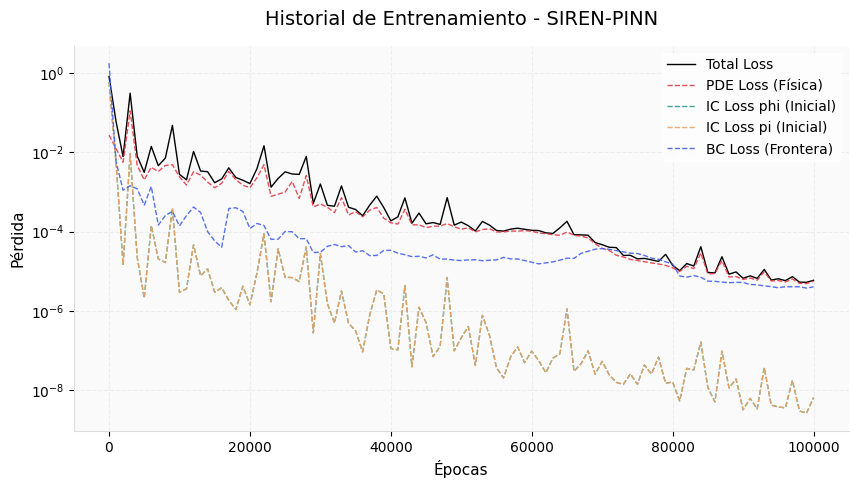
\includegraphics[width=0.55\linewidth]{siren_loss.png}
  \caption[PINN-SIREN: error map and training curves]{PINN-SIREN: L2RE 21.2\%. The maximum errors are reduced with respect to the vanilla PINN, with a better capture of the oscillations; the initial position loss reaches values close to $10^{-8}$.}
  \label{fig:app-siren}
\end{figure}

\begin{figure}[htbp]
  \centering
  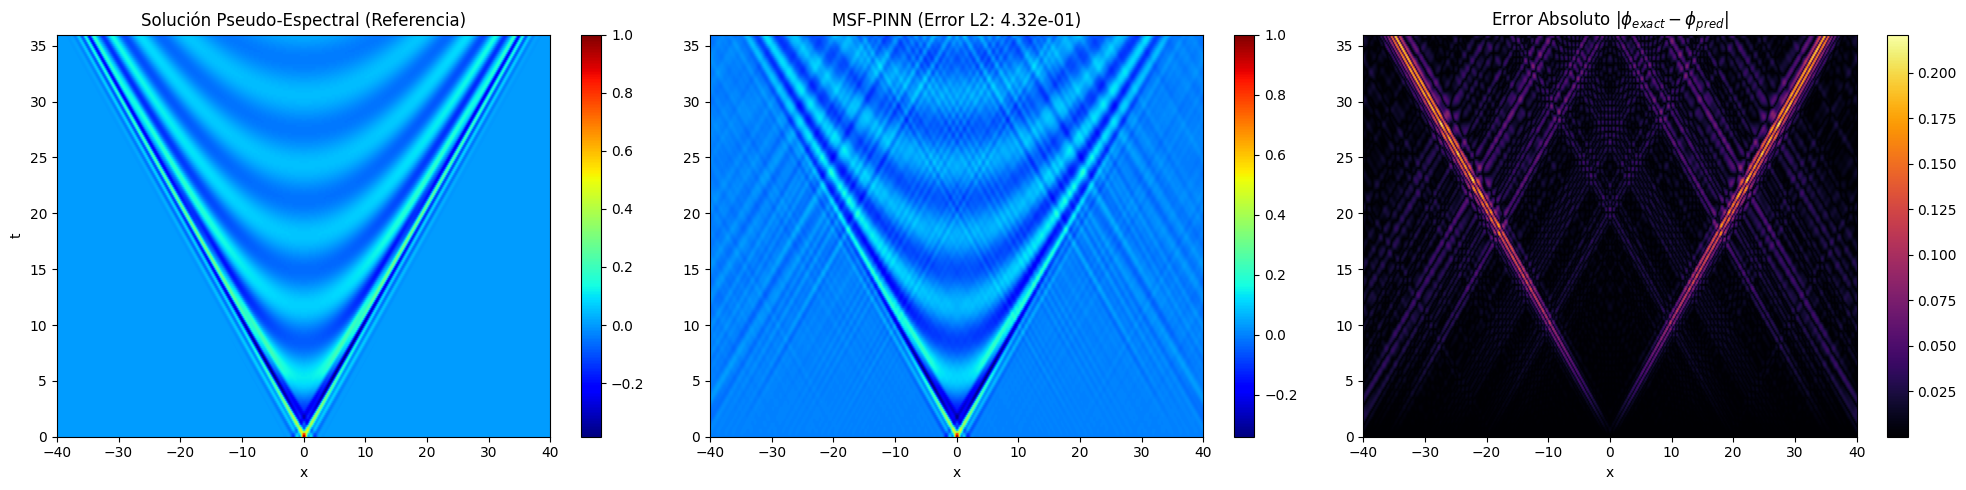
\includegraphics[width=\linewidth]{msf_error.png}\\[2mm]
  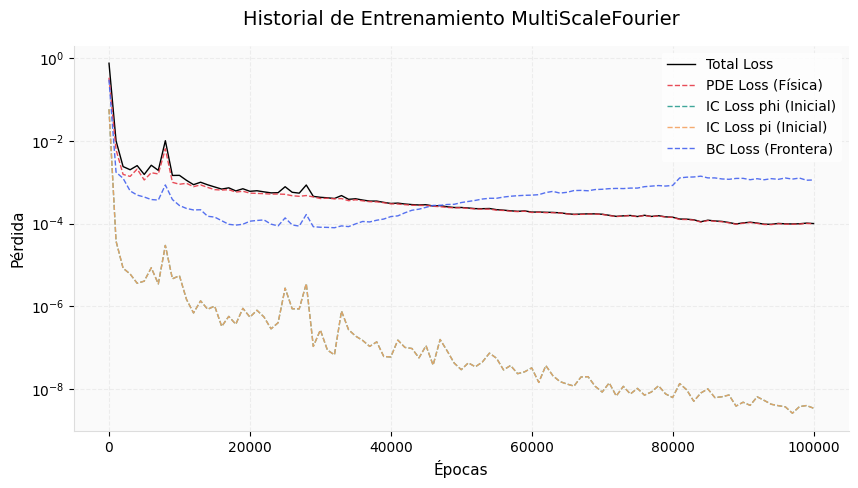
\includegraphics[width=0.55\linewidth]{msf_loss.png}
  \caption[MSF-PINN: error map and training curves]{MSF-PINN: L2RE 43.2\%. Despite the high number of parameters, the errors are significant, especially where the solution has high frequencies; the loss curves show high variance and poor convergence (order $10^{-4}$).}
  \label{fig:app-msf}
\end{figure}

\begin{figure}[htbp]
  \centering
  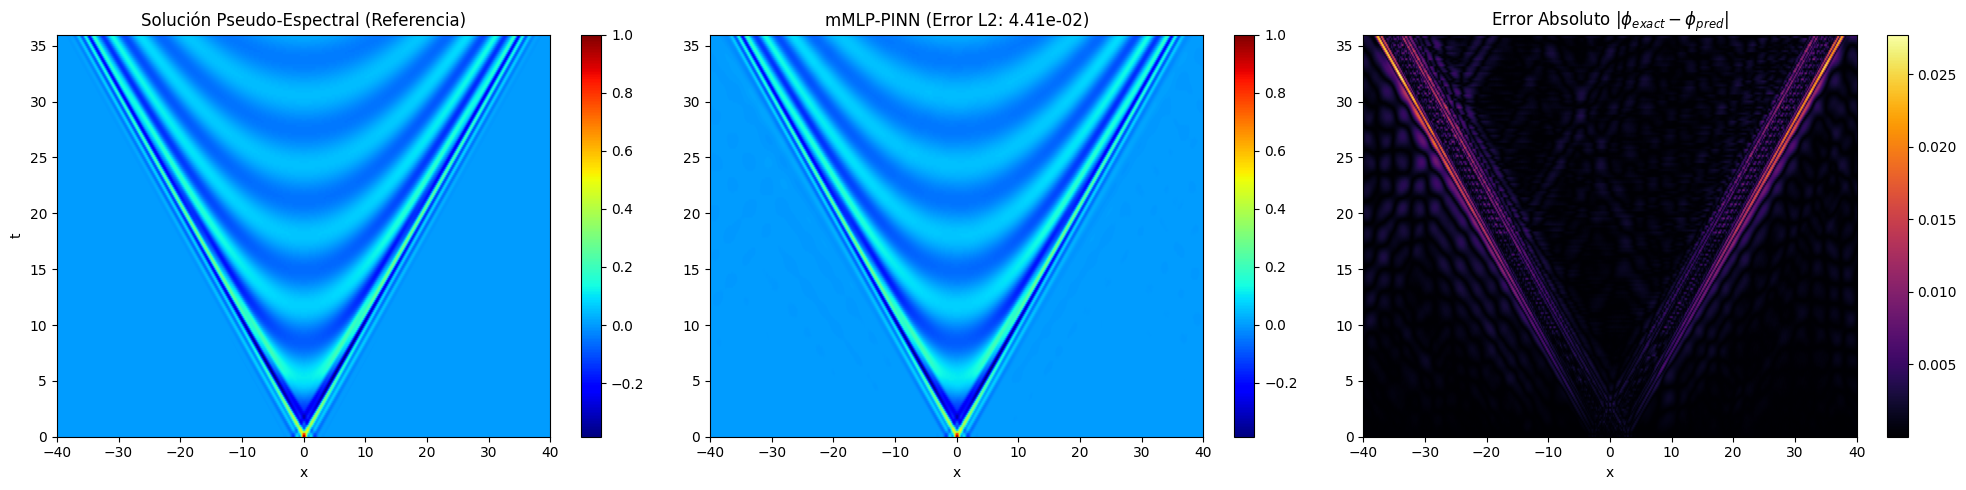
\includegraphics[width=\linewidth]{m4_error.png}\\[2mm]
  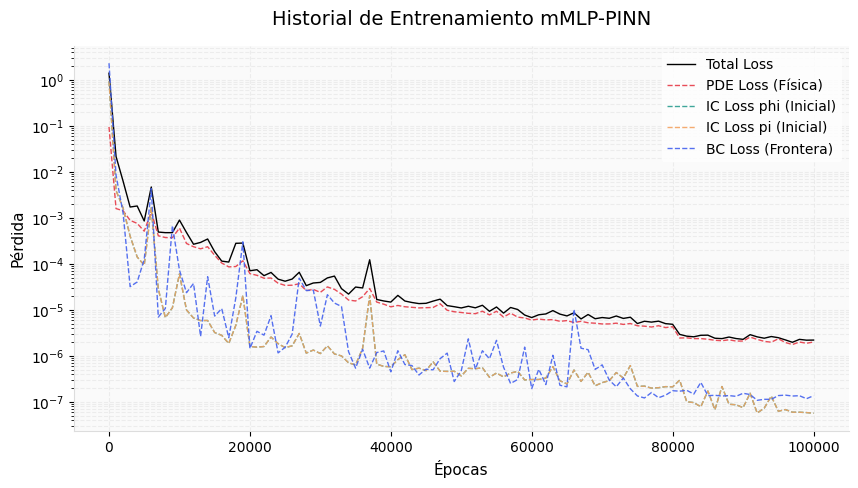
\includegraphics[width=0.55\linewidth]{m4_loss.png}
  \caption[M4-PINN: error map and training curves]{M4-PINN: L2RE 4.41\%. The maximum errors are drastically reduced, with a more homogeneous distribution; the total loss decreases rapidly and stabilizes at about $2.21\times10^{-6}$.}
  \label{fig:app-m4}
\end{figure}

\begin{figure}[htbp]
  \centering
  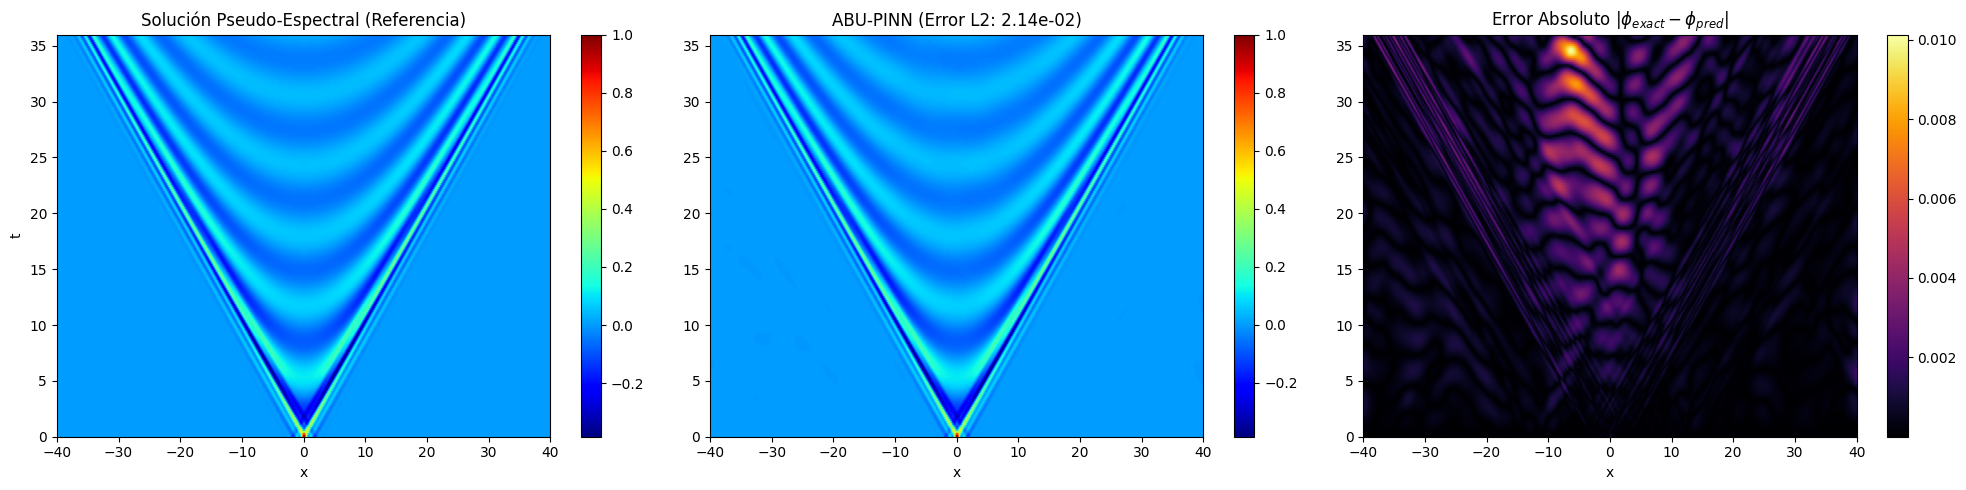
\includegraphics[width=\linewidth]{abu_error.png}\\[2mm]
  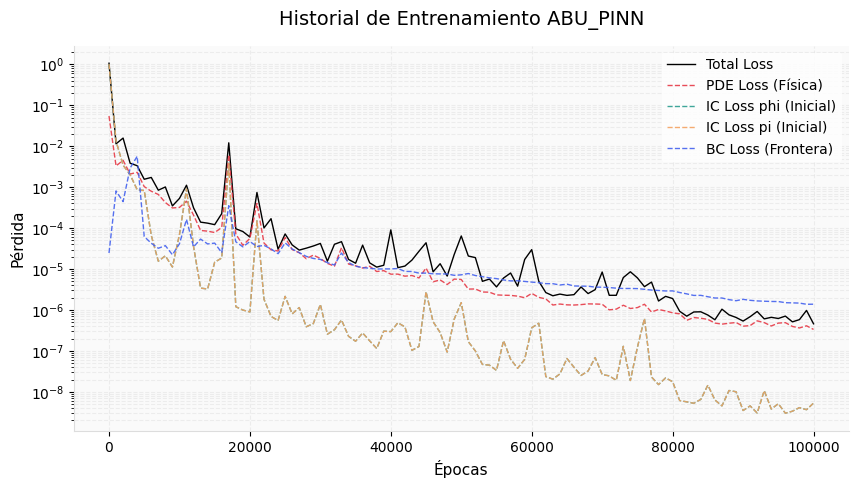
\includegraphics[width=0.55\linewidth]{abu_loss.png}
  \caption[AbuPINN: error map and training curves]{AbuPINN: L2RE 2.14\%. Homogeneous error without pronounced peaks; the total loss reaches $4.60\times10^{-7}$ with an almost stable and fast convergence.}
  \label{fig:app-abu}
\end{figure}

\begin{figure}[htbp]
  \centering
  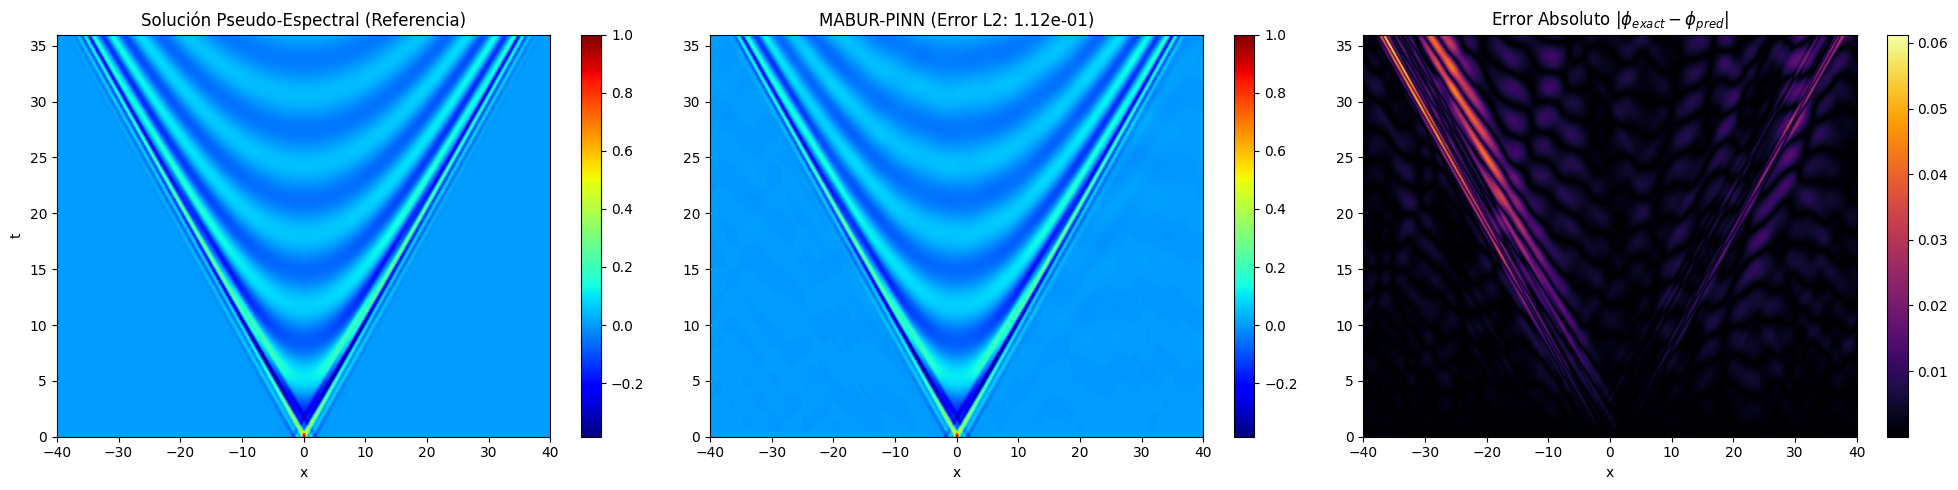
\includegraphics[width=\linewidth]{maburv1_error.png}\\[2mm]
  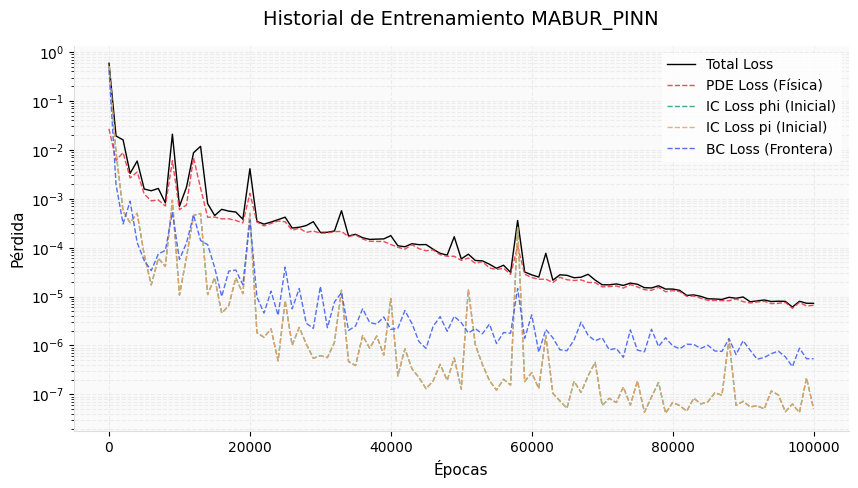
\includegraphics[width=0.55\linewidth]{maburv1_loss.png}
  \caption[MABUR-PINN V1: error map and training curves]{MABUR-PINN V1: L2RE 11.2\%. Improvements in the high-frequency regions with respect to MSF-PINN, but difficulties representing the frequencies inside the light cone; the total loss converges to about $7.25\times10^{-6}$.}
  \label{fig:app-maburv1}
\end{figure}

\begin{figure}[htbp]
  \centering
  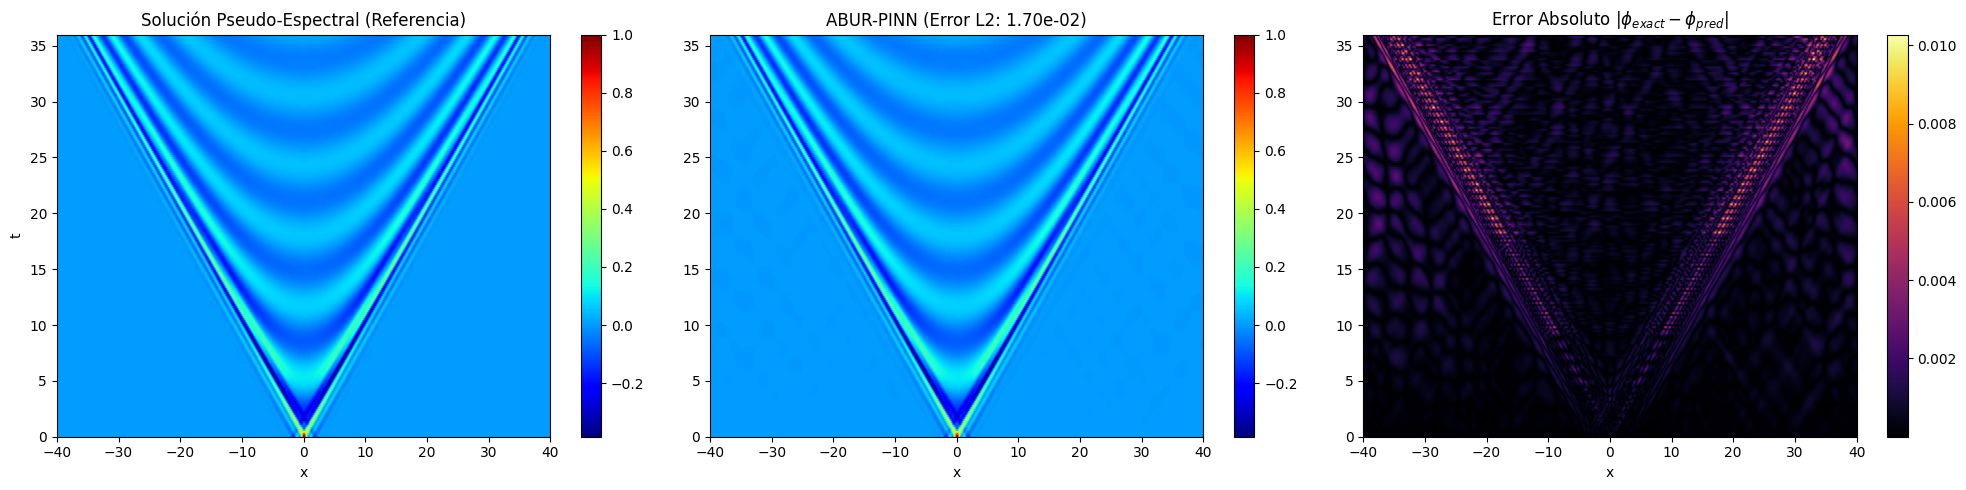
\includegraphics[width=\linewidth]{maburv2_error.png}\\[2mm]
  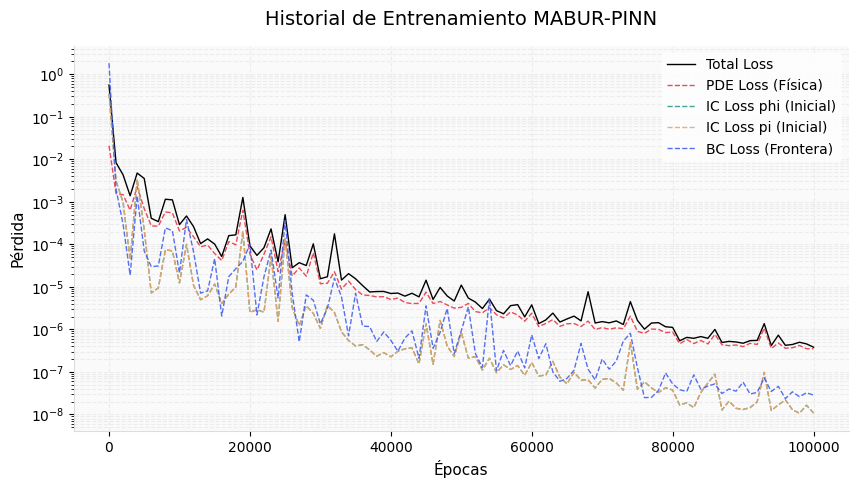
\includegraphics[width=0.55\linewidth]{maburv2_loss.png}
  \caption[MABUR-PINN V2: error map and training curves]{MABUR-PINN V2: L2RE 1.70\%. The error is concentrated on the fronts of the light cone; the total loss converges to $3.81\times10^{-7}$.}
  \label{fig:app-maburv2}
\end{figure}

\begin{figure}[htbp]
  \centering
  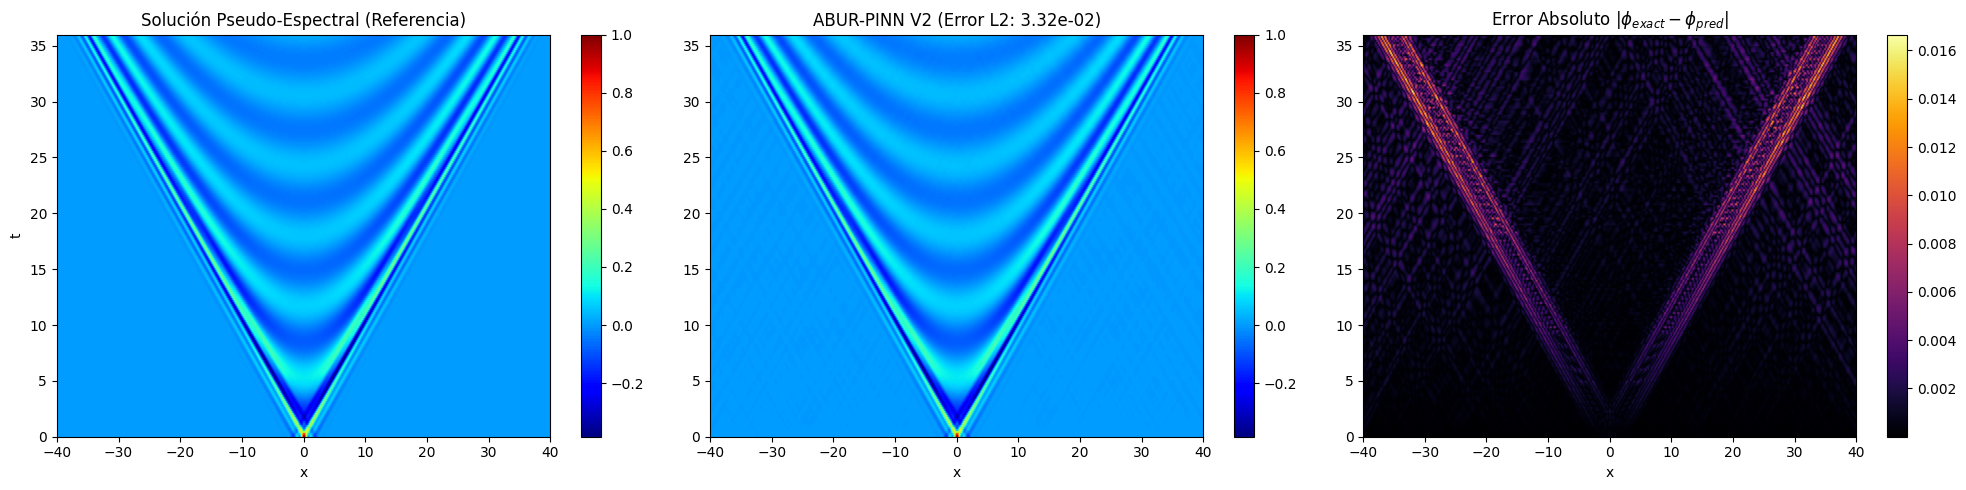
\includegraphics[width=\linewidth]{maburv2_sigma5_error.png}\\[2mm]
  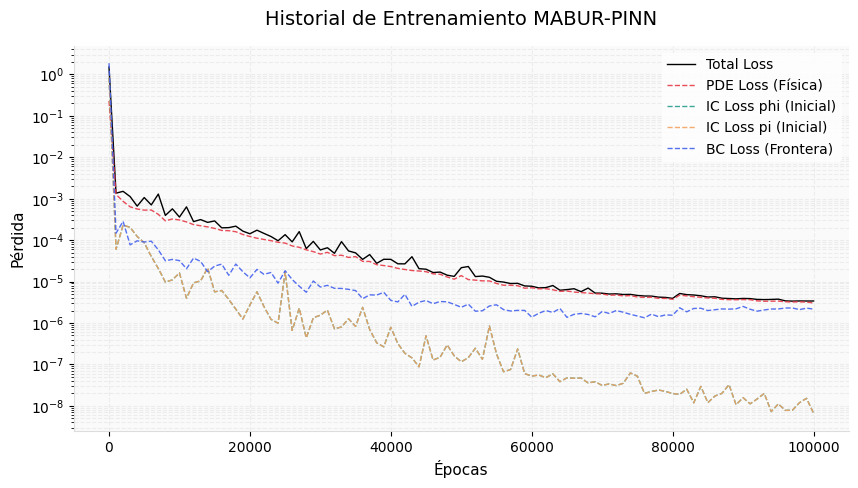
\includegraphics[width=0.55\linewidth]{maburv2_sigma5_loss.png}
  \caption{MABUR-PINN V2 ($\sigma=5$): L2RE 3.32\%. Same architecture with a larger Fourier scale.}
  \label{fig:app-maburv2_sigma5}
\end{figure}

\end{hyphenrules}
% Error Maps and Training Curves of Experiment 1
% !TEX root = 0000.tex
% Anexo F
% Contenido tomado de main_2.tex (líneas 4041-4048) sin cambios de texto.

% El texto está en inglés: reglas de corte de palabra del inglés
\begin{hyphenrules}{english}

\chapter{Anexo: Código y repositorio}\chaptermark{Código y repositorio}
All the code and results of this thesis are available in the following repositories:
\begin{itemize}
  \item Architectures and Klein--Gordon experiments (Chapter~\ref{ch:experiments}):
    \url{https://github.com/Emmaquantum/HPINN}
  \item Optimization study and pseudo-spectral reference solution:
    \url{https://github.com/Emmaquantum/Optimization_PINN}
\end{itemize}

\end{hyphenrules}
% Código y repositorio
\end{appendix}

%Permite visualizar la bibliografía en la tabla de contenido
%Cambie el nombre a Bibliografía o Literatura Citada en la siguiente línea de ser preciso
\addcontentsline{toc}{chapter}{Referencias Bibliográficas} 

\let\OLDthebibliography=\thebibliography
\def\thebibliography#1{\OLDthebibliography{#1}}
{\scriptsize
\pagestyle{plain}
% Nombre del documento donde se almacenan las referencias
\bibliography{Referencias}
% TESIS: \nocite{*} desactivado para que solo aparezcan las referencias citadas en el texto.
%\nocite{*}
% Inserta un página adicional al final en blanco 
%\cleardoublepage
% Para NO insertar una página adicional al final usar \clearpage
\clearpage
}}

\end{document}
